\chapter{Analisi Sintattica}\label{chap:syntactical}
%
\vspace*{-2ex}
\begin{center}
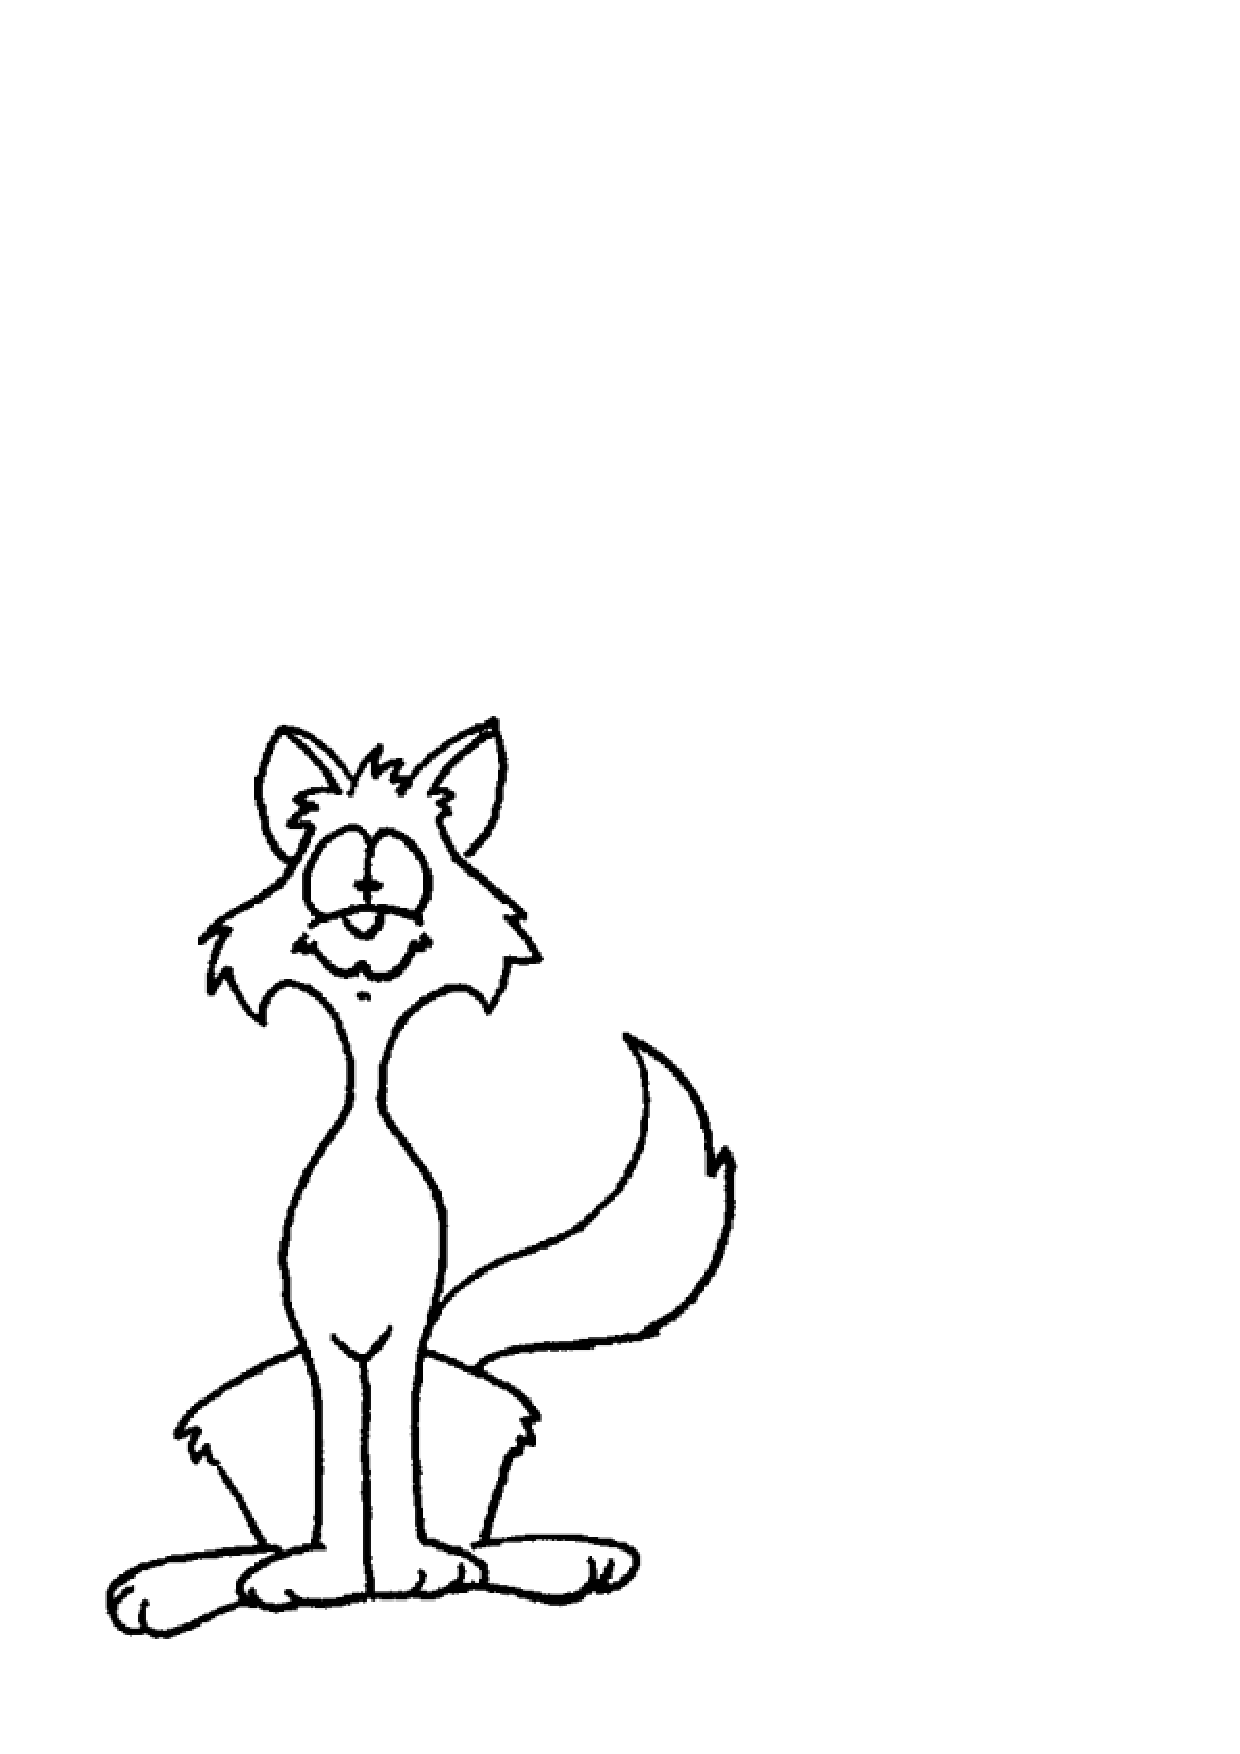
\epsfig{file = cat2.pdf, width = 3.5cm}
\end{center}
\vspace*{-2ex}
%
Abbiamo visto nel Capitolo~\ref{chap:lexical} come la sequenza di
caratteri di un sorgente Kitten viene trasformata in una lista
di \emph{token}. Programmi \emph{lessicalmente errati}, \cioe
contenenti sequenze di caratteri che non compongono alcun
token, vengono rifiutati dall'analizzatore lessicale con una segnalazione
di errore.

Non bisogna per\`o pensare che l'analizzatore lessicale impedisca
al programmatore di scrivere programmi \emph{sintatticamente errati}.
Per esempio, il comando \texttt{while (a != b a := a + 1} viene
tradotto nella sequenza di token \texttt{WHILE}, \texttt{LPAREN},
\texttt{ID}, \texttt{NEQ}, \texttt{ID}, \texttt{ID}, \texttt{ASSIGN},
\texttt{ID}, \texttt{PLUS}, \texttt{INTEGER} senza che alcun messaggio
di errore venga segnalato dall'analizzatore lessicale. Ci\`o nonostante,
tale comando \`e sintatticamente errato in quanto contiene una parentesi
tonda aperta che non \`e stata richiusa. In questo capitolo intendiamo
presentare delle tecniche che permettono di segnalare al programmatore
errori sintattici come quello appena mostrato. Tali tecniche sono
chiamate tecniche di analisi sintattica o di \emph{parsing}.
L'analisi sintattica ha due scopi:
%
\begin{itemize}
\item garantire
  che il codice rispetti le regole sintattiche del linguaggio. Se \cosi non
  \`e, un errore di sintassi deve essere segnalato al programmatore;
\item costruire una rappresentazione
  \emph{strutturata} del programma, detta \emph{sintassi astratta} del
  programma, che pu\`o essere \emph{comodamente}
  usata dalle successive fasi di analisi semantica e di generazione e
  ottimizzazione del codice.
\end{itemize}
%
\begin{figure}[t]
\begin{center}
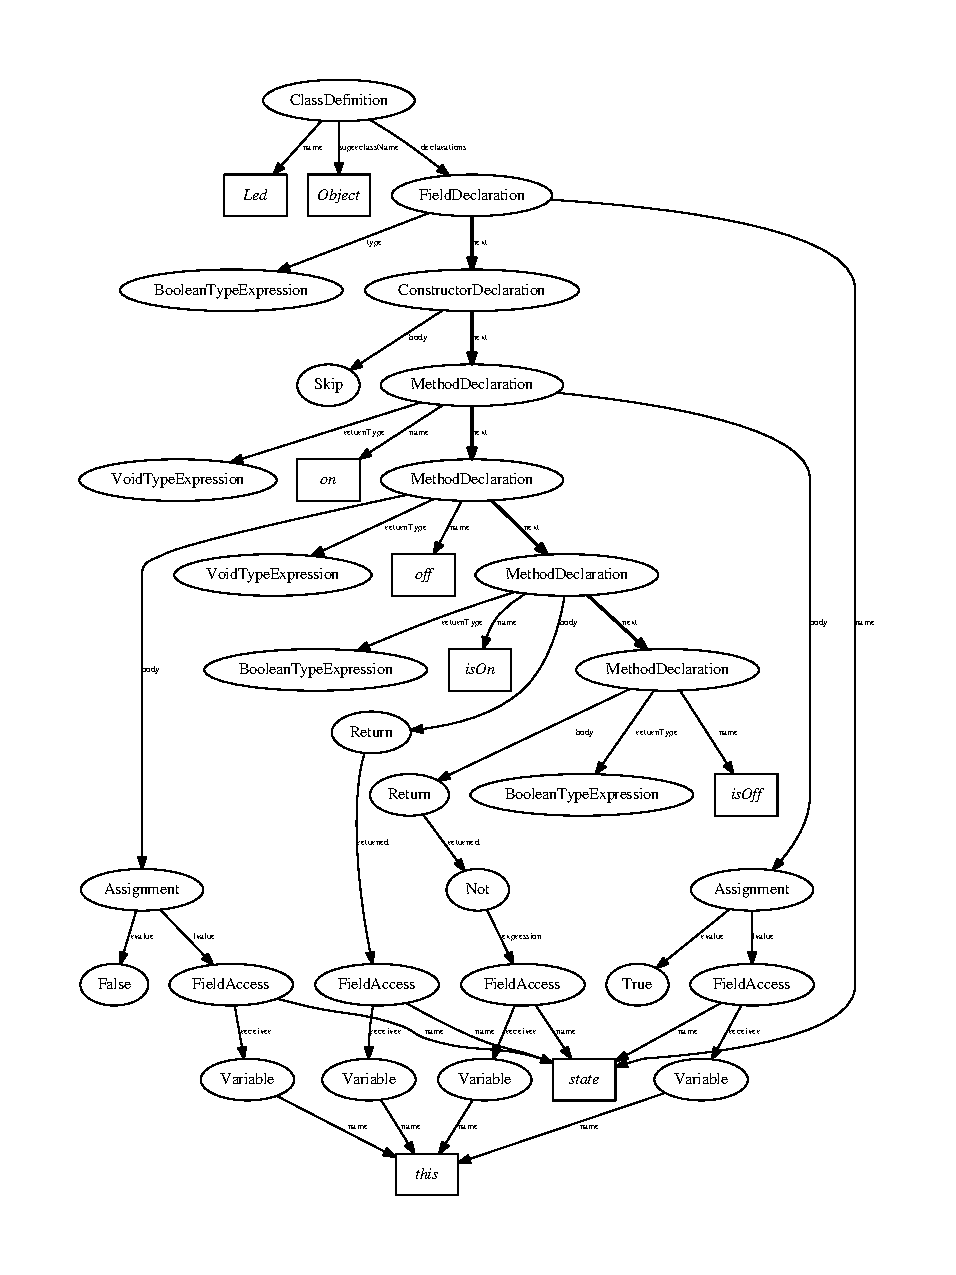
\epsfig{file = led_logica.pdf, height = 12.5cm}
\end{center}
\caption{La sintassi astratta del programma in Figura~\ref{fig:led}.}
  \label{fig:led_albero}
\end{figure}
%
Si consideri per esempio il programma in Figura~\ref{fig:led}. L'analisi
sintattica di Kitten accetta tale programma come sintatticamente corretto
e genera la sua struttura logica mostrata in Figura~\ref{fig:led_albero}.
Tale struttura logica \`e chiamata \emph{albero di sintassi astratta}
del programma la cui \emph{sintassi concreta} \`e in Figura~\ref{fig:led}.
Vedremo in futuro (Sezione~\ref{sec:abstract_syntax_classes})
come interpretare i nodi di questo albero. Per adesso
osserviamo solo che i nodi ovali rappresentano categorie di sintassi
astratta composte a partire dai sottoalberi ivi radicati. I nodi rettangolari
sono invece gli identificatori del programma e sono condivisi quando
occorrono pi\`u volte nel codice. In effetti, quindi, sarebbe pi\`u
corretto parlare di \emph{grafo} di sintassi astratta. Preferiamo comunque
continuare a chiamarlo albero dal momento che almeno
i nodi ovali sono raggiungibili tramite
un unico percorso a partire dalla radice dell'albero (posta in alto).
L'albero in Figura~\ref{fig:led_albero} \`e \piu \emph{comodo} da
maneggiare da parte di un computer che una sequenza di caratteri come
quella in Figura~\ref{fig:led}. Esso infatti \`e una vera e propria
struttura dati i cui diversi livelli di profondit\`a esprimono
la struttura del codice sorgente. Questa struttura \`e invece
meno evidente nel codice sorgente.

In questo capitolo parleremo, nell'ordine, delle \emph{grammatiche libere
dal contesto} (Sezione~\ref{sec:grammar}), che sono lo strumento che useremo
per descrivere la sintassi del codice sorgente di un programma.
Passeremo quindi a descrivere l'uso di uno strumento,
chiamato JavaCup, che permette di creare automaticamente
un analizzatore sintattico a partire dalla grammatica del linguaggio
che esso deve riconoscere (Sezione~\ref{sec:java_cup}).
Quindi analizzeremo il funzionamento di JavaCup, partendo
da un modo semplice ma poco potente di effettuare il parsing
(Sezione~\ref{sec:ll}) e passando quindi a una tecnica \piu
potente (Sezione~\ref{sec:lr}). Infine descriveremo la costruzione
dell'albero di sintassi astratta da parte di JavaCup
(Sezione~\ref{sec:abstract_syntax}) e la struttura dell'albero
di sintassi astratta stesso (Sezione~\ref{sec:abstract_syntax_classes}).
%
\section{Le grammatiche libere dal contesto}\label{sec:grammar}
%
La potenza delle espressioni regolari \`e limitata poich\'e esse
corrispondono a uno strumento di calcolo con una quantit\`a di memoria
limitata a priori (gli \emph{automi a stati finiti} della
Sezione~\ref{sec:nfa}). Esse non sono quindi in grado di esprimere
linguaggi la cui definizione richiede la capacit\`a di \emph{contare}
fino a livelli di profondit\`a arbitrari, come per esempio il linguaggio
%
\[
  P=\{\mathtt{a}^n\mathtt{b}^n\mid n\ge 0\}.
\]
Visto il primo carattere \texttt{b}, occorre ricordarsi quanti caratteri
\texttt{a} si sono visti per sapere quanti caratteri \texttt{b}
ci si deve ancora aspettare. Il \emph{linguaggio di parentesi} $P$ non \`e
un puro gioco teorico: esso astrae un tipico linguaggio di programmazione
la cui struttura \`e data da delimitatori come le parentesi graffe
o le parole chiave \texttt{begin} ed \texttt{end}.

Abbiamo visto nella Sezione~\ref{sec:modes} che le espressioni regolari
posso essere \emph{potenziate} utilizzando delle \emph{azioni con memoria}
(come l'assegnamento). Ma si tratta di una trucco scomodo per descrivere
la complessa sintassi di un linguaggio di programmazione. Meglio \`e invece
identificare uno strumento di descrizione di linguaggi strettamente \piu
potente delle espressioni regolari e naturalmente portato a descrivere la
sintassi dei linguaggi di programmazione. Questo strumento sono le
\emph{grammatiche libere dal contesto}.
%
\begin{definition}[Grammatica Libera dal Contesto]\label{def:grammar}
Una \emph{grammatica libera dal contesto} (in seguito semplicemente
\emph{grammatica}) su un alfabeto $\Lambda$
\`e una quadrupla $\langle T,N,I,P\rangle$ dove
\begin{itemize}
\item $T\subseteq\Lambda$
      \`e un insieme detto dei \emph{simboli terminali} o semplicemente
      dei \emph{terminali}
\item $N$ \`e un insieme
      detto dei \emph{simboli non terminali} o semplicemente
      dei \emph{non terminali}
\item $I\in N$ \`e il \emph{non terminale iniziale}
\item $P$ \`e un insieme di \emph{produzioni}, \cioe di frecce del tipo
      $L\to\gamma$ dove $L\in N$ \`e il \emph{lato sinistro} della produzione
      ed $\gamma\in (T\cup N)^*$ \`e una sequenza anche vuota di terminali e
      non terminali, detta \emph{lato destro} della produzione.
\end{itemize}
%
Indicheremo in grassetto i terminali, in italico
i non terminali e con lettere greche le sequenze, possibilmente vuote,
di terminali e non terminali, dette anche \emph{forme sentenziali}.
La forma sentenziale vuota sar\`a sempre indicata come $\varepsilon$. Si noti
che il lato destro di una produzione \`e una forma sentenziale.
Una forma sentenziale \`e detta \emph{ground} o \emph{stringa}
se non contiene non terminali.
\end{definition}

Un esempio di grammatica \`e la quadrupla $\langle T,N,I,P\rangle$ dove
%
\begin{equation}\label{eq:example_grammar}
\begin{split}
  T &= \{\mathtt{a},\mathtt{b}\}\\
  N &= \{I\}\\
  P &= \{I\to\varepsilon,\ I\to\mathtt{a}I\mathtt{b}\}.
\end{split}
\end{equation}
%
Essa \`e una grammatica per qualsiasi linguaggio che contenga almeno i simboli
$\mathtt{a}$ e $\mathtt{b}$. In futuro descriveremo una grammatica
semplicemente enumerando le sue produzioni. Assumeremo implicitamente
che $T$ \`e l'insieme dei terminali che occorrono nelle produzioni enumerate
e che $N$ \`e l'insieme dei non terminali che occorrono nelle produzioni
enumerate. Assumeremo inoltre che $I$ sia il non terminale a sinistra della
prima produzione.
%
\begin{definition}[Derivazione]\label{def:derivation}
Data una grammatica $G=\langle T,N,I,P\rangle$ e due forme sentenziali
$\alpha$ e $\beta$, diciamo che $\beta$ \`e
\emph{derivabile in $G$ in un passo}
da $\alpha$ se e solo se esiste una produzione
$L\to\gamma\in P$ tale che $\alpha=\eta L\delta$ e $\beta=\eta\gamma\delta$.
In tal caso scriveremo che $\alpha\Rightarrow_G\beta$.
Una \emph{derivazione} per $G$ \`e la concatenazione di pi\`u passi
di derivazione $\alpha\Rightarrow\beta_1\Rightarrow\beta_2\ldots$
Indicheremo con
$\Rightarrow^*_G$ la chiusura riflessiva e transitiva di $\Rightarrow$.
Quando $G$ \`e chiara dal contesto, eviteremo di indicarla esplicitamente
nelle notazioni $\Rightarrow$ e $\Rightarrow^*$.
\end{definition}
%
\noindent
Per esempio, nella grammatica~\eqref{eq:example_grammar} si ha
%
\begin{align*}
  \mathtt{ab}I\mathtt{b}&\Rightarrow\mathtt{aba}I\mathtt{bb}\\
  \mathtt{aba}I\mathtt{bb}&\Rightarrow\mathtt{ababb}\\
  I&\Rightarrow\mathtt{a}I\mathtt{b}\\
  I&\Rightarrow^*I\\
  \mathtt{ab}I\mathtt{b}&\Rightarrow^*\mathtt{ababb}.
\end{align*}

Le grammatiche servono a descrivere linguaggi, esattamente come gli automi a
stati finiti. In particolare, una grammatica genera il linguaggio formato
dalle stringhe derivabili dal non terminale iniziale.
%
\begin{definition}[Linguaggio generato da una grammatica]
  \label{def:gen_grammar}
Data una grammatica $G$ su un alfabeto $\Lambda$,
il linguaggio $L(G)$ da essa generato \`e
\[
  L(G)=\{\alpha\text{ ground}\mid I\Rightarrow^*\alpha\}.
\]
\end{definition}
%
\noindent
Per esempio, il linguaggio generato dalla grammatica~\eqref{eq:example_grammar}
\`e
%
\[
  L(G)=\{\mathtt{a}^n\mathtt{b}^n\mid n\ge 0\}=P.
\]
%
Questo mostra che le grammatiche libere dal contesto permettono di generare
linguaggi, come $P$, che non possono essere generati con automi a stati finiti.
Pi\`u in generale, si pu\`o
mostrare che ogni linguaggio generabile da un automa a stati
finiti \`e anche generabile da una grammatica libera dal contesto.
Conseguentemente, le grammatiche descrivono strettamente
pi\`u linguaggi che gli automi a stati finiti.

Data una forma sentenziale $\alpha$, potrebbe esserci pi\`u di un
$\beta$ tale che $\alpha\Rightarrow\beta$. Per esempio, nella
grammatica~\eqref{eq:example_grammar} abbiamo
$I\mathtt{b}\Rightarrow\mathtt{b}$
ma anche $I\mathtt{b}\Rightarrow\mathtt{a}I\mathtt{bb}$.
In questo caso abbiamo la possibilit\`a di scegliere quale produzione
usare per sostituire lo stesso non terminale $I$. In altri casi la
pluralit\`a delle scelte \`e la conseguenza di pi\`u occorrenze
di non terminali in $\alpha$. Si consideri per esempio la grammatica
%
\begin{equation}\label{eq:other_grammar}
\begin{split}
  I&\to\varepsilon\\
  I&\to\mathtt{a}\\
  I&\to\mathtt{b}\\
  I&\to II
\end{split}
\end{equation}
%
(come detto sopra, l'enumerazione delle produzioni \`e sufficiente
a definire la grammatica). La stessa stringa
$\mathtt{abb}$ possiamo derivarla tramite le derivazioni:
%
\begin{figure}[t]
\[
\xymatrix{
  & I\ar[ld]\ar[d]\ar[rd] \\
\mathtt{a} & I\ar[ld]\ar[d]\ar[rd] & \mathtt{b}\\
\mathtt{a} & I\ar[d] & \mathtt{b}\\
  & \varepsilon
}
\]
\caption{Un albero di derivazione per la
         grammatica~\eqref{eq:example_grammar}.}\label{fig:parse_tree}
\end{figure}
%
\begin{equation}\label{eq:many_derivations}
\begin{split}
  I&\Rightarrow II\Rightarrow I\mathtt{b}\Rightarrow II\mathtt{b}
    \Rightarrow\mathtt{a}I\mathtt{b}\Rightarrow\mathtt{abb}\\
  I&\Rightarrow II\Rightarrow III\Rightarrow II\mathtt{b}
    \Rightarrow\mathtt{a}I\mathtt{b}\Rightarrow\mathtt{abb}\\
  I&\Rightarrow II\Rightarrow I\mathtt{b}\Rightarrow II\mathtt{b}
    \Rightarrow I\mathtt{bb}\Rightarrow\mathtt{abb}.
\end{split}
\end{equation}
%
In questo caso la scelta riguarda l'ordine col quale sostituiamo le $I$.
Va osservato che questo secondo tipo di \emph{libert\`a di scelta} \`e
in effetti irrilevante, nel senso che, qualsiasi scelta si faccia, \`e poi
possibile effettuare un'altra sostituzione, temporaneamente
ritardata. Questa caratteristica delle grammatiche libere dal contesto dice
essenzialmente che il criterio con cui si sostituiscono i non terminali
in una forma sentenziale non cambia l'insieme delle stringhe
derivabili. Potremmo per esempio scegliere indifferentemente
di sostituire sempre prima
i non terminali pi\`u a sinistra (derivazioni \emph{leftmost}) o prima
quelli pi\`u a destra (derivazioni \emph{rightmost}).

Un modo per astrarre dall'ordine delle sostituzioni \`e quello di usare
degli \emph{alberi di parsing} al posto delle derivazioni stesse. Un albero
di parsing rappresenta un \emph{insieme} di derivazioni, tutte quelle
che derivano la stessa stringa, a partire dal non terminale
di partenza, con qualsiasi criterio di sostituzione.
%
\begin{definition}[Albero di parsing o di derivazione]\label{def:parsing_tree}
Un \emph{albero di parsing} o \emph{di derivazione}
per una grammatica $G=\langle T,N,I,P\rangle$ \`e un albero tale che:
\begin{enumerate}
\item i suoi nodi sono etichettati con un elemento di $N$ o di $T$ o con
      $\varepsilon$;
\item la radice \`e etichettata con $I$
\item le foglie sono etichettate con elementi di $T$ o con $\varepsilon$
\item dato un nodo etichettato come $L$ e prese, da sinistra a destra,
      le etichette $e_1,\ldots,e_n$ dei suoi figli, allora
      $L\to e_1\cdots e_n\in P$.
\end{enumerate}
La concatenazione delle etichette della
frontiera dell'albero, letta da sinistra a destra secondo una visita
leftmost in profondit\`a, \`e la stringa
\emph{derivata} dall'albero a partire dalla sua radice.
\end{definition}
%
\noindent
Per esempio, la Figura~\ref{fig:parse_tree} mostra un albero di derivazione
per la grammatica~\eqref{eq:example_grammar}. Esso deriva la stringa
$\mathtt{aabb}$ e astrae l'insieme di derivazioni
\[
  \{I\Rightarrow\mathtt{a}I\mathtt{b}\Rightarrow\mathtt{aa}I\mathtt{bb}
    \Rightarrow\mathtt{aabb}\}.
\]
%
L'albero a sinistra nella Figura~\ref{fig:ambiguity} \`e un albero di
derivazione per la grammatica~\eqref{eq:other_grammar}. Esso deriva la stringa
$\mathtt{abb}$ e astrae un insieme di derivazioni che include, fra
le altre, le derivazioni~\eqref{eq:many_derivations}.

Gli alberi di derivazione rappresentano insiemi di derivazioni che possiamo
considerare equivalenti e interscambiabili. In particolare,
un albero di derivazione
specifica la struttura logica delle derivazioni che esso rappresenta:
come cio\`e la stringa sulla sua frontiera viene costruita
a partire dal non terminale iniziale, senza entrare nei dettagli dell'ordine
con cui questa costruzione \`e effettuata. Ne consegue che, se una stessa
stringa $\alpha$ ammette due alberi di derivazione diversi, allora
ci sono almeno due modi, \emph{strutturalmente diversi}, di derivare $\alpha$.
%
\begin{figure}[t]
\[
\xymatrix{
   &   & I\ar[ld]\ar[rd] \\
   & I\ar[ld]\ar[rd] &   & I\ar[d]\\
 I\ar[d] &   & I\ar[d] & \mathtt{b}\\
 \mathtt{a} & & \mathtt{b}
}
\qquad\qquad\qquad
\xymatrix{
  & I\ar[ld]\ar[rd] \\
I\ar[d] &   & I\ar[ld]\ar[rd]\\
\mathtt{a} & I\ar[d] &  & I\ar[d]\\
  & \mathtt{b} &  & \mathtt{b}
}
\]
\caption{Due alberi di derivazione diversi per la stessa stringa $\mathtt{abb}$.}\label{fig:ambiguity}
\end{figure}
%
\begin{definition}[Grammatica ambigua]\label{def:ambiguity}
Una grammatica $G$ \`e \emph{ambigua} se e solo se esiste una forma
sentenziale ground $\alpha$ che ammette due alberi di parsing diversi in $G$.
\end{definition}
%
\noindent
Per esempio, la grammatica~\eqref{eq:other_grammar} \`e ambigua poich\'e
ammette due alberi di derivazione diversi per la stringa
$\mathtt{abb}$, come mostrato in Figura~\ref{fig:ambiguity}.

Le grammatiche ambigue ci porranno dei problemi poich\'e non specificano
un'unica struttura per le stringhe di un linguaggio, ma danno la
possibilit\`a di interpretarle strutturalmente in modo diverso. Per esempio,
la Figura~\ref{fig:ambiguity} mostra che la stringa $\mathtt{abb}$ pu\`o
essere interpretata nella grammatica~\eqref{eq:other_grammar}
come la stringa $\mathtt{ab}$ seguita da una
$\mathtt{b}$ (albero a sinistra)
o come una $\mathtt{a}$ seguita dalla stringa $\mathtt{bb}$ (albero a destra). 
\`E quindi importante riuscire a scrivere grammatiche non ambigue, sebbene
non esistano vere e proprie regole per farlo. Per esempio, il linguaggio
della grammatica ambigua~\eqref{eq:other_grammar}
\`e l'insieme di tutte le stringhe di
$\mathtt{a}$ e di $\mathtt{b}$. Questa semplice osservazione ci
convince che possiamo generare lo stesso linguaggio tramite
la grammatica non ambigua:
%
\begin{align*}
  I&\to\varepsilon\\
  I&\to\mathtt{a}I\\
  I&\to\mathtt{b}I.
\end{align*}
%
\begin{exercise}\label{ex:lists}
Si definisca una grammatica sull'alfabeto $\{\mathtt{a},\mathtt{b}\}$ che
genera tutte e sole le sequenze (o liste) non vuote di $\mathtt{a}$.
Si definisca quindi un'altra grammatica che genera tutte e sole le sequenze,
possibilmente vuote, di $\mathtt{a}$.
\end{exercise}
%
\begin{exercise}\label{ex:as_many_as}
Si definisca una grammatica sull'alfabeto $\{\mathtt{a},\mathtt{b}\}$ che
genera tutte e sole le sequenze di $\mathtt{a}$ e di $\mathtt{b}$ che
contengono tante $\mathtt{a}$ quante $\mathtt{b}$. La grammatica che
avete ottenuto \`e ambigua?
\end{exercise}
%
\section{La generazione dell'analizzatore sintattico di Kitten}
  \label{sec:java_cup}
%
Specificheremo la sintassi concreta di Kitten tramite una grammatica
libera dal contesto. Si noti che questo non ci permetter\`a
di specificare alcuni
aspetti sintattici del linguaggio che non sono specificabili tramite
grammatiche libere dal contesto. Per esempio, non saremo capaci di specificare
il fatto che un identificare deve essere dichiarato prima di poter
essere usato, \nec l'uso corretto dei tipi nelle espressioni. Questi aspetti
verranno quindi considerati \emph{semantici} e gestiti in seguito, in fase,
appunto, di analisi semantica (Capitolo~\ref{chap:semantical}).

La creazione di un parser a partire dalla grammatica di
Kitten verr\`a ottenuta in maniera automatica, tramite uno strumento Java
di nome JavaCup. Esso \`e una versione Java di un vecchio programma C
di nome \texttt{yacc}~\cite{Johnson75}.
Dal momento che vogliamo riconoscere il linguaggio Kitten, useremo
in JavaCup la grammatica per tale linguaggio.
La Figura~\ref{fig:java_cup} mostra l'utilizzo di JavaCup.
L'applicazione di JavaCup alla grammatica del linguaggio
Kitten, specificata dentro un file \texttt{syntactical/Kitten.cup},
produce tre file:
%
\begin{enumerate}
\item l'analizzatore sintattico vero e proprio
      \texttt{syntactical/Parser.java}. Esso pu\`o quindi
      essere compilato con \texttt{javac} ed eseguito per effettuare il parsing
      di un programma Kitten;
\item il file \texttt{syntactical/sym.java}, che enumera i terminali
      (token) usati dalla grammatica, associando loro un identificatore
      intero unico; si tratta dello stesso file usato dall'analizzatore
      lessicale per identificare i token (Sezione~\ref{sec:jlex});
\item il file di log \texttt{syntactical/Kitten.err}. Tale file contiene
      eventuali errori nella specifica della grammatica o eventuali
      problemi riscontrati da JavaCup, quando per esempio non riesce a
      creare il parser a causa di una grammatica non adeguata.
      Questo file contiene anche gli stati di un automa di cui parleremo
      in Sezione~\ref{sec:lr}.
\end{enumerate}
%
\javatip{Se qualcosa non funziona nella generazione del parser dalla
grammatica, il programma JavaCup non comunica messaggi di errore da linea
di comando ma scrive tutto nel file \texttt{syntactical/Kitten.err}.
Se quindi, dopo aver modificato o sostituito la grammatica Kitten, JavaCup
non genera l'analizzatore \texttt{syntactical/Parser.java}, si vada a guardare
il contenuto di \texttt{syntactical/Kitten.err}.}

Vedremo nelle Sezioni~\ref{sec:ll} e~\ref{sec:lr} due modi per
generare l'analizzatore sintattico a partire dalla specifica di una grammatica;
in particolare, quello descritto nella Sezione~\ref{sec:lr} \`e quello
utilizzato da JavaCup. Nella Sezione~\ref{sec:abstract_syntax} vedremo
come usare JavaCup per generare anche l'albero che descrive la struttura
del file sorgente, come quello mostrato in Figura~\ref{fig:led}.
Per adesso descriviamo la specifica della grammatica
Kitten contenuta nel file \texttt{syntactical/Kitten.cup}.
%
\begin{figure}[t]
\begin{center}
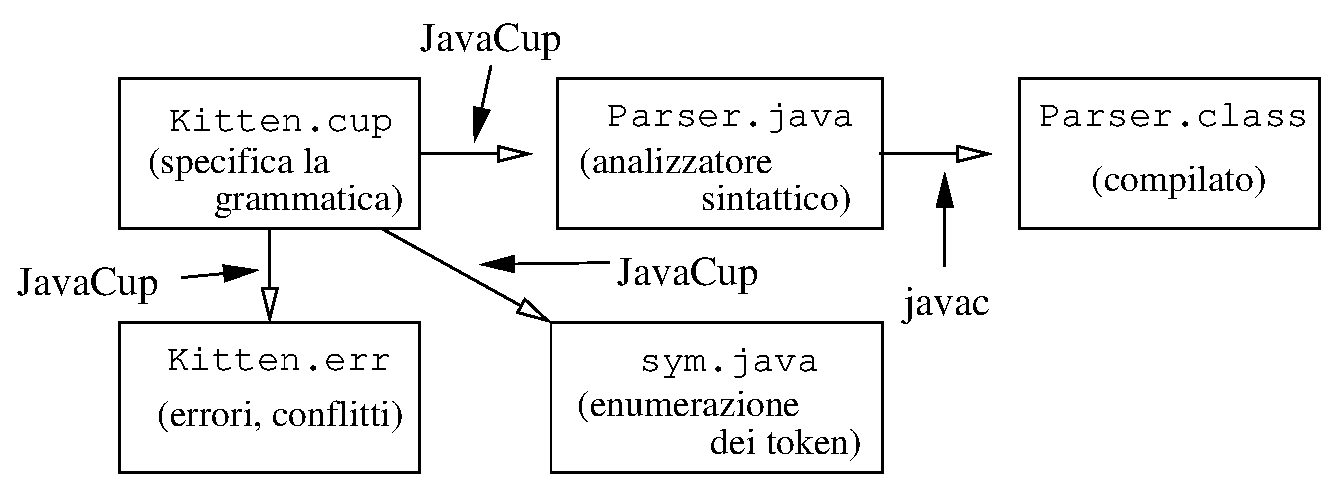
\epsfig{file = java_cup.eps, width = 11cm}
\end{center}
\caption{La generazione dell'analizzatore sintattico tramite JavaCup.}
  \label{fig:java_cup}
\end{figure}
%
\subsection{La specifica dei terminali e dei non terminali}
  \label{subsec:terminals}
%
Il file \texttt{syntactical/Kitten.cup}
inizia con l'enumerazione dei terminali della grammatica:
%
\begin{verbatim}
  terminal ID, STRING, INTEGER, FLOATING,
           CLASS, EXTENDS, FIELD, METHOD, CONSTRUCTOR, NEW,
           INT, FLOAT, BOOLEAN, VOID,
           COMMA, SEMICOLON, AS, LPAREN, RPAREN,
           LBRACK, RBRACK, LBRACE, RBRACE, DOT, PLUS, MINUS,
           TIMES, DIVIDE, EQ, NEQ, LT, LE, GT, GE, AND, OR, NOT,
           ASSIGN, ARRAY, IF, THEN, ELSE, WHILE, FOR,
           OF, RETURN, NIL, TRUE, FALSE, UMINUS;
\end{verbatim}
%
Si noti che essi, tranne \texttt{UMINUS} (Sezione~\ref{subsec:priorities}),
sono esattamente gli stesso terminali (token) generati
dall'analizzatore lessicale del Capitolo~\ref{chap:lexical}. L'ordine
con cui essi sono enumerati non ha normalmente importanza, ma
ritorneremo su questo aspetto.
Segue quindi una enumerazione dei non terminali\footnote{
Non scriviamo i non terminali
in italico poich\'e si tratta di un file testo che viene passato a JavaCup.}
della grammatica:
%
\begin{verbatim}
  non terminal class;
  non terminal class_members;
  non terminal formals;
  non terminal formals_aux;
  non terminal statements;
  non terminal command;
  non terminal exp;
  non terminal expseq;
  non terminal expseq_aux;
  non terminal lvalue;
  non terminal type;
  non terminal typeplus;
\end{verbatim}
%
Un ben preciso non terminale \`e marcato come non terminale iniziale della
grammatica:
%
\begin{verbatim}
  start with class;
\end{verbatim}
%
Questo significa che un programma Kitten deve essere derivabile a partire
dal non terminale \texttt{class} ovvero, per come daremo le produzioni di
\texttt{class}, che un programma Kitten non \`e altro che una definizione
di una classe, che eventualmente usa altre classi definite in altri file
sorgenti.

Seguono a questo punto le produzioni della grammatica per ogni non terminale
del linguaggio enumerato sopra. Li commenteremo secondo un ordine bottom-up,
partendo \cioe da tipi, espressioni e comandi e andando verso
il non terminale per la classe.
%
\subsection{La specifica dei tipi Kitten}\label{subsec:types_specification}
%
I tipi Kitten sono descritti dalle seguenti produzioni:
%
\begin{verbatim}
  type ::=
     ID
   | BOOLEAN
   | INT
   | FLOAT
   | ARRAY OF type ;
\end{verbatim}
%
La barra verticale indica un'alternativa nella definizione di \texttt{type}.
Si noti che oltre ai tre tipi primitivi \texttt{boolean}, \texttt{int}
e \texttt{float}, sono previsti dei tipi classe, espressi come il token
\texttt{ID}, nonch\'e il tipo array, definito ricorsivamente.
Il non terminale \texttt{type} \`e usato quando si vuole specificare
il tipo di una variabile, per esempio in una dichiarazione, o in una
espressione, come in un cast. Se vogliamo invece specificare il tipo
di ritorno di un metodo useremo il
non terminale \texttt{typeplus} che ammette anche il tipo \texttt{void}:
%
\begin{verbatim}
  typeplus ::=
     type
   | VOID ;
\end{verbatim}
%
\subsection{La specifica delle espressioni Kitten}
  \label{subsec:expressions_specification}
%
Un'espressione (Sezione~\ref{sec:expressions})
\`e definita in maniera ricorsiva tramite le seguenti produzioni:
%
\begin{verbatim}
  exp ::=
     lvalue                          // leftvalue
   | TRUE                            // la costante true
   | FALSE                           // la costante false
   | INTEGER                         // una costante intera
   | FLOATING                        // una costante in virgola mobile
   | STRING                          // una costante stringa fra apici
   | NIL                             // il riferimento costante nil
   | NEW ID LPAREN expseq RPAREN     // la creazione di un oggetto
   | NEW type LBRACK exp RBRACK      // la creazione di un array
   | exp AS type                     // un cast o conversione di tipo
   | exp PLUS exp                    // un'addizione
   | exp MINUS exp                   // una sottrazione
   | exp TIMES exp                   // una moltiplicazione
   | exp DIVIDE exp                  // una divisione
   | MINUS exp                       // l'opposto di un valore intero
   | exp LT exp                      // <
   | exp LE exp                      // <=
   | exp GT exp                      // >
   | exp GE exp                      // >=
   | exp EQ exp                      // uguaglianza
   | exp NEQ exp                     // disuguaglianza
   | exp AND exp                     // and logico
   | exp OR exp                      // or logico
   | NOT exp                         // negazione logica
   | exp DOT ID LPAREN expseq RPAREN // chiamata di metodo non void
   | LPAREN exp RPAREN ;             // parentesi
\end{verbatim}
%
Tali produzioni dicono in primo luogo che i \emph{leftvalue} sono
espressioni. In effetti, tutte le espressioni possono essere usate
alla destra di un assegnamento (come \emph{rightvalue}) ma
una categoria ristretta di espressioni, dette \emph{leftvalue}, pu\`o
essere usata \emph{anche} alla sinistra di un assegnamento.
A tal fine, tali espressioni devono fare riferimento a una ben precisa
cella di memoria dentro la quale l'assegnamento pu\`o scrivere.
Ci sono solo tre tipi di leftvalue in Kitten:
%
\begin{enumerate}
\item le variabili, come in \texttt{a := 35}; in questo caso l'assegnamento
      modifica la cella di memoria che contiene il valore della variabile
      \texttt{a};
\item i campi degli oggetti, come in \texttt{o.f := a}; in questo caso
      l'assegnamento modifica la cella di memoria che contiene il valore
      del campo \texttt{f} dell'oggetto contenuto nella variabile
      \texttt{o};
\item gli elementi degli array, come in \texttt{arr[i] := a}; in questo caso
      l'assegnamento modifica la cella $i$-esima dell'array \texttt{arr}.
\end{enumerate}
%
Conseguentemente, la specifica dei leftvalue \`e data tramite le seguenti
produzioni:
%
\begin{verbatim}
  lvalue ::=
     ID                              // una variabile
   | exp DOT ID                      // il campo di un oggetto
   | exp LBRACK exp RBRACK ;         // un elemento di un array
\end{verbatim}
%
Si noti che la sintassi di espressioni e leftvalue \`e mutuamente ricorsiva.

Le precedenti produzioni per \texttt{exp} dicono anche
che tutte le costanti del linguaggio sono espressioni:
\cioe \texttt{true}, \texttt{false}, le costanti intere, le costanti in virgola
mobile, le stringhe fra doppi apici e il riferimento \texttt{nil}.
\`E un'espressione anche la creazione di un oggetto come in
\texttt{new Rettangolo(10,20)}. Questo \`e ottenuto tramite la
produzione per \texttt{exp}:
%
\begin{verbatim}
  exp ::= NEW ID LPAREN expseq RPAREN
\end{verbatim}
%
dove \texttt{ID} \`e l'identificatore della classe che si sta istanziando
e \texttt{expseq} \`e una sequenza, possibilmente vuota, di espressioni
separate da virgole:
%
\begin{verbatim}
  expseq ::=
   | expseq_aux ;

  expseq_aux ::=
     exp
   | exp COMMA expseq_aux ;
\end{verbatim}
%
Si noti che la prima produzione per \texttt{expseq}
\`e una $\varepsilon$-produzione.

La creazione di un array specifica sia il tipo dei suoi elementi che la
dimensione dell'array, come in \texttt{new int[50]}, ed \`e ottenuta tramite
la produzione
%
\begin{verbatim}
  exp ::= NEW type LBRACK exp RBRACK
\end{verbatim}
%
Kitten non ammette la creazione diretta di array multidimensionali. Essi devono
quindi essere creati a partire da un array monodimensionale i cui elementi
sono a loro volta degli array che vanno essi stessi
creati esplicitamente come array monodimensionali.

Il cast viene effettuato in Kitten con la notazione \texttt{as}, come in
\texttt{persona as Studente}. Questa sintassi \`e resa possibile dalla
produzione:
%
\begin{verbatim}
  exp ::= exp AS type
\end{verbatim}
%
Si noti che \texttt{type} non \`e vincolato in alcun modo (tranne a non essere
\texttt{void}, infatti abbiamo usato \texttt{type} e non \texttt{typeplus}).
\`E quindi del tutto lecito scrivere \texttt{12 as float} oppure
\texttt{arr as array of int}. In particolare, la stessa notazione viene
usata sia per le conversioni di tipo (\texttt{12 as float}) che per
i cast veri e propri (\texttt{persona as Studente} e
\texttt{arr as array of int}).

Le precedenti produzioni per le espressioni includono le operazioni
binarie, sia aritmetiche (addizione, sottrazione, moltiplicazione e
divisione) che di confronto (maggiore, maggiore o uguale, minore, minore
o uguale, uguale, diverso) che logiche (and logico e or logico).
Infine includono le due operazioni unarie di negazione di interi
(\texttt{MINUS}) e di valori logici (\texttt{NOT}) e l'espressione
per la chiamata di metodo che non ritorna \texttt{void}
(Sezione~\ref{sec:expressions}), ottenuta con la produzione:
%
\begin{verbatim}
  exp ::= exp DOT ID LPAREN expseq RPAREN
\end{verbatim}
%
in cui, come si pu\`o vedere, \`e richiesta la presenza esplicita
del ricevitore della chiamata.

Infine, una espressione fra parentesi tonde viene ancora considerata
come un'espressione. Questo permette per esempio
di cambiare la precedenza degli operatori aritmetici rispetto a quella
di default, descritta nella prossima sezione.
%
\subsection{La specifica della precedenza degli operatori aritmetici}
  \label{subsec:priorities}
%
La grammatica per le espressioni aritmetiche della sezione precedente
\`e chiaramente ambigua. Per esempio, l'espressione
\texttt{2 + a * 4} pu\`o essere interpretata sia come
\texttt{(2 + a) * 4} che come \texttt{2 + (a * 4)}. Abbiamo gi\`a anticipato
che le grammatiche ambigue ci porranno problemi in fase di creazione
dell'analizzatore sintattico, il quale essenzialmente non sa quale delle
due interpretazioni preferire. Sappiamo dall'esperienza con altri linguaggi
di programmazione che la moltiplicazione ha \emph{precedenza} rispetto
all'addizione, per cui l'interpretazione da preferire \`e
\texttt{2 + (a * 4)}. Un problema simile sorge di fronte ad espressioni come
\texttt{2 - a - 4} che sono normalmente intese come
\texttt{(2 - a) - 4} piuttosto che come \texttt{2 - (a - 4)}. Si noti che
queste due interpretazioni sono diverse poich\'e, se \texttt{a} valesse
$0$, la prima interpretazione darebbe a
\texttt{2 - a - 4} il valore $-2$ mentre la seconda le darebbe il valore $6$.
In questo caso si tratta di un problema di \emph{associativit\`a}
degli operatori e il fatto che l'interpretazione da preferire sia
\texttt{(2 - a) - 4} significa che gli operatori aritmetici normalmente
\emph{associano a sinistra}.
Queste regole vanno in qualche modo specificate nella grammatica.

Un primo approccio \`e quello di individuare una grammatica non
ambigua che d\`a priorit\`a alla moltiplicazione (e divisione) rispetto
all'addizione (e sottrazione) e che specifica l'associativit\`a a sinistra
degli operatori. Per esempio si potrebbero usare le seguenti produzioni
al posto di quelle della Sezione~\ref{subsec:expressions_specification}:
%
\begin{verbatim}
  exp ::=
     term
   | exp PLUS term
   | exp MINUS term ;
\end{verbatim}
%
\begin{figure}[t]
\[
  \xymatrix{
    & \mathtt{exp}\ar[ld]\ar[d]\ar[rd] \\
  \mathtt{exp}\ar[d] & \mathtt{PLUS} & \mathtt{term}\ar[ld]\ar[d]\ar[rd]\\
  \mathtt{term}\ar[d] & \mathtt{term}\ar[d] &
    \mathtt{TIMES} & \mathtt{factor}\ar[d] \\
  \mathtt{factor}\ar[d] & \mathtt{factor}\ar[d] & & \mathtt{4}\\
  \mathtt{2} & \mathtt{a}\\
  }
\]
\caption{Un albero di derivazione per \texttt{2 + a * 4} tramite una grammatica non ambigua per le espressioni aritmetiche.}
  \label{fig:no_ambiguity}
\end{figure}
%
la quale definisce una \texttt{exp} come una lista non vuota di \texttt{term},
separati da \texttt{+} o \texttt{-}, con associativit\`a a sinistra.
Il nuovo non terminale \texttt{term} viene definito a sua volta come una
lista non vuota di \texttt{factor}, separati da \texttt{*} e \texttt{/},
con associativit\`a a sinistra:
%
\begin{verbatim}
  term ::=
     factor
   | term TIMES factor
   | term DIVIDE factor ;
\end{verbatim}
%
dove
%
\begin{verbatim}
  factor ::= ... altre produzioni per le espressioni ...
\end{verbatim}
%
Con queste produzioni, l'unico albero di derivazione possibile
per \texttt{2 + a * 4} a partire da \texttt{exp} \`e quello mostrato
in Figura~\ref{fig:no_ambiguity}, dove le foglie etichettate come
\texttt{2}, \texttt{a} e \texttt{4} vanno intese come \texttt{INTEGER},
\texttt{ID} ed \texttt{INTEGER}, rispettivamente, ma abbiamo preferito
indicare il loro valore lessicale per maggiore chiarezza.

L'uso di una grammatica non ambigua, sebbene possibile, risulta per\`o
scomodo perch\'e, come si vede, occorre strutturare la grammatica in una
maniera non molto intuitiva. Non sar\`a quindi questa la strada seguita
in Kitten. Risulta pi\`u semplice infatti lasciare ambigua la grammatica
ma specificare come risolvere l'ambiguit\`a tramite delle regole
di priorit\`a e associativit\`a per gli operatori binari.
In particolare, basta aggiungere le seguenti dichiarazioni all'interno del
file \texttt{syntactical/Kitten.cup}:
%
\begin{verbatim}
  precedence left AND, OR;
  precedence left NOT;
  precedence nonassoc EQ, NEQ, LT, LE, GT, GE;
  precedence left PLUS, MINUS;
  precedence left TIMES, DIVIDE;
  precedence left UMINUS;
  precedence left DOT, LBRACK;
\end{verbatim}
%
Queste dichiarazioni enumerano gli operatori di Kitten in ordine di
priorit\`a crescente. Esse indicano inoltre la loro associativit\`a,
la qual cosa ha senso comunque solo per gli operatori binari.
L'effetto di queste dichiarazioni \`e in primo luogo quello di dare priorit\`a
minima agli operatori logici binari e priorit\`a subito maggiore alla
negazione logica. Per esempio, questo fa s\`{\i} che
\texttt{!a \& b} venga interpretato come \texttt{(!a) \& b}.
L'associativit\`a \`e richiesta sinistra, \cosi che per esempio
\texttt{a \& b | c} viene interpretato come \texttt{(a \& b) | c}.
Gli operatori di confronto hanno priorit\`a superiore a quelli
logici, in modo tale che \texttt{a \& b = c} venga interpretato come
\texttt{a \& (b = c)}. Inoltre \`e richiesto che essi non siano
associativi. Questo significa che viene considerato come un errore
scrivere \texttt{a = b = c}. La priorit\`a successiva \`e quella
degli operatori aritmetici, con addizioni e sottrazioni che hanno
priorit\`a inferiore a moltiplicazioni e divisioni. Ancora maggiore
\`e la priorit\`a del token \texttt{UMINUS}. Si noti che tale token non
viene mai ritornato dall'analizzatore lessicale del
Capitolo~\ref{chap:lexical}. Esso \`e un token
fittizio usato solo per avere una priorit\`a maggiore della moltiplicazione
e della divisione. Tale priorit\`a viene data esplicitamente alla produzione
%
\begin{verbatim}
  exp ::= MINUS exp %prec UMINUS
\end{verbatim}
%
per le espressioni. Questo fa s\`{\i} per esempio che l'espressione
\texttt{-a * b} venga interpretato come \texttt{(-a) * b}.
%\cioe dando priorit\`a alla riduzione secondo la precedente
%produzione piuttosto che allo spostamento del token della moltiplicazione.
%
L'ultima precedenza d\`a al punto e alla parentesi quadra
aperta una priorit\`a maggiore
di quella di tutti gli altri operatori. Per esempio, questo permette
di interpretare l'espressione
\texttt{a < b.f} come \texttt{a < (b.f)} piuttosto che
come \texttt{(a < b).f} ed \texttt{a < b[5]} come \texttt{a < (b[5])}
piuttosto che come \texttt{(a < b)[5]}.

Nella Sezione~\ref{subsec:ambiguity} vedremo come queste regole di priorit\`a e
associativit\`a vengono utilizzate da JavaCup per risolvere l'ambiguit\`a
della grammatica.
%
\subsection{La specifica dei comandi Kitten}
  \label{subsec:commands_specification}
%
La specifica dei comandi \`e ricorsiva e utilizza
quella delle espressioni (Sezione~\ref{sec:commands}).
La parte di grammatica che specifica l'insieme dei comandi \`e
formata dalle produzioni:
%
\begin{verbatim}
  command ::=
     lvalue ASSIGN exp  // un assegnamento
   | type ID ASSIGN exp // una dichiarazione di variabile
   | RETURN             // un return da un metodo che ritorna void
   | RETURN exp         // un return da un metodo che non ritorna void
   | IF LPAREN exp RPAREN THEN command  // un if/then
   | IF LPAREN exp RPAREN THEN command
       ELSE command                     // un if/then/else
   | WHILE LPAREN exp RPAREN command    // un ciclo while
   | FOR LPAREN command SEMICOLON exp
       SEMICOLON command RPAREN command // un ciclo for
   | LBRACE statements RBRACE           // uno scope locale
   | LBRACE RBRACE                      // un comando vuoto
   | exp DOT ID LPAREN expseq RPAREN ;  // una chiamata di metodo
\end{verbatim}
%
Osserviamo che queste produzioni lasciano facoltativi
l'\texttt{else} di un \texttt{if} e l'espressione di ritorno di
un comando \texttt{return}. Inoltre esse non impongono
in alcun modo che dentro un metodo che ritorna \texttt{void}
si trovino solo \texttt{return} \emph{senza} espressione di ritorno,
\nec che dentro un metodo che non ritorna \texttt{void} si trovino
\texttt{return} \emph{con} un'espressione di ritorno. Questi vincoli
complicherebbero notevolmente la grammatica. Inoltre non riusciremmo
comunque a controllare che i tipi ritornati corrispondano a quelli
dichiarati per i metodi. Preferiamo invece lasciare questi
(e altri) controlli alla successiva fase di analisi semantica
(Capitolo~\ref{chap:semantical}).

La produzione
%
\begin{verbatim}
  exp ::= LBRACE statements RBRACE
\end{verbatim}
%
definisce uno \emph{scope locale}, \cioe una sequenza non vuota di comandi,
separati da punti e virgola, le cui dichiarazioni restano locali
a tale sequenza stessa (ovvero non sono \piu visibili dopo la
parentesi graffa di chiusura). Il non terminale \texttt{statements}
definisce proprio tale sequenza di comandi:
%
\begin{verbatim}
  statements ::=
     command
   | command SEMICOLON statements ;
\end{verbatim}
%
\subsection{La specifica di una classe Kitten}
  \label{subsec:classes_specification}
%
Definiti comandi ed espressioni, possiamo finalmente definire la sintassi
di una classe, \cioe del non terminale di partenza della grammatica
Kitten (Sezione~\ref{subsec:terminals}). La definizione \`e la seguente:
%
\begin{verbatim}
  class ::=
     CLASS ID LBRACE class_members RBRACE
   | CLASS ID EXTENDS ID LBRACE class_members RBRACE ;
\end{verbatim}
%
Come si pu\`o vedere, l'indicazione della superclasse \`e facoltativa.
Quando manca, si assume implicitamente
che essa sia \texttt{Object}. I membri della
classe sono una lista possibilmente vuota di
dichiarazioni di campi, costruttori e metodi:
%
\begin{verbatim}
  class_members ::=
   | FIELD type ID class_members               // un campo
   | CONSTRUCTOR LPAREN formals RPAREN command
       class_members                           // un costruttore
   | METHOD typeplus ID LPAREN formals RPAREN command
       class_members ;                         // un metodo
\end{verbatim}
%
La prima produzione per \texttt{class\_members}
\`e una $\varepsilon$-produzione, in modo che
una lista di membri di una classe possa anche essere vuota.
Osserviamo che il corpo dei metodi e dei costruttori \`e un comando,
senza obbligo di presenza delle parentesi graffe intorno
al corpo. Inoltre il tipo di ritorno di un metodo \`e un
\texttt{typeplus}, in modo da ammettere anche \texttt{void}
(Sezione~\ref{subsec:types_specification}).
I parametri formali di costruttori e metodi non sono altro che una lista
possibilmente vuota di coppie tipo/nome del parametro, separate da virgola:
%
\begin{verbatim}
  formals ::=
   | formals_aux ;

  formals_aux ::=
     type ID
   | type ID COMMA formals_aux ;
\end{verbatim}
%
Si noti che la prima produzione per \texttt{formals} \`e una
$\varepsilon$-produzione.
%
\subsection{L'interfaccia con l'analizzatore lessicale}
  \label{subsec:jlex_and_java_cup}
%
Specificata la grammatica, occorre ancora indicare, in
\texttt{syntatical/Kitten.cup}, come interfacciarsi con
l'analizzatore lessicale che abbiamo ottenuto nel Capitolo~\ref{chap:lexical}.
A tal fine, inseriamo fra i delimitatori
\verb!parser code {:! e \verb!:};! del codice che verr\`a
riportato testualmente all'inizio dell'analizzatore sintattico
generato da JavaCup. Tale codice si preoccupa di definire un campo
dell'analizzatore sintattico
di tipo \texttt{lexical.Lexer} e di inizializzarlo all'interno del suo
costruttore con un nuovo analizzatore lessicale. Inoltre, esso fa s\`{\i} che
si possano segnalare degli errori di sintassi tramite la struttura di errore
associata all'analizzatore lessicale appena creato:
%
\begin{verbatim}
  parser code {:
    private Lexer lexer;

    public Parser(Lexer lexer) {
      this.lexer = lexer;
    }

    public ErrorMsg getErrorMsg() {
      return lexer.getErrorMsg();
    }

    public void syntax_error(java_cup.runtime.Symbol token) {
      getErrorMsg().error(token.left,"syntax error");
    }
  :};
\end{verbatim}
%
Il metodo \texttt{syntax\_error()} viene chiamato
dall'analizzatore sintattico quando non riesce ad effettuare il parsing
di un programma. Il metodo \texttt{getErrorMsg()} lo usiamo invece per
ottenere la struttura di errore con cui comunicare messaggi di errore
relativi al file sorgente che stiamo processando con un dato analizzatore
sintattico. Tale struttura dati \`e la stessa che abbiamo usato per fare
l'analisi lessicale dello stesso file sorgente. Tale metodo ci sar\`a
utile in futuro quando vorremo segnalare degli errori in fasi successive
di compilazione.

L'ultimo passo \`e di definire in che modo l'analizzatore sintattico
ottiene i token del programma sorgente. Specifichiamo di
utilizzare il metodo \texttt{nextToken()} dell'analizzatore lessicale
(Sezione~\ref{sec:jlex}):
%
\begin{verbatim}
  scan with {:
    return lexer.nextToken();
  :};
\end{verbatim}
%
Si noti che avremmo potuto utilizzare un qualsiasi altro nome al posto di
\texttt{nextToken()}, purch\'e sia lo stesso utilizzato
dall'analizzatore lessicale.

Il risultato della trasformazione di \texttt{syntactical/Kitten.cup} in un
parser \`e una classe Java \texttt{syntactical/Parser.java} che
contiene un metodo \texttt{parse()}. Chiamando tale metodo si effettua
il parsing del file sorgente, segnalando eventuali errori di sintassi.

Ricordiamo infine che, come mostrato in Figura~\ref{fig:java_cup}, il
programma JavaCup genera anche il file \texttt{syntactical/sym.java} che
contiene una enumerazione dei terminali della grammatica. Tale enumerazione
viene usata anche dall'analizzatore lessicale (Sezione~\ref{sec:jlex}).
%
\javatip{Il fatto che il file \texttt{syntactical/sym.java} venga generato
da JavaCup insieme all'analizzatore sintattico che ne fa uso e che
a sua volta contiene quello
lessicale, il quale usa anch'esso \texttt{syntactical/sym.java}, pone un
fastidioso problema di ciclicit\`a nei casi in cui si vuole modificare
l'insieme dei token del linguaggio Kitten. Occorre allora aggiungere il
token fra le espressioni regolari di \texttt{lexical/Lexer.java} nonch\'e,
manualmente,
nell'enumerazione in \texttt{syntactical/sym.java}, dandogli un codice
arbitrario ma non usato dagli altri token. A questo punto l'analizzatore
lessicale e quello sintattico possono essere compilati. La compilazione
di quest'ultimo genera per\`o un \emph{nuovo} file
\texttt{syntactical/sym.java}, che enumera i token in modo
possibilmente diverso dall'enumerazione manuale che avevamo appena dato.
Occorre ricompilare l'analizzatore lessicale per far s\`{\i} che i due
analizzatori siano finalmente sincronizzati sulla stessa enumerazione.
In termini di \texttt{make}, queste due compilazioni si possono ottenere con
\texttt{make clean; make syntactical; make clean; make syntactical}.}
%
\section{Il parsing $\mathit{LL}$}\label{sec:ll}
%
Descriviamo in questa sezione il modo pi\`u semplice, ma purtroppo anche
meno potente, per costruire un analizzatore sintattico a partire
da una grammatica. Si consideri la grammatica in Figura~\ref{fig:ll1_grammar}.
%
\begin{figure}[t]
\begin{align*}
  \mathit{I}&\to\mathit{com}\ \mathtt{\$}\\
  \mathit{com}&\to\mathit{exp}\ \mathtt{ASSIGN}\ \mathtt{INTEGER}\\
  \mathit{exp}&\to\mathtt{ID}\\
  \mathit{exp}&\to\mathtt{INTEGER}\\
  \mathit{exp}&\to\mathtt{MINUS}\ \mathit{exp}
\end{align*}
\caption{Una grammatica $\mathit{LL}(1)$.}\label{fig:ll1_grammar}
\end{figure}
%
La prima produzione indica che un file sorgente che rispetta le regole
di questa grammatica deve contenere un $\mathit{com}$ seguito da
un carattere \texttt{\$} che indica la fine del file sorgente.
Quando una grammatica contiene solo una produzione per il non terminale
iniziale $I$, la quale inoltre termina con il token \texttt{\$},
si dice che essa \`e
\emph{aumentata}\footnote{L'aumento di una grammatica \`e ottenuto
in JavaCup tramite la direttiva \texttt{start with}. In questo esempio
con \texttt{start with com}.}.
Il senso \`e che questa produzione impone che non ci siano
caratteri in pi\`u dopo il $\mathit{com}$.

Supponiamo quindi di essere posizionati all'inizio del file sorgente.
Affinch\'e il sorgente sia corretto, davanti a noi deve esserci un
$\mathit{com}$ e poi la fine del file. Supponiamo di essere
posizionati da qualche parte all'interno del file sorgente e di dovere
riconoscere un $\mathit{com}$. Per come \`e scritta la grammatica,
l'unica speranza \`e che dinanzi a noi ci sia un $\mathit{exp}$ seguito dal
token $\mathtt{ASSIGN}$ seguito dal token $\mathtt{INTEGER}$.
Supponiamo infine di essere posizionati da qualche parte nel file sorgente
e di dovere riconoscere un $\mathit{exp}$. Questa volta abbiamo tre
possibilit\`a, mutuamente esclusive:
%
\begin{enumerate}
\item davanti a noi c'\`e il token $\mathtt{ID}$
\item oppure davanti a noi c'\`e il token $\mathtt{INTEGER}$
\item o infine davanti a noi c'\`e il token $\mathtt{MINUS}$ e siamo
      poi capaci di riconoscere, ricorsivamente, un altro $\mathit{exp}$.
\end{enumerate}

Questo semplice ragionamento ci permette di scrivere dei metodi privati
dell'analizzatore sintattico, \emph{uno per ogni non terminale},
i quali si occupano di riconoscere il corrispondente
non terminale della grammatica.
La Figura~\ref{fig:java_ll1} mostra l'implementazione in Java di tali metodi.
Si noti che si tratta di un raffinamento del codice che abbiamo visto nella
Sezione~\ref{subsec:jlex_and_java_cup}.
%
\begin{figure}[t]
{\small
\begin{verbatim}
import syntactical.sym;

public class Parser {
  private Lexer lexer;
  private java_cup.runtime.Symbol lookahead;

  public Parser(Lexer lexer) {
    this.lexer = lexer; lookahead = lexer.nextToken();
  }
  ... syntax_error ...
  private void eat(java_cup.runtime.Symbol token) {
    if (lookahead.sym != token.sym) syntax_error(lookahead);
    lookahead = lexer.nextToken();     
  }
  public void parse() { parseI(); }
  private void parseI() { parseCom(); eat(sym.EOF); }
  private void parseCom() { parseExp(); eat(sym.ASSIGN); eat(sym.INTEGER); }
  private void parseExp() {
    switch (lookahead.sym) {
      case sym.ID: eat(sym.ID); break;
      case sym.INTEGER: eat(sym.INTEGER); break;
      case sym.MINUS: eat(sym.MINUS); parseExp();
      default: syntax_error(lookahead);
    }
  }
}
\end{verbatim}
}
\caption{L'implementazione in Java di un parser $\mathit{LL}(1)$
         per la grammatica in
         Figura~\ref{fig:ll1_grammar}.}\label{fig:java_ll1}
\end{figure}
%
Il metodo ausiliario
\texttt{eat()} impone che davanti a noi ci sia il token indicato
come parametro. In caso contrario segnala un errore di sintassi.
L'implementazione di \texttt{parseI()}, \texttt{parseCom()}
e \texttt{parseExp()} ricalca il ragionamento fatto sopra. Si noti
in particolare che \texttt{parseExp()} \`e ricorsivo e che il suo
comportamento \`e guidato dal token, detto \emph{lookahead},
che ci troviamo davanti al momento
della sua chiamata. Se tale token non \`e nessuno dei tre leciti, segnaliamo
un errore di sintassi. Affinch\'e il file sorgente sia
corretto, occorre poter riconoscere il non terminale $I$ all'inizio di tale
file. Questo \`e proprio quello che facciamo nel metodo \texttt{parse()}
che effettua il parsing del file sorgente.

La generazione del codice in Figura~\ref{fig:java_ll1} pu\`o essere
fatta in maniera automatica a partire dalla grammatica in
Figura~\ref{fig:ll1_grammar} poich\'e i metodi del tipo
\texttt{parse}$N$ ricalcano direttamente l'insieme delle produzioni
per il non terminale $N$. L'unica richiesta \`e che sia possibile,
per ogni non terminale definito da pi\`u di una produzione, decidere
quale produzione utilizzare sulla base del token che si ha di fronte.
Per esempio, il non terminale $\mathit{exp}$ \`e definito da tre
produzioni in Figura~\ref{fig:ll1_grammar} ed \`e sempre possibile
decidere quale delle tre utilizzare guardando il token che ci sta
davanti, come mostrato nell'implementazione in Figura~\ref{fig:java_ll1}.
Il motivo \`e che le tre produzioni hanno lati destri che \emph{iniziano} con
token distinti, per cui non c'\`e alcun token che d\`a origine ad
ambiguit\`a su quale delle tre produzioni applicare.
Questo ragionamento ci dice che per costruire un programma come quello
in Figura~\ref{fig:java_ll1} occorre conoscere, per ogni non terminale
definito dalle produzioni
$L\to r_1,\ldots,L\to r_n$ con $n\ge 2$, qual \`e l'insieme dei token con cui
pu\`o cominciare ciascuno dei lati destri $r_1,\ldots,r_n$ e occorre che tali
insiemi siano disgiunti. Per esempio,
il lato destro della produzione $\mathtt{MINUS}\ \mathit{exp}$ in
Figura~\ref{fig:ll1_grammar} inizia con l'insieme di token
$\{\mathtt{MINUS}\}$.

Calcolare questi inizi non \`e \cosi semplice
come pu\`o sembrare a prima vista, dal momento che i lati destri delle
produzioni potrebbero cominciare con un non terminale, come
in $\mathit{exp}\to\mathit{exp}\ \mathtt{PLUS}\ \mathit{exp}$,
o potrebbero essere \emph{annullabili}, come in $\mathit{exp}\to\varepsilon$,
nel qual caso non c'\`e alcun token con cui essi iniziano ed occorre
invece guardare quali token potrebbero \emph{seguire} il lato sinistro
della produzione, in questo caso $\mathit{exp}$, per capire quando
selezionare la produzione.
Affrontiamo questi problemi formalmente nella sezione seguente.
%
\subsection{Gli insiemi $\nullable$, $\first$ e $\follow$.}
  \label{subsec:sets}
%
Abbiamo accennato al fatto che una $\varepsilon$-produzione del tipo
$\mathit{exp}\to\varepsilon$ deve essere
trattata con cura nella costruzione del parsing. Pi\`u in generale, la stessa
attenzione deve essere usata per tutte quelle produzioni il cui lato
destro \`e \emph{annullabile}, cio\`e \`e una forma sentenziale
da cui \`e possibile derivare $\varepsilon$.
%
\begin{definition}\label{def:nullable}
Data una grammatica $G$ e una forma sentenziale $\alpha$, diciamo che
$\alpha$ \`e \emph{annullabile in $G$} se e solo se
$\alpha\Rightarrow^*_G\varepsilon$.
L'insieme dei non terminali annullabili di $G$ \`e indicato come
$\nullable_G$ (di solito omettiamo $G$ se essa \`e chiara dal contesto).
\end{definition}
%
\noindent
Si noti che basta conoscere i non terminali annullabili per poter calcolare,
in maniera composizionale,
l'annullabilit\`a di una qualsiasi altra forma sentenziale.
%
\begin{proposition}\label{prop:extend_nullable}
Sia $\langle T,N,I,P\rangle$ una grammatica e $\nu\subseteq N$.
Sia $\alpha$ una forma sentenziale e definiamo $\nullable(\alpha,\nu)$ come
segue:
\begin{equation}\label{eq:nullable}
\begin{split}
  \nullable(\varepsilon,\nu)&=\mathit{true}\\
  \nullable(t,\nu)&=\mathit{false}\quad\text{per ogni $t\in T$}\\
  \nullable(n,\nu)&=(n\in\nu)\quad\text{per ogni $n\in N$}\\
  \nullable(\alpha_1\alpha_2,\nu)&=\nullable(\alpha_1,\nu)\wedge
    \nullable(\alpha_2,\nu).
\end{split}
\end{equation}
Se $\nu$ \`e l'insieme dei non terminali annullabili in $G$, allora
$\alpha$ \`e annullabile se e solo se $\nullable(\alpha,\nu)$. In tal caso
scriviamo $\nullable(\alpha)$ piuttosto che $\nullable(\alpha,\nu)$.
\end{proposition}
%
Il calcolo dell'insieme $\nullable$ per una grammatica si effettua
come un calcolo di punto fisso. Partendo da un insieme vuoto $\phi^0$
di annullabili, si aggiungono prima i nonterminali che hanno una produzione
con $\varepsilon$ come lato destro, ottenendo $\phi^1$. Quindi,
se $\phi^1\not=\phi^0$, si aggiungono i non terminali che hanno alla
destra solo non terminali e tutti annullabili poich\'e in $\phi^1$.
Si ottiene \cosi $\phi^2$. Il procedimento viene iterato finch\'e
non si raggiunge un punto fisso, cio\`e un $\phi^k$ tale che
$\phi^k=\phi^{k+1}$.
%
\begin{proposition}\label{prop:nullable}
Sia $\langle T,N,I,P\rangle$ una grammatica e $\nu\subseteq N$.
Definiamo
\[
  \phi(\nu)=\{L\mid L\to r\in P\text{ e }\nullable(r,\nu)\}.
\]
Si ha $\nullable_G=\lfp(\phi)$, dove $\lfp(\phi)$ \`e il minimo punto
fisso di $\phi$, calcolabile come $\lim_{i\to\infty}\phi^i$, con
\begin{align*}
  \phi^0&=\emptyset\\
  \phi^{i+1}&=\phi(\phi^i)\quad\text{per ogni $i\ge 0$.}
\end{align*}
\end{proposition}
%
Questo risultato pu\`o sembrare complesso ma \`e in realt\`a di facile
applicazione. Essenzialmente dice di cominciare il calcolo
di $\nullable$ dall'insieme vuoto e di aggiungervi man mano quei non terminali
che stanno alla sinistra di una produzione il cui lato destro risulta
annullabile secondo le equazioni~\eqref{eq:nullable}. Questo calcolo deve
essere iterato finch\'e non \`e \piu possibile aggiungere nuovi non terminali.
Si noti che l'uso di $\infty$ nel limite della Proposizione~\ref{prop:nullable}
non significa che serve un numero infinito di iterazioni, poich\'e l'insieme
dei non terminali di una data grammatica
\`e finito e quindi tale limite verr\`a sicuramente raggiunto
in un numero di iterazioni pari, \emph{al massimo}, al numero dei non terminali
della grammatica.

Vediamo un primo esempio. Vogliamo calcolare i non terminali annullabili
della grammatica in Figura~\ref{fig:ll1_grammar}.
Cominciamo dall'insieme vuoto, che scriviamo con una tabella che dice
che nessun non terminale \`e al momento considerato annullabile:
%
\begin{center}
\begin{tabular}{|r||c|}
\multicolumn{2}{c}{$\nullable$}\\\hline\hline
 & $\phi^0$ \\\hline
$I$ & $\mathit{false}$ \\\hline
$\mathit{com}$ & $\mathit{false}$ \\\hline
$\mathit{exp}$ & $\mathit{false}$\\\hline
\end{tabular}
\end{center}
%
A questo punto dobbiamo considerare tutte le produzioni della grammatica e
marcare come annullabili i non terminali alla sinistra di una produzione
il cui lato destro risulta annullabile secondo le
equazioni~\eqref{eq:nullable}. Dal momento che tutti i lati destri in
Figura~\ref{fig:ll1_grammar} contengono almeno un terminale, nessuno di essi
\`e annullabile e otteniamo
%
\begin{equation}\label{tab:nullable_ll1_grammar}
\mbox{
\begin{tabular}{|r||c|c|}
\multicolumn{3}{c}{$\nullable$}\\\hline\hline
 & $\phi^0$ & $\phi^1$ \\\hline
$I$ & $\mathit{false}$ & $\mathit{false}$ \\\hline
$\mathit{com}$ & $\mathit{false}$ & $\mathit{false}$ \\\hline
$\mathit{exp}$ & $\mathit{false}$ & $\mathit{false}$ \\\hline
\end{tabular}
}
\end{equation}
%
Basta osservare che $\phi^0=\phi^1$ per concludere che abbiamo gi\`a
raggiunto il punto fisso, per cui $\nullable=\phi^1=\emptyset$.

Si consideri adesso la grammatica in Figura~\ref{fig:grammar_lists}.
%
\begin{figure}[t]
\begin{align*}
  I&\to L\mathtt{\$}\\
  L&\to AB\\
  A&\to\varepsilon\\
  A&\to\mathtt{a}A\\
  B&\to\varepsilon\\
  B&\to\mathtt{b}B
\end{align*}
\caption{Un'altra grammatica $\mathit{LL}(1)$.}\label{fig:grammar_lists}
\end{figure}
%
Ancora una volta, partiamo dall'insieme vuoto di non terminali annullabili:
%
\begin{center}
\begin{tabular}{|r||c|}
\multicolumn{2}{c}{$\nullable$}\\\hline\hline
 & $\phi^0$ \\\hline
$I$ & $\mathit{false}$ \\\hline
$L$ & $\mathit{false}$ \\\hline
$A$ & $\mathit{false}$ \\\hline
$B$ & $\mathit{false}$\\\hline
\end{tabular}
\end{center}
%
A questo punto consideriamo le produzioni in Figura~\ref{fig:grammar_lists}.
Il lato destro di $I\to L\mathtt{\$}$ non \`e annullabile in $\phi^0$ poich\'e
contiene il terminale $\mathtt{\$}$:
\[
  \nullable(L\mathtt{\$},\phi^0)=\mathit{false}.
\]
Il lato destro di $L\to AB$ non \`e annullabile in $\phi^0$ poich\'e
nessuno dei due non terminali $A$ e $B$ \`e annullabile in $\phi^0$:
\[
  \nullable(AB,\phi^0)=\mathit{false}.
\]
Il lato destro di $A\to\varepsilon$ \`e annullabile in $\phi^0$:
\[
  \nullable(\varepsilon,\phi^0)=\mathit{true}
\]
\cosi come il lato destro di $B\to\varepsilon$. I lati destri di
$A\to\mathtt{a}A$ e $B\to\mathtt{b}B$ non sono annullabili in $\phi^0$ dal
momento che contengono un terminale:
\[
  \nullable(\mathtt{a}A,\phi^0)=\nullable(\mathtt{b}B,\phi^0)=\mathit{false}.
\]
Concludiamo che $\phi^1$ \`e come indicato in questa tabella:
%
\begin{center}
\begin{tabular}{|r||c|c|}
\multicolumn{3}{c}{$\nullable$}\\\hline\hline
 & $\phi^0$ & $\phi^1$ \\\hline
$I$ & $\mathit{false}$ & $\mathit{false}$ \\\hline
$L$ & $\mathit{false}$ & $\mathit{false}$ \\\hline
$A$ & $\mathit{false}$ & $\mathit{true}$ \\\hline
$B$ & $\mathit{false}$ & $\mathit{true}$ \\\hline
\end{tabular}
\end{center}
%
Dal momento che $\phi^0\not=\phi^1$, non abbiamo ancora raggiunto il punto
fisso e dobbiamo calcolare $\phi^2$. L'unica differenza rispetto al calcolo
di $\phi^1$ \`e che adesso
\[
  \nullable(AB,\phi^1)=\mathit{true}
\]
dal momento che sia $A$ che $B$ sono annullabili in $\phi^1$. Concludiamo che
$\phi^2$ \`e come indicato nella seguente tabella:
%
\begin{center}
\begin{tabular}{|r||c|c|c|}
\multicolumn{4}{c}{$\nullable$}\\\hline\hline
 & $\phi^0$ & $\phi^1$ & $\phi^2$ \\\hline
$I$ & $\mathit{false}$ & $\mathit{false}$ & $\mathit{false}$ \\\hline
$L$ & $\mathit{false}$ & $\mathit{false}$ & $\mathit{true}$ \\\hline
$A$ & $\mathit{false}$ & $\mathit{true}$ & $\mathit{true}$ \\\hline
$B$ & $\mathit{false}$ & $\mathit{true}$ & $\mathit{true}$ \\\hline
\end{tabular}
\end{center}
%
Dal momento che $\phi^1\not=\phi^2$ dobbiamo calcolare $\phi^3$. Il suo calcolo
risulta identico a quello di $\phi^2$ per cui in definitiva otteniamo:
%
\begin{equation}\label{tab:grammar_lists_nullable}
\begin{tabular}{|r||c|c|c|c|}
\multicolumn{5}{c}{$\nullable$}\\\hline\hline
 & $\phi^0$ & $\phi^1$ & $\phi^2$ & $\phi^3$ \\\hline
$I$ & $\mathit{false}$ & $\mathit{false}$ & $\mathit{false}$ & $\mathit{false}$\\\hline
$L$ & $\mathit{false}$ & $\mathit{false}$ & $\mathit{true}$ & $\mathit{true}$\\\hline
$A$ & $\mathit{false}$ & $\mathit{true}$ & $\mathit{true}$ & $\mathit{true}$\\\hline
$B$ & $\mathit{false}$ & $\mathit{true}$ & $\mathit{true}$ & $\mathit{true}$\\\hline
\end{tabular}
\end{equation}
%
ovvero $\phi^2=\phi^3$ \`e il punto fisso cercato e quindi
$\nullable=\{L,A,B\}$.
%
\greycomment{La funzione $\phi$ della Proposizione~\ref{prop:nullable} \`e
monotona crescente. Conseguentemente, l'insieme dei non terminali considerati
annullabili non pu\`o che crescere durante il calcolo del punto fisso.
Questa osservazione, che \`e alla base dell'esistenza stessa del punto
fisso cercato, implica anche che se durante il calcolo di una tabella per
$\nullable$ vediamo decrescere l'insieme degli annullabili allora abbiamo
sicuramente fatto un errore.}

\mbox{}\\

Possiamo adesso definire l'insieme dei terminali con cui cominciano
le forme sentenziali derivabili da un'altra forma sentenziale.
%
\begin{definition}\label{def:first}
Data una grammatica $G$ e una forma sentenziale $\alpha$, diciamo che un
terminale $t$ \`e un \emph{inizio} di $\alpha$ se e solo se
$\alpha\Rightarrow^*_Gt\beta$ per qualche forma sentenziale $\beta$.
L'insieme degli inizi di un non terminale
$N$ \`e indicato come $\first_G(N)$, con $G$
normalmente omessa quando \`e chiara dal contesto.
\end{definition}
%
\noindent
Basta conoscere gli inizi dei non terminali
per indurre quelli di una qualsiasi forma sentenziale.
%
\begin{proposition}\label{prop:extend_first}
Sia $\langle T,N,I,P\rangle$ una grammatica e
$\nu:N\mapsto\wp(T)$ una funzione che assegna a ciascun non terminale
un insieme di terminali.
Sia $\alpha$ una forma sentenziale e definiamo $\first(\alpha,\nu)$ come
segue:
\begin{equation}\label{eq:first}
\begin{split}
  \first(\varepsilon,\nu)&=\emptyset\\
  \first(t,\nu)&=\{t\}\quad\text{per ogni $t\in T$}\\
  \first(n,\nu)&=\nu(n)\quad\text{per ogni $n\in N$}\\
  \first(\alpha_1\alpha_2,\nu)&=\begin{cases}
    \first(\alpha_1,\nu) & \text{se $\alpha_1$ non \`e annullabile}\\
    \first(\alpha_1,\nu)\cup\first(\alpha_2,\nu) &
      \text{se $\alpha_1$ \`e annullabile.}
  \end{cases}
\end{split}
\end{equation}
Se $\nu$ assegna a ciascun non terminale l'insieme dei suoi inizi,
allora gli inizi di $\alpha$ sono esattamente $\first(\alpha,\nu)$.
In tal caso scriviamo $\first(\alpha)$ piuttosto che $\first(\alpha,\nu)$.
\end{proposition}
%
\noindent
Si noti che la definizione dei $\first$ richiede la conoscenza dei $\nullable$.
In particolare, i $\nullable$ sono usati nel calcolo degli inizi di una
forma sentenziale del tipo $\alpha_1\alpha_2$: i suoi inizi sono infatti
gli inizi di $\alpha_1$ ma, se $\alpha_1$ \`e annullabile, bisogna aggiungere
anche gli inizi di $\alpha_2$.

Anche il calcolo degli insiemi $\first$ per una grammatica si effettua
come un calcolo di punto fisso. Inizialmente gli inizi di ciascun non
terminale sono considerati vuoti ($\phi^0$). Quindi si aggiungono
agli inizi di ciascun non terminale l'insieme dei terminali con cui
inizia il lato destro di una produzione per tale non terminale.
Per calcolare come iniziano i lati destri delle produzioni
si usa l'approssimazione precedente, quindi all'inizio si usa $\phi^0$.
Si ottengono \cosi delle approssimazioni successive $\phi^1$, $\phi^2$,\ldots
finch\'e non si raggiunge il punto fisso, cio\`e un $k$ tale che
$\phi^k=\phi^{k+1}$.
%
\begin{proposition}\label{prop:first}
Sia $\langle T,N,I,P\rangle$ una grammatica e $\nu:N\mapsto\wp(T)$. Definiamo
\[
  \phi(\nu)(L)=\bigcup\limits_{L\to r\in P}\first(r,\nu),
\]
per ogni $L\in N$.
Si ha $\first_G=\lfp(\phi)$, dove $\lfp(\phi)$ \`e il minimo punto
fisso di $\phi$, calcolabile come $\lim_{i\to\infty}\phi^i$, con
\begin{align*}
  \phi^0(L)&=\emptyset\\
  \phi^{i+1}(L)&=\phi(\phi^i)(L)\quad\text{per ogni $i\ge 0$}
\end{align*}
e per ogni $L\in N$.
\end{proposition}

Mostriamo per esempio il calcolo degli inizi dei non terminali
della grammatica in Figura~\ref{fig:ll1_grammar}. Useremo una tabella
che rappresenta le approssimazioni $\phi^i$, indicando per ciascun
non terminale l'insieme degli inizi gi\`a calcolati. All'inizio tali insiemi
sono vuoti:
%
\begin{center}
\begin{tabular}{|r||c|}
\multicolumn{2}{c}{$\first$}\\\hline\hline
 & $\phi^0$ \\\hline
$I$ & $\emptyset$ \\\hline
$\mathit{com}$ & $\emptyset$ \\\hline
$\mathit{exp}$ & $\emptyset$\\\hline
\end{tabular}
\end{center}
%
Per calcolare $\phi^1$ dobbiamo considerare ciascuna produzione della
grammatica. La produzione $I\to\mathit{com}\ \mathtt{\$}$, dal momento
che $\mathit{com}$ non \`e annullabile
(tabella~\eqref{tab:nullable_ll1_grammar}), implica
che $\phi^1(\mathit{I})=\first(\mathit{com}\ \mathtt{\$},\phi^0)
=\phi^0(\mathit{com})=\emptyset$. La produzione
$\mathit{com}\to\mathit{exp}\ \mathtt{ASSIGN}\ \mathtt{INTEGER}$,
dal momento che $\mathit{exp}$ non \`e annullabile,
implica che $\phi^1(\mathit{com})=
\first(\mathit{exp}\ \mathtt{ASSIGN}\ \mathtt{INTEGER},\phi^0)=
\phi^0(\mathit{exp})=\emptyset$. Le tre produzioni
$\mathit{exp}\to\mathtt{ID}$, $\mathit{exp}\to\mathtt{INTEGER}$ ed
$\mathit{exp}\to\mathtt{MINUS}\ \mathit{exp}$ implicano che
$\phi^1(\mathit{exp})=\first(\mathtt{ID},\phi^0)\cup
\first(\mathtt{INTEGER},\phi^0)\cup\first(\mathtt{MINUS}\ \mathit{exp},\phi^0)
=\{\mathtt{ID},\mathtt{INTEGER},\mathtt{MINUS}\}$. In conclusione otteniamo:
%
\begin{center}
\begin{tabular}{|r||c|c|}
\multicolumn{3}{c}{$\first$}\\\hline\hline
 & $\phi^0$ & $\phi^1$ \\\hline
$I$ & $\emptyset$ & $\emptyset$ \\\hline
$\mathit{com}$ & $\emptyset$ & $\emptyset$ \\\hline
$\mathit{exp}$ & $\emptyset$ & $\{\mathtt{ID},\mathtt{INTEGER},
  \mathtt{MINUS}\}$\\\hline
\end{tabular}
\end{center}
%
Dal momento che $\phi^0\not=\phi^1$, non abbiamo ancora ottenuto il punto
fisso e dobbiamo calcolare $\phi^2$. Il procedimento \`e simile a quello
per calcolare $\phi^1$, con l'unica differenza che adesso
$\phi^1(\mathit{com})=
\first(\mathit{exp}\ \mathtt{ASSIGN}\ \mathtt{INTEGER},\phi^1)=
\phi^1(\mathit{exp})=\{\mathtt{ID},\mathtt{INTEGER},\mathtt{MINUS}\}$.
Otteniamo quindi la tabella:
%
\begin{center}
\begin{tabular}{|r||c|c|c|}
\multicolumn{4}{c}{$\first$}\\\hline\hline
 & $\phi^0$ & $\phi^1$ & $\phi^2$ \\\hline
$I$ & $\emptyset$ & $\emptyset$ & $\emptyset$ \\\hline
$\mathit{com}$ & $\emptyset$ & $\emptyset$ & $\{\mathtt{ID},\mathtt{INTEGER},\mathtt{MINUS}\}$\\\hline
$\mathit{exp}$ & $\emptyset$ & $\{\mathtt{ID},\mathtt{INTEGER},
  \mathtt{MINUS}\}$ & $\{\mathtt{ID},\mathtt{INTEGER},\mathtt{MINUS}\}$\\\hline
\end{tabular}
\end{center}
%
Abbiamo ancora $\phi^1\not=\phi^2$ per cui dobbiamo calcolare
$\phi^3$. L'unica differenza \`e che adesso otteniamo
$\phi^3(\mathit{I})=\first(\mathit{com}\ \mathtt{\$},\phi^2)
=\phi^2(\mathit{com})=\{\mathtt{ID},\mathtt{INTEGER},\mathtt{MINUS}\}$.
In conclusione otteniamo la tabella:
%
\begin{equation}\label{tab:first_ll1_grammar}
\mbox{
\begin{tabular}{|r||c|c|c|c|}
\multicolumn{5}{c}{$\first$}\\\hline\hline
 & $\phi^0$ & $\phi^1$ & $\phi^2$ & $\phi^3$ \\\hline
$I$ & $\emptyset$ & $\emptyset$ & $\emptyset$ & $\{\mathtt{ID},\mathtt{INTEGER},\mathtt{MINUS}\}$\\\hline
$\mathit{com}$ & $\emptyset$ & $\emptyset$ & $\{\mathtt{ID},\mathtt{INTEGER},\mathtt{MINUS}\}$ & $\{\mathtt{ID},\mathtt{INTEGER},\mathtt{MINUS}\}$\\\hline
$\mathit{exp}$ & $\emptyset$ & $\{\mathtt{ID},\mathtt{INTEGER},
  \mathtt{MINUS}\}$ & $\{\mathtt{ID},\mathtt{INTEGER},\mathtt{MINUS}\}$ &
  $\{\mathtt{ID},\mathtt{INTEGER},\mathtt{MINUS}\}$\\\hline
\end{tabular}
}
\end{equation}
%
Si pu\`o verificare che se calcolassimo $\phi^4$ otterremmo
$\phi^4=\phi^3$, per cui abbiamo raggiunto il punto fisso e possiamo dire
che gli inizi dei non terminali della grammatica in
Figura~\ref{fig:ll1_grammar} sono sempre $\{\mathtt{ID},\mathtt{INTEGER},
\mathtt{MINUS}\}$.
%
\greycomment{Anche la funzione $\phi$ della Proposizione~\ref{prop:first} \`e
monotona crescente, per cui gli insiemi di inizi calcolati durante le
iterazioni di punto fisso non possono mai decrescere. Se quindi
essi decrescessero \`e perch\'e abbiamo fatto un errore nel calcolo.}

\mbox{}\\

L'esempio precedente \`e relativamente semplice dal momento che
nessun non terminale \`e annullabile nella grammatica in
Figura~\ref{fig:ll1_grammar}. Consideriamo invece la grammatica
in Figura~\ref{fig:grammar_lists}, di cui avevamo determinato che i non
terminali annullabili sono $A$, $B$ ed $L$. Il calcolo degli inizi comincia
con l'insieme vuoto di inizi per ciascun non terminale:
%
\begin{center}
\begin{tabular}{|r||c|}
\multicolumn{2}{c}{$\first$}\\\hline\hline
    & $\phi^0$\\\hline
$I$ & $\emptyset$\\\hline
$L$ & $\emptyset$ \\\hline
$A$ & $\emptyset$ \\\hline
$B$ & $\emptyset$ \\\hline
\end{tabular}
\end{center}
%
Per calcolare $\phi^1$, consideriamo le produzioni della grammatica.
Da $I\to L\mathtt{\$}$ concludiamo che
\[
  \phi^1(I)=\first(L\mathtt{\$},\phi^0)=\first(L,\phi^0)\cup
    \first(\mathtt{\$},\phi^0)=\emptyset\cup\{\mathtt{\$}\}=\{\mathtt{\$}\}.
\]
Si noti che questo \`e una conseguenza del fatto che $L$ \`e annullabile,
come abbiamo ricordato. Otteniamo inoltre
\[
  \phi^1(L)=\first(AB,\phi^0)=\first(A,\phi^0)\cup\first(B,\phi^0)
    =\emptyset\cup\emptyset=\emptyset
\]
poich\'e anche $A$ \`e annullabile. Infine abbiamo
\[
  \phi^1(A)=\first(\varepsilon,\phi^0)\cup\first(\mathtt{a}A,\phi^0)
    =\emptyset\cup\first(\mathtt{a},\phi^0)=\first(\mathtt{a},\phi^0)=
    \{\mathtt{a}\}.
\]
Si noti che questo \`e una conseguenza del fatto che $\mathtt{a}$ non \`e
annullabile. Similmente otteniamo $\phi^1(B)=\{\mathtt{b}\}$. In conclusione:
%
\begin{center}
\begin{tabular}{|r||c|c|}
\multicolumn{3}{c}{$\first$}\\\hline\hline
    & $\phi^0$ & $\phi^1$\\\hline
$I$ & $\emptyset$ & $\{\mathtt{\$}\}$\\\hline
$L$ & $\emptyset$ & $\emptyset$ \\\hline
$A$ & $\emptyset$ & $\{\mathtt{a}\}$ \\\hline
$B$ & $\emptyset$ & $\{\mathtt{b}\}$ \\\hline
\end{tabular}
\end{center}
%
Dal momento che $\phi^1\not=\phi^0$ dobbiamo calcolare $\phi^2$. L'unica
differenza sar\`a nel calcolo di $\phi^2(L)$, dal momento che adesso,
ricordando che $A$ \`e annullabile, otteniamo
\[
  \phi^2(L)=\first(AB,\phi^1)=\first(A,\phi^1)\cup\first(B,\phi^1)=
    \{\mathtt{a}\}\cup\{\mathtt{b}\}=\{\mathtt{a},\mathtt{b}\}.
\]
Otteniamo quindi la tabella
%
\begin{center}
\begin{tabular}{|r||c|c|c|}
\multicolumn{4}{c}{$\first$}\\\hline\hline
    & $\phi^0$ & $\phi^1$ & $\phi^2$\\\hline
$I$ & $\emptyset$ & $\{\mathtt{\$}\}$ & $\{\mathtt{\$}\}$\\\hline
$L$ & $\emptyset$ & $\emptyset$ & $\{\mathtt{a},\mathtt{b}\}$ \\\hline
$A$ & $\emptyset$ & $\{\mathtt{a}\}$ & $\{\mathtt{a}\}$ \\\hline
$B$ & $\emptyset$ & $\{\mathtt{b}\}$ & $\{\mathtt{b}\}$ \\\hline
\end{tabular}
\end{center}
%
Poich\'e $\phi^2\not=\phi^1$ dobbiamo ancora calcolare $\phi^3$. L'unica
differenza \`e che adesso otteniamo
\[
  \phi^3(I)=\first(L\mathtt{\$},\phi^2)=\first(L,\phi^2)\cup
    \first(\mathtt{\$},\phi^2)=\{\mathtt{a},\mathtt{b}\}\cup\{\mathtt{\$}\}
    =\{\mathtt{a},\mathtt{b},\mathtt{\$}\}.
\]
Otteniamo quindi la tabella
%
\begin{equation}\label{tab:grammar_lists_first}
\mbox{
\begin{tabular}{|r||c|c|c|c|}
\multicolumn{5}{c}{$\first$}\\\hline\hline
    & $\phi^0$ & $\phi^1$ & $\phi^2$ & $\phi^3$ \\\hline
$I$ & $\emptyset$ & $\{\mathtt{\$}\}$ & $\{\mathtt{\$}\}$ & $\{\mathtt{a},\mathtt{b},\mathtt{\$}\}$ \\\hline
$L$ & $\emptyset$ & $\emptyset$ & $\{\mathtt{a},\mathtt{b}\}$ & $\{\mathtt{a},\mathtt{b}\}$ \\\hline
$A$ & $\emptyset$ & $\{\mathtt{a}\}$ & $\{\mathtt{a}\}$ & $\{\mathtt{a}\}$ \\\hline
$B$ & $\emptyset$ & $\{\mathtt{b}\}$ & $\{\mathtt{b}\}$ & $\{\mathtt{b}\}$ \\\hline
\end{tabular}
}
\end{equation}
%
Dobbiamo ancora calcolare $\phi^4$, ma si pu\`o verificare che $\phi^4=\phi^3$,
per cui $\phi^3$ \`e il punto fisso cercato.

Definiamo adesso l'ultima informazione che vogliamo derivare da una grammatica:
i \emph{seguiti} di un non terminale. Come abbiamo gi\`a accennato,
essi ci serviranno per quelle produzioni il cui lato destro \`e annullabile,
per cui dobbiamo conoscere cosa pu\`o seguire il loro lato sinistro per
poterle selezionare. Si noti che, a differenza degli annullabili
e dei primi che sono definiti per tutte le forme sentenziali, i seguiti sono
definiti \emph{solo per i non terminali} della grammatica. Essi sono quei
terminali che si possono trovare dopo il non terminale in una derivazione
sviluppata dal non terminale iniziale. Conseguentemente possiamo dire,
informalmente, che
i seguiti di un non terminale $X$ sono quei terminali (token)
con cui inizia, nel linguaggio della grammatica,
quel che segue una stringa derivabile da $X$.
%
\begin{definition}\label{def:follow}
Data una grammatica $\langle T,N,I,P\rangle$ e $X\in N$,
diciamo che $t$ \`e un \emph{seguito} di $X$ se e solo se
$I\Rightarrow^*_G\alpha Xt\beta$ per qualche forma sentenziale
$\alpha$ e $\beta$ (possibilmente vuote). L'insieme dei seguiti di
$X$ \`e indicato con $\follow_G(X)$, con $G$ normalmente omessa quando
\`e chiara dal contesto.
\end{definition}

Il calcolo dei seguiti, ancora una volta come punto fisso, avviene partendo
da una approssimazione iniziale $\phi^0$ in cui i seguiti di ciascun non
terminale sono l'insieme vuoto. Quindi si calcola $\phi^1$ considerando
tutte le occorrenze di un non terminale $X$ alla destra delle produzioni.
Per ogni occorrenza si aggiungono ai seguiti di $X$
gli inizi di ci\`o che segue $X$ nel lato destro della produzione e,
se quel che segue $X$ \`e annullabile, anche l'approssimazione corrente
per i seguiti del lato sinistro della produzione, fornita da $\phi^0$.
Questo procedimento \`e iterato fino al punto fisso, cio\`e a quel $k$ per
cui si ha $\phi^k=\phi^{k+1}$.
%
\begin{proposition}\label{prop:follow}
Sia $\langle T,N,I,P\rangle$ una grammatica e $\nu:N\mapsto\wp(T)$. Definiamo
\[
  \phi(\nu)(X)=\bigcup\limits_{L\to\alpha X\beta\in P}\begin{cases}
    \first(\beta) & \text{se $\beta$ non \`e annullabile}\\
    \first(\beta)\cup\nu(L) & \text{se $\beta$ \`e annullabile}
  \end{cases}
\]
per ogni $X\in N$. Si ha\footnote{Questo risultato \`e vero sotto alcune
ipotesi sulla grammatica, normalmente vere,
come per esempio che tutte le sue regole siano
raggiungibili in una derivazione da $I$. In caso contrario quel che si ottiene
\`e una approssimazione per eccesso dell'insieme dei seguiti, che comunque
va benissimo per tutti i nostri scopi. Non entriamo qui in questi dettagli.}
$\follow_G=\lfp(\phi)$, dove $\lfp(\phi)$ \`e il
minimo punto fisso di $\phi$, calcolabile come $\lim_{i\to\infty}\phi^i$, con
\begin{align*}
  \phi^0(X)&=\emptyset \\
  \phi^{i+1}(X)&=\phi(\phi^i)(X)\quad\text{per ogni $i\ge 0$}
\end{align*}
e per ogni $X\in N$.
\end{proposition}
%
\noindent
Si noti che il calcolo dei seguiti richiede la conoscenza degli annullabili e
dei primi, per cui deve essere effettuato dopo il calcolo di questi ultimi.

Consideriamo per esempio il calcolo dei seguiti per la grammatica in
Figura~\ref{fig:ll1_grammar}. Ricordiamo che abbiamo gi\`a determinato che
nessun non terminale \`e annullabile in tale grammatica e che
gli inizi dei non terminali sono costantemente
$\{\mathtt{ID},\mathtt{INTEGER},\mathtt{MINUS}\}$
(tabelle~\eqref{tab:nullable_ll1_grammar} 
e~\eqref{tab:first_ll1_grammar}). Partiamo
dall'approssimazione iniziale per i seguiti:
%
\begin{center}
\begin{tabular}{|r||c|}
\multicolumn{2}{c}{$\follow$}\\\hline\hline
 & $\phi^0$ \\\hline
$I$ & $\emptyset$ \\\hline
$\mathit{com}$ & $\emptyset$ \\\hline
$\mathit{exp}$ & $\emptyset$\\\hline
\end{tabular}
\end{center}
%
Per calcolare $\phi^1$ consideriamo, per ciascun non terminale,
dove esso occorre
alla destra di una produzione della grammatica. Il non terminale $I$ non
occorre mai alla destra di una produzione. Conseguentemente avremo
$\phi^1(I)=\emptyset$. Il non terminale $\mathit{com}$ occorre alla
destra della produzione $I\to\mathit{com}\ \mathtt{\$}$. In questo caso
abbiamo $\alpha=\varepsilon$ e $\beta=\mathtt{\$}$. Dal momento che $\beta$
non \`e annullabile (\`e un terminale), otteniamo
$\phi^1(\mathit{com})=\first(\mathtt{\$})=\{\mathtt{\$}\}$.
Il non terminale $\mathit{exp}$ occorre alla destra della produzione
$\mathit{com}\to\mathit{exp}\ \mathtt{ASSIGN}\ \mathtt{INTEGER}$.
In questo caso abbiamo $\alpha=\varepsilon$ e
$\beta=\mathtt{ASSIGN}\ \mathtt{INTEGER}$, che non \`e annullabile.
Il non terminale $\mathit{exp}$ occorre anche alla destra della produzione
$\mathit{exp}\to\mathtt{MINUS}\ \mathit{exp}$. In questo altro caso abbiamo
$\alpha=\mathtt{MINUS}$ e $\beta=\varepsilon$ che \`e chiaramente annullabile.
Abbiamo quindi
$\phi^1(\mathit{exp})=\first(\mathtt{ASSIGN}\ \mathtt{INTEGER})\cup
\first(\varepsilon)\cup\phi^0(\mathit{exp})=
\{\mathtt{ASSIGN}\}\cup\emptyset\cup\emptyset=\{\mathtt{ASSIGN}\}$.
Il risultato \`e quindi
%
\begin{center}
\begin{tabular}{|r||c|c|}
\multicolumn{3}{c}{$\follow$}\\\hline\hline
 & $\phi^0$ & $\phi^1$ \\\hline
$I$ & $\emptyset$ & $\emptyset$ \\\hline
$\mathit{com}$ & $\emptyset$ & $\{\mathtt{\$}\}$ \\\hline
$\mathit{exp}$ & $\emptyset$ & $\{\mathtt{ASSIGN}\}$ \\\hline
\end{tabular}
\end{center}
%
Per calcolare $\phi^2$ reiteriamo il calcolo a partire da $\phi^1$.
L'unica differenza \`e che adesso abbiamo
$\phi^2(\mathit{exp})=\first(\mathtt{ASSIGN}\ \mathtt{INTEGER})\cup
\first(\varepsilon)\cup\phi^1(\mathit{exp})=
\{\mathtt{ASSIGN}\}\cup\emptyset\cup\{\mathtt{ASSIGN}\}=\{\mathtt{ASSIGN}\}$.
Il risultato quindi non cambia:
%
\begin{equation}\label{tab:follow_ll1_grammar}
\mbox{
\begin{tabular}{|r||c|c|c|}
\multicolumn{4}{c}{$\follow$}\\\hline\hline
 & $\phi^0$ & $\phi^1$ & $\phi^2$ \\\hline
$I$ & $\emptyset$ & $\emptyset$ & $\emptyset$ \\\hline
$\mathit{com}$ & $\emptyset$ & $\{\mathtt{\$}\}$ & $\{\mathtt{\$}\}$ \\\hline
$\mathit{exp}$ & $\emptyset$ & $\{\mathtt{ASSIGN}\}$ & $\{\mathtt{ASSIGN}\}$\\\hline
\end{tabular}
}
\end{equation}
%
Concludiamo che $\phi^1=\phi^2$ \`e il punto fisso cercato.
%
\greycomment{Ancora una volta osserviamo che gli insiemi dei seguiti non
possono decrescere durante il calcolo del punto fisso. Inoltre se un non
terminale non occorre mai alla destra di una produzione, i suoi seguiti
saranno costantemente $\emptyset$ durante il calcolo. Questo \`e il caso
di $I$ nella tabella precedente (si osservi la grammatica in
Figura~\ref{fig:ll1_grammar}). Infine, se un non terminale $N$, quando occorre
alla destra di una produzione, \`e sempre e solo seguito da terminali, allora
tali terminali sono, costantemente a partire da $\phi^1$,
l'insieme dei seguiti di $N$. Questo \`e il caso di $\mathit{com}$ nella
tabella precedente.}

Consideriamo adesso la grammatica in Figura~\ref{fig:grammar_lists}. Abbiamo
gi\`a determinato che l'insieme dei non terminali annullabili \`e
$\{L,A,B\}$ e che gli inizi di ciascun non terminale sono come
nella colonna $\phi^3$ della tabella~\eqref{tab:grammar_lists_first}.
La prima approssimazione $\phi^0$ \`e
%
\begin{center}
\begin{tabular}{|r||c|}
\multicolumn{2}{c}{$\follow$}\\\hline\hline
    & $\phi^0$\\\hline
$I$ & $\emptyset$\\\hline
$L$ & $\emptyset$ \\\hline
$A$ & $\emptyset$ \\\hline
$B$ & $\emptyset$ \\\hline
\end{tabular}
\end{center}
%
Per calcolare $\phi^1$, consideriamo dove ciascun non terminale occorre alla
destra delle produzioni della grammatica. Il non terminale $I$ non occorre
mai alla destra di una produzione della grammatica, per cui si avr\`a
$\phi^1(I)=\emptyset$ (e \cosi anche per le iterazioni successive).
Il non terminale $L$ occorre solo alla destra della produzione
$I\to L{\mathtt{\$}}$ per cui avremo $\alpha=\varepsilon$,
$\beta=\mathtt{\$}$, che non \`e annullabile, e $\phi^1(L)=\first(\beta)
=\{\mathtt{\$}\}$ (e \cosi anche per le iterazioni successive).
Il non terminale $A$ occorre sia alla destra della produzione
$L\to AB$ che alla destra della produzione $A\to\mathtt{a}A$.
Nel primo caso si ha $\alpha=\varepsilon$ e $\beta=B$, che \`e annullabile,
e nel secondo caso si ha $\alpha=\mathtt{a}$ e
$\beta=\varepsilon$, chiaramente annullabile. Conseguentemente otteniamo
$\phi^1(A)=\first(B)\cup\phi^0(L)\cup\first(\varepsilon)\cup\phi^0(A)
=\{\mathtt{b}\}\cup\emptyset\cup\emptyset\cup\emptyset=\{\mathtt{b}\}$.
Il non terminale $B$ occorre sia alla destra della produzione
$L\to AB$ che alla destra della produzione $B\to\mathtt{b}B$.
Nel primo caso si ha $\alpha=A$ e $\beta=\varepsilon$, chiaramente annullabile,
e nel secondo caso si ha $\alpha=\mathtt{b}$ e $\beta=\varepsilon$, chiaramente
annullabile. Concludiamo che
$\phi^1(B)=\first(\varepsilon)\cup\phi^0(L)\cup\first(\varepsilon)
\cup\phi^0(B)=\emptyset\cup\emptyset\cup\emptyset\cup\emptyset=\emptyset$.
Il risultato \`e quindi
%
\begin{center}
\begin{tabular}{|r||c|c|}
\multicolumn{3}{c}{$\follow$}\\\hline\hline
    & $\phi^0$ & $\phi^1$ \\\hline
$I$ & $\emptyset$ & $\emptyset$ \\\hline
$L$ & $\emptyset$ & $\{\mathtt{\$}\}$ \\\hline
$A$ & $\emptyset$ & $\{\mathtt{b}\}$ \\\hline
$B$ & $\emptyset$ & $\emptyset$ \\\hline
\end{tabular}
\end{center}
%
Nel calcolo di $\phi^2$ da $\phi^1$ l'unica differenza \`e che adesso
$\phi^2(A)=\first(B)\cup\phi^1(L)\cup\first(\varepsilon)\cup\phi^1(A)
=\{\mathtt{b}\}\cup\{\mathtt{\$}\}\cup\emptyset\cup\{\mathtt{b}\}=
\{\mathtt{b},\mathtt{\$}\}$ e che
$\phi^2(B)=\first(\varepsilon)\cup\phi^1(L)\cup\first(\varepsilon)
\cup\phi^1(B)=\emptyset\cup\{\mathtt{\$}\}\cup\emptyset\cup\emptyset=
\{\mathtt{\$}\}$. Otteniamo quindi la tabella:
%
\begin{center}
\begin{tabular}{|r||c|c|c|}
\multicolumn{4}{c}{$\follow$}\\\hline\hline
    & $\phi^0$ & $\phi^1$ & $\phi^2$ \\\hline
$I$ & $\emptyset$ & $\emptyset$ & $\emptyset$ \\\hline
$L$ & $\emptyset$ & $\{\mathtt{\$}\}$ & $\{\mathtt{\$}\}$ \\\hline
$A$ & $\emptyset$ & $\{\mathtt{b}\}$ & $\{\mathtt{b},\mathtt{\$}\}$ \\\hline
$B$ & $\emptyset$ & $\emptyset$ & $\{\mathtt{\$}\}$ \\\hline
\end{tabular}
\end{center}
%
Nel calcolo di $\phi^3$ da $\phi^2$ l'unica differenza \`e che adesso
$\phi^3(A)=\first(B)\cup\phi^2(L)\cup\first(\varepsilon)\cup\phi^2(A)
=\{\mathtt{b}\}\cup\{\mathtt{\$}\}\cup\emptyset\cup\{\mathtt{b},\mathtt{\$}\}=
\{\mathtt{b},\mathtt{\$}\}$ e inoltre
$\phi^3(B)=\first(\varepsilon)\cup\phi^2(L)\cup\first(\varepsilon)
\cup\phi^2(B)=\emptyset\cup\{\mathtt{\$}\}\cup\emptyset\cup\{\mathtt{\$}\}=
\{\mathtt{\$}\}$. Otteniamo in conclusione la tabella:
%
\begin{equation}\label{tab:grammar_lists_follow}
\begin{tabular}{|r||c|c|c|c|}
\multicolumn{5}{c}{$\follow$}\\\hline\hline
    & $\phi^0$ & $\phi^1$ & $\phi^2$ & $\phi^3$ \\\hline
$I$ & $\emptyset$ & $\emptyset$ & $\emptyset$ & $\emptyset$ \\\hline
$L$ & $\emptyset$ & $\{\mathtt{\$}\}$ & $\{\mathtt{\$}\}$ & $\{\mathtt{\$}\}$ \\\hline
$A$ & $\emptyset$ & $\{\mathtt{b}\}$ & $\{\mathtt{b},\mathtt{\$}\}$ & $\{\mathtt{b},\mathtt{\$}\}$ \\\hline
$B$ & $\emptyset$ & $\emptyset$ & $\{\mathtt{\$}\}$ & $\{\mathtt{\$}\}$ \\\hline
\end{tabular}
\end{equation}
%
e concludiamo che $\phi^2=\phi^3$ \`e il punto fisso cercato.
%
\subsection{La tabella $\mathit{LL}(1)$ e la costruzione del parser
            $\mathit{LL}(1)$}
  \label{subsec:ll1_table}
%
Una volta calcolati gli insiemi $\nullable$, $\first$ e $\follow$
per una grammatica $G$, siamo nelle
condizioni di scrivere un programma, come quello in Figura~\ref{fig:java_ll1},
che riconosce tutte e sole le stringhe del linguaggio generato da $G$.
Basta determinare, per ogni produzione, l'insieme dei
\emph{terminali discriminanti}, ovvero capaci di guidare il parser verso
l'applicazione della giusta produzione sulla base del token che ci sta
davanti, detto \emph{lookahead}.
%
\begin{definition}\label{def:ll_discriminant}
Data una grammatica $G$ \`e una sua produzione $L\to r$, l'insieme dei
\emph{terminali discriminanti} per $L\to r$ \`e dato da $\first(r)$ se
$r$ non \`e annullabile e da $\first(r)\cup\follow(L)$ se $r$ \`e
annullabile.
\end{definition}
%
\noindent
Riportiamo ad esempio i terminali discriminanti per la grammatica
in Figura~\ref{fig:ll1_grammar}, costruiti grazie alle
tabelle~\eqref{tab:nullable_ll1_grammar}, \eqref{tab:first_ll1_grammar}
e~\eqref{tab:follow_ll1_grammar}:
%
\begin{align*}
  \mathit{I}&\to\mathit{com}\ \mathtt{\$} & \{\mathtt{ID},\mathtt{INTEGER},\mathtt{MINUS}\}\\
  \mathit{com}&\to\mathit{exp}\ \mathtt{ASSIGN}\ \mathtt{INTEGER} &
     \{\mathtt{ID},\mathtt{INTEGER},\mathtt{MINUS}\}\\
  \mathit{exp}&\to\mathtt{ID} & \{\mathtt{ID}\} \\
  \mathit{exp}&\to\mathtt{INTEGER} & \{\mathtt{INTEGER}\} \\
  \mathit{exp}&\to\mathtt{MINUS}\ \mathit{exp} & \{\mathtt{MINUS}\}
\end{align*}
%
Il parser Java pu\`o quindi essere scritto usando gli insiemi discriminanti
per decidere quale produzione applicare per quei non terminali che sono
definiti da \piu di una produzione (come $\mathit{exp}$ nell'esempio sopra).
Si guardi per esempio il comando \texttt{switch} in Figura~\ref{fig:java_ll1}.

Questo metodo di parsing \`e detto $\mathit{LL}(1)$
o \emph{parsing a discesa ricorsiva
con lookahead unitario}. Il motivo del nome $\mathit{LL}(1)$ \`e che il parser
risultante legge il file sorgente da sinistra a destra (da cui la prima
$L$ da \emph{left-to-right}) e genera derivazioni leftmost (da cui la
seconda $L$); inoltre esso usa un solo carattere di lookahead per decidere
quale produzione applicare per i non terminali definiti da pi\`u di una
produzione.

\`E tradizione indicare in maniera compatta un parser $\mathit{LL}(1)$ tramite
una \emph{tabella $\mathit{LL}(1)$} che ha sulle ascisse i terminali
e sulle ordinate i non terminali della grammatica. All'incrocio della
riga etichettata come $L$ con la colonna etichettata con $t$ si mette
la produzione $L\to r$ della grammatica che deve essere usata per $L$
di fronte al non terminale $t$.
Sulla base degli insiemi discriminanti calcolati sopra, otteniamo la seguente
tabella $\mathit{LL}(1)$
per la grammatica in Figura~\ref{fig:ll1_grammar}:
%
\begin{equation}\label{tab:ll1_grammar_table}
\begin{array}{r||c|c|c|c|c|}
 & \mathtt{\$} & \mathtt{ASSIGN} & \mathtt{ID} & \mathtt{INTEGER} & \mathtt{MINUS}\\\hline\hline
\mathit{I} & & & I\to\mathit{com}\ \$ & I\to\mathit{com}\ \$ &
  I\to\mathit{com}\ \$ \\\hline
\mathit{com} & & & \begin{array}{c}\mathit{com}\to\mathit{exp}\\\mathtt{ASSIGN}\ \mathtt{INTEGER}\end{array} & \begin{array}{c}\mathit{com}\to\mathit{exp}\\\mathtt{ASSIGN}\ \mathtt{INTEGER}\end{array} & \begin{array}{c}\mathit{com}\to\mathit{exp}\\\mathtt{ASSIGN}\ \mathtt{INTEGER}\end{array}\\\hline
\mathit{exp} & & & \mathit{exp}\to\mathtt{ID} &
  \mathit{exp}\to\mathtt{INTEGER} & \mathit{exp}\to\mathtt{MINUS}\ \mathit{exp}
\\\hline
\end{array}
\end{equation}
%
Le caselle vuote sono in realt\`a condizioni di errore di sintassi. Se
per esempio dobbiamo identificare una $\mathit{exp}$ e davanti a noi
c'\`e il token $\mathtt{\$}$ o $\mathtt{ASSIGN}$ allora il file sorgente
non appartiene al linguaggio generato dalla grammatica
(si veda la Figura~\ref{fig:java_ll1}).

Se una tabella $\mathit{LL}(1)$
contiene al pi\`u una produzione per casella allora
\`e possibile scrivere un parser Java come quello in Figura~\ref{fig:java_ll1}.
%
\begin{definition}\label{def:ll1_grammar}
Una grammatica \`e $\mathit{LL}(1)$
se e solo se la sua tabella $\mathit{LL}(1)$ non presenta
\emph{conflitti}, ovvero caselle che contengono pi\`u di una produzione.
In maniera equivalente, una grammatica \`e $\mathit{LL}(1)$ se non ha due
produzioni con lo stesso lato sinistro e con
insiemi discriminanti non disgiunti.
Un linguaggio \`e $\mathit{LL}(1)$ se e solo se ammette una grammatica
$\mathit{LL}(1)$.
\end{definition}
%
\noindent
Per esempio la grammatica in Figura~\ref{fig:ll1_grammar} \`e $\mathit{LL}(1)$
poich\'e la tabella~\eqref{tab:ll1_grammar_table} non presenta conflitti.

Se consideriamo la grammatica~\eqref{fig:grammar_lists} e calcoliamo
i suoi insiemi discriminanti, otteniamo (si consultino le
tabelle~\eqref{tab:grammar_lists_nullable}, \eqref{tab:grammar_lists_first}
e~\eqref{tab:grammar_lists_follow}):
%
\begin{align*}
  I&\to L\mathtt{\$} & \{\mathtt{a},\mathtt{b},\mathtt{\$}\}\\
  L&\to AB & \{\mathtt{a},\mathtt{b},\mathtt{\$}\}\\
  A&\to\varepsilon & \{\mathtt{b},\mathtt{\$}\}\\
  A&\to\mathtt{a}A & \{\mathtt{a}\}\\
  B&\to\varepsilon & \{\mathtt{\$}\}\\
  B&\to\mathtt{b}B & \{\mathtt{b}\}
\end{align*}
%
Gi\`a dagli insiemi discriminanti si comprende che la grammatica \`e
$\mathit{LL}(1)$. Se costruiamo la sua tabella $\mathit{LL}(1)$ otteniamo:
%
\begin{equation}\label{tab:table_grammar_lists}
\begin{array}{r||c|c|c|}
 & \mathtt{\$} & \mathtt{a} & \mathtt{b} \\\hline\hline
\mathit{I} & I\to L\mathtt{\$} & I\to L\mathtt{\$} & I\to L\mathtt{\$}\\\hline
\mathit{L} & L\to AB & L\to AB & L\to AB\\\hline
\mathit{A} & A\to\varepsilon & A\to\mathtt{a}A & A\to\varepsilon\\\hline
\mathit{B} & B\to\varepsilon & & B\to\mathtt{b}B\\\hline
\end{array}
\end{equation}
Anche questa volta la tabella non contiene conflitti, per cui la grammatica
in Figura~\ref{fig:grammar_lists} \`e $\mathit{LL}(1)$.
%
\begin{exercise}\label{ex:parser_ll1}
Si usi la tabella~\eqref{tab:table_grammar_lists} per scrivere
il programma Java che implementa un parser $\mathit{LL}(1)$ per la
grammatica in Figura~\ref{fig:grammar_lists}. Si faccia attenzione
al codice per le $\varepsilon$-produzioni!
\end{exercise}

\begin{figure}
\begin{align*}
I&\to A\mathtt{\$}\\
A&\to\mathtt{a}\\
A&\to A\mathtt{a}
\end{align*}
\caption{Una grammatica non $\mathit{LL}(1)$ ma $\mathit{LR}(0)$.}
  \label{fig:no_ll1_grammar}
\end{figure}
%
Il parsing $\mathit{LL}(1)$ \`e molto intuitivo e semplice da implementare.
Purtroppo \`e anche poco potente. Per esempio, se consideriamo la grammatica
in Figura~\ref{fig:no_ll1_grammar} otteniamo:
%
\[
  \begin{array}{|r||c|}
    \multicolumn{2}{c}{\nullable}\\\hline\hline
    & \phi^0 \\\hline
    I & \mathit{false} \\\hline
    A & \mathit{false} \\\hline
  \end{array}\qquad
  \begin{array}{|r||c|c|}
    \multicolumn{3}{c}{\first}\\\hline\hline
    & \phi^0 & \phi^1\\\hline
    I & \emptyset & \{\mathtt{a}\} \\\hline
    A & \emptyset & \{\mathtt{a}\} \\\hline
  \end{array}\qquad
  \begin{array}{|r||c|c|}
    \multicolumn{3}{c}{\follow}\\\hline\hline
    & \phi^0 & \phi^1 \\\hline
    I & \emptyset & \emptyset \\\hline
    A & \emptyset & \{\mathtt{\$},\mathtt{a}\} \\\hline
  \end{array}
\]
%
Conseguentemente gli insiemi discriminanti sono:
%
\begin{align*}
I&\to A\mathtt{\$} & \{\mathtt{a}\}\\
A&\to\mathtt{a} & \{\mathtt{a}\}\\
A&\to A\mathtt{a} & \{\mathtt{a}\}
\end{align*}
%
e la tabella $\mathit{LL}(1)$ presenta un conflitto:
%
\[
\begin{array}{r||c|c|}
 & \mathtt{\$} & \mathtt{a} \\\hline\hline
\mathit{I} & & I\to A\mathtt{\$} \\\hline
\mathit{A} & & \begin{array}{c}
    A\to\mathtt{a}\\ A\to A\mathtt{a}\end{array} \\\hline
\end{array}
\]
%
Intuitivamente, se vogliamo riconoscere il non terminale $A$ e davanti
a noi c'\`e il non terminale \texttt{a}, non riusciamo
a scegliere fra le due produzioni $A\to\mathtt{a}$ e $A\to A\mathtt{a}$,
poich\'e entrambe derivano stringhe che cominciano con \texttt{a}.
Concludiamo che non esiste un parser $\mathit{LL}(1)$ per tale grammatica.
%
\begin{exercise}\label{ex:left_recursive}
Si dimostri che se una grammatica $G$ contiene due produzioni del tipo
$L\to t$ e $L\to L\alpha$, con $t$ terminale ed $\alpha$ forma sentenziale
qualsiasi (possibilmente vuota) allora $G$ non \`e $\mathit{LL}(1)$. Questo
implica automaticamente che la grammatica in Figura~\ref{fig:no_ll1_grammar}
non \`e $\mathit{LL}(1)$, come abbiamo del resto appena verificato.
\end{exercise}
%
\begin{exercise}\label{ex:left_recursive2}
Si dimostri che se una grammatica $G$ contiene una produzione del tipo
$L\to t$ con $t$ terminale e due produzioni del tipo $X\to L\alpha$ e
$X\to L\beta$ con $\alpha$ e $\beta$ forme sentenziali qualsiasi
(possibilmente vuote) allora $G$ non \`e $\mathit{LL}(1)$.
\end{exercise}
%
\greycomment{I due precedenti esercizi danno un'idea di quanto poco potenti
siano le grammatiche $\mathit{LL}(1)$, dal momento che qualsiasi grammatica
per un linguaggio di programmazione \emph{normale} contiene produzioni
come quelle considerate in tali esercizi. Basta per esempio
guardare le produzioni della Sezione~\ref{subsec:expressions_specification}.
Ci\`o nonostante, il parsing $\mathit{LL}(1)$ \`e \cosi semplice che \`e stato
lungamente utilizzato per scrivere i primi compilatori. Questo spiega
perch\'e \emph{vecchi} linguaggi come il LISP abbiano una sintassi
\emph{scomoda}, come per esempio una notazione prefissa per gli operatori
aritmetici, finalizzata ad eliminare i conflitti del parsing $\mathit{LL}(1)$.}

La teoria del parsing $\mathit{LL}(1)$ pu\`o essere generalizzata al parsing
$\mathit{LL}(k)$, in cui si utilizzano fino a $k$ caratteri davanti al punto
di programma in cui ci troviamo per determinare quale produzione applicare
per lo stesso non terminale. I problemi degli
esercizi~\ref{ex:left_recursive} e~\ref{ex:left_recursive2} si riducono
con l'aumentare di $k$
ma non scompaiono del tutto. La sezione seguente descrive invece una
tecnica nettamente pi\`u potente per effettuare il parsing.
%
\begin{exercise}\label{ex:ll0}
Come devono essere fatte le produzioni di una grammatica $\mathit{LL}(0)$?
Riuscite a definire un linguaggio che ammette una grammatica $\mathit{LL}(0)$?
\end{exercise}
%
\section{Il parsing $\mathit{LR}$}\label{sec:lr}
%
In questa sezione descriviamo un'altra tecnica di parsing, detta
$\mathit{LR}$, meno intuitiva
di quella della Sezione~\ref{sec:ll} e meno semplice da implementare.
Essa per\`o \`e pi\`u potente del parsing $\mathit{LL}$. Una versione del
parsing $\mathit{LR}$ \`e utilizzata da JavaCup per generare il parser
di Kitten a partire dalla grammatica che abbiamo descritto nella
Sezione~\ref{sec:java_cup}. Nelle prossime sezioni consideriamo ciascuna
delle varie versioni di parsing $\mathit{LR}$.
%
\subsection{Il parsing $\mathit{LR}(0)$}\label{subsec:lr0}
%
Riconsideriamo la grammatica in Figura~\ref{fig:no_ll1_grammar}. Abbiamo
gi\`a visto che essa non \`e una grammatica $\mathit{LL}(1)$. Ragioniamo su
come deve cominciare una derivazione di una stringa che appartiene al
linguaggio generato da
tale grammatica. Sicuramente il primo passo sar\`a l'utilizzo
dell'unica produzione per il non terminale iniziale $I$, cio\`e
la derivazione deve iniziare con $I\Rightarrow A\mathtt{\$}$.
Questo significa che, all'inizio del parsing, ci aspettiamo che davanti a
noi ci sia una stringa derivabile da $A$ seguita dal carattere
$\mathtt{\$}$ di fine file. Scriviamo questa \emph{previsione} come
\[
  I\to\idot A\mathtt{\$}
\]
che indica, alla sinistra del punto, la parte gi\`a trovata nel file
sorgente del lato destro della produzione (in questo caso $\varepsilon$)
e, alla destra del punto, la parte che ancora
ci aspettiamo di trovare (in questo caso $A\mathtt{\$}$).
Una produzione della grammatica con un punto
da qualche parte nel suo lato destro \`e detta \emph{item $\mathit{LR}(0)$}
della grammatica. Un item $\mathit{LR}(0)$
indica quindi che siamo in uno \emph{stato} in cui
ci aspettiamo di potere
utilizzare la produzione purch\'e davanti a noi ci sia qualcosa derivabile
da quel che segue il punto nell'item. Si osservi che se, come in
$I\to\idot A\mathtt{\$}$, ci aspettiamo che
davanti a noi ci sia una $A$, allora \`e possibile utilizzare la produzione
$A\to\mathtt{a}$ o la produzione $A\to A\mathtt{a}$ per derivare tale $A$.
Per cui all'inizio del parsing l'insieme delle produzioni che ci aspettiamo
di poter utilizzare \`e
\begin{equation}\label{eq:state0}
  \fbox{$
  \begin{array}{rl}
     I \!\!\!& \to\idot A\mathtt{\$}\\
     A \!\!\!& \to\idot\mathtt{a}\\
     A \!\!\!& \to\idot A\mathtt{a}
  \end{array}$
  }
\end{equation}
Un insieme di item come quello sopra \`e detto \emph{stato $\mathit{LR}(0)$}.
Si noti che uno stato $\mathit{LR}(0)$ deve essere \emph{chiuso}, ovvero deve
contenere tutte le produzioni
per i non terminali che stanno immediatamente alla destra di un punto.
%
\begin{definition}\label{def:lr_state}
Sia $G=\langle T,N,I,P\rangle$ una grammatica.
Un insieme $S$ di item $\mathit{LR}(0)$
\`e \emph{chiuso rispetto a $G$} se, per ogni
$L\to\alpha\idot R\,\beta\in S$ ed ogni $R\to\gamma\in P$, si ha
$R\to\idot\gamma\in S$.
\end{definition}
%
Supponiamo adesso di trovarci nello stato~\eqref{eq:state0} e che davanti a
noi, nel file sorgente, ci sia qualcosa a cui si pu\`o ridurre il non
terminale $A$. Ci sono due item che si aspettano di trovarsi davanti una $A$:
l'item $I\to\idot A\mathtt{\$}$ e l'item $I\to\idot A\mathtt{a}$, ovvero
quegli item che hanno la $A$ subito dopo il punto. Se quindi riduciamo
quello che sta davanti a noi ad una $A$, finiamo nello stato
\begin{equation}\label{eq:state1}
  \fbox{$
  \begin{array}{rl}
     I \!\!\!& \to A\idot\mathtt{\$}\\
     A \!\!\!& \to A\idot\mathtt{a}
  \end{array}$
  }
\end{equation}
Lo stato~\eqref{eq:state1} \`e stato ottenuto dallo stato~\eqref{eq:state0}
spostando avanti i punti che stanno immediatamente alla sinistra di una $A$
e quindi chiudendo l'insieme di item
risultante (che in effetti in questo esempio era gi\`a chiuso).
Questo stato indica che se davanti a noi ci sar\`a un carattere $\mathtt{\$}$
allora ridurremo tutto il file sorgente ad una $I$ con la produzione
$I\to A\mathtt{\$}$, ovvero dichiareremo che il file sorgente soddisfa
le regole della grammatica in Figura~\ref{fig:no_ll1_grammar}.
Questa sar\`a la condizione di \emph{accettazione} del file sorgente.
Se invece ci sar\`a il carattere \texttt{a} allora
ridurremo la $A$ e il carattere \texttt{a} ad una $A$ tramite la
produzione $A\to A\mathtt{a}$. Indichiamo quest'ultima situazione dicendo
che se nello stato~\eqref{eq:state1} ci troviamo davanti ad una \texttt{a},
allora finiamo nello stato
\begin{equation}\label{eq:state3}
  \fbox{$
  \begin{array}{rl}
     A \!\!\!& \to A\mathtt{a}\idot
  \end{array}$
  }
\end{equation}
Lo stato~\eqref{eq:state3} \`e stato ottenuto dallo stato~\eqref{eq:state1}
spostando avanti il punto che sta immediatamente alla sinistra di una
\texttt{a} e quindi chiudendo l'insieme di item risultante
(che anche in questo caso era gi\`a chiuso).
Nello stato~\eqref{eq:state3} notiamo che c'\`e un punto alla fine di un item.
Esso indica che abbiamo gi\`a
visto tutto quello che sta alla sua sinistra e che non rimane nulla
ancora da vedere: possiamo quindi dire che gli ultimi caratteri letti
dal file sorgente hanno la struttura $A\mathtt{a}$ del lato destro della
produzione da cui l'item \`e derivato e che quindi essi formano una $A$ per
via della produzione $A\to A\mathtt{a}$.

C'\`e ancora da considerare cosa accade quando, nello stato~\eqref{eq:state0},
ci troviamo davanti il carattere \texttt{a}. In tal caso finiamo nello stato
\begin{equation}\label{eq:state2}
  \fbox{$
  \begin{array}{rl}
     A \!\!\!& \to\mathtt{a}\idot
  \end{array}$
  }
\end{equation}
ottenuto dallo
stato~\eqref{eq:state0} spostando avanti il punto che sta subito alla sinistra
del carattere \texttt{a} e chiudendo poi l'insieme di item risultante
(anche in questo caso esso era gi\`a chiuso).
Lo stato~\eqref{eq:state2} indica che abbiamo
letto una \texttt{a} dal file sorgente e che essa
pu\`o essere vista come una $A$ per via della produzione $A\to\mathtt{a}$.
%
\begin{figure}[t]
\[
\xymatrix{
  \fbox{$
  \begin{array}{rl}
     I \!\!\!& \to\idot A\mathtt{\$}\\
     A \!\!\!& \to\idot\mathtt{a}\\
     A \!\!\!& \to\idot A\mathtt{a}
  \end{array}$}^{\ 0}
  \ar[r]^A\ar[d]^(.6){\mathtt{a}}
  &
  \fbox{$
  \begin{array}{rl}
     I \!\!\!& \to A\idot\mathtt{\$}\\
     A \!\!\!& \to A\idot\mathtt{a}
  \end{array}$
  }^{\ 1}\ar[d]^{\mathtt{a}}\\
  \fbox{$
  \begin{array}{rl}
     A \!\!\!& \to\mathtt{a}\idot
  \end{array}$
  }^{\ 2}
  &
  \fbox{$
  \begin{array}{rl}
     A \!\!\!& \to A\mathtt{a}\idot
  \end{array}$
  }^{\ 3}
}
\]
\caption{L'automa $\mathit{LR}(0)$ per la grammatica in
         Figura~\ref{fig:no_ll1_grammar}.}\label{fig:lr0_automaton}
\end{figure}

La Figura~\ref{fig:lr0_automaton} raccoglie i quattro stati che abbiamo
visto sopra, legandoli con delle transizioni che indicano la condizione
sotto la quale si passa da uno stato all'altro. Essi sono stati
numerati come $0$, $1$, $2$ e $3$, ma qualsiasi altra numerazione andrebbe
bene, purch\'e lo stato iniziale rimanga numerato come $0$.
Si noti che una transizione da uno stato $s_0$ a uno stato $s_1$
etichettata con un terminale, come
\texttt{a}, indica che da $s_0$, se il prossimo carattere letto
dal file sorgente \`e \texttt{a}, si passa nello stato $s_1$;
se la transizione fosse invece etichettata con un non terminale $A$, essa
indicherebbe
che da $s_0$ si passa ad $s_1$ se gli ultimi caratteri \emph{gi\`a letti} dal
file sorgente formano uno stringa derivabile da $A$.

Lo schema in Figura~\ref{fig:lr0_automaton} pu\`o essere usato come
un \emph{programma} per un \emph{automa a pila} (deterministico),
cio\`e una macchina a stati che, al posto di un singolo stato,
dispone di uno stack (\emph{pila}) di stati.
Lo stack fornisce all'automa una memoria non limitata a priori, per cui
ci aspettiamo che questo tipo di automa sia nettamente pi\`u potente di
quelli considerati nel Capitolo~\ref{chap:lexical}. Inizialmente questo
automa ha uno stack di stati che contiene solo lo stato $0$ e davanti
alla sua \emph{testina di lettura} si trova l'inizio del file sorgente da
analizzare. Supponiamo che tale file sia la stringa $\mathtt{aa\$}$ e vediamo
come si comporta l'automa per concludere che tale stringa appartiene al
linguaggio della grammatica in Figura~\ref{fig:no_ll1_grammar}.
Rappresentiamo la configurazione iniziale dell'automa come segue:
\begin{align*}
  0 & & \mathtt{aa\$}
\end{align*}
A sinistra rappresentiamo lo stack di stati dell'automa (lo stack cresce verso
destra) e a destra la stringa del file sorgente che deve ancora venire letta.
Dal momento che il prossimo carattere da leggere \`e la prima \texttt{a},
seguendo la Figura~\ref{fig:lr0_automaton} concludiamo che l'automa
va nello stato $2$. La testina di lettura si sposta avanti di un carattere:
\begin{align*}
  0,2 & & \mathtt{a\$}
\end{align*}
La Figura~\ref{fig:lr0_automaton} mostra che lo stato $2$ contiene un item
con il punto alla fine. Questo significa che abbiamo visto tutti i caratteri
del lato destro della produzione e possiamo \emph{ridurli} al lato sinistro
della produzione, in questo caso $A$. Per effettuare questa riduzione, l'automa
elimina tanti stati dalla cima dello stack, quanto \`e lungo il lato destro
della produzione. Dal momento che la produzione $A\to\mathtt{a}$ ha un
lato destro di lunghezza unitaria (un terminale), dobbiamo eliminare uno
stato dallo stack, esponendo lo stato $0$ in cima allo stack.
Poich\'e abbiamo appena ridotto qualcosa
ad una $A$, la Figura~\ref{fig:lr0_automaton}
ci dice che l'automa dallo stato $0$ va nello stato $1$:
\begin{align*}
  0,1 & & \mathtt{a\$}
\end{align*}
Adesso siamo nello stato $1$ e davanti a noi c'\`e una \texttt{a}.
Secondo la Figura~\ref{fig:lr0_automaton}, l'automa va nello stato
$3$ leggendo tale \texttt{a}:
\begin{align*}
  0,1,3 & & \mathtt{\$}
\end{align*}
Lo stato $3$ contiene un item col punto alla fine. Questo significa che
abbiamo gi\`a visto qualcosa che ha la struttura del lato destro della
produzione da cui l'item \`e derivato, cio\`e di $A\mathtt{a}$, e che possiamo
ridurlo ad una $A$. Dal momento che $A\mathtt{a}$ ha lunghezza due
(un non terminale seguito da un terminale), dobbiamo estrarre due stati
dallo stack, esponendo lo stato $0$ in cima allo stack.
Poich\'e abbiamo appena ridotto qualcosa a una
$A$, la Figura~\ref{fig:lr0_automaton} ci dice che il nostro automa deve
andare nello stato $1$:
\begin{align*}
  0,1 & & \mathtt{\$}
\end{align*}
Siamo adesso nello stato $1$ e davanti a noi c'\`e il carattere
$\mathtt{\$}$ di fine file. Abbiamo detto che questa \`e la condizione
di accettazione, per cui l'automa si ferma \emph{accettando} il file sorgente.

Ecco le produzioni che sono state usate dall'automa che ha accettato la
stringa $\mathtt{aa\$}$:
\begin{align*}
&A\to\mathtt{a}\\
&A\to A\mathtt{a}
\end{align*}
Ordiniamole in senso inverso e aggiungiamo la produzione $I\to A\mathtt{\$}$
che \`e implicitamente usata al momento dell'accettazione:
\begin{align*}
&I\to A\mathtt{\$}\\
&A\to A\mathtt{a}\\
&A\to\mathtt{a}
\end{align*}
Mettiamole una dopo l'altra a formare una derivazione:
\[
 I\Rightarrow A\mathtt{\$}\Rightarrow A\mathtt{a\$}\Rightarrow
   \mathtt{aa\$}.
\]
Questa \`e proprio la derivazione della stringa $\mathtt{aa\$}$ a partire
dal non terminale iniziale $I$. Si pu\`o dimostrare che questa derivazione
costruita dall'automa \`e sempre una derivazione rightmost.

Vediamo cosa accade se invece proviamo ad eseguire l'automa su un file
sorgente che contiene la stringa $\mathtt{ab\$}$, che non appartiene al
linguaggio della grammatica in Figura~\ref{fig:no_ll1_grammar}. Le prime
transizioni sono simili a quelle viste prima:
%
\begin{align*}
  0 & & \mathtt{ab\$}\\
  0,2 & & \mathtt{b\$}\\
  0,1 & & \mathtt{b\$}
\end{align*}
%
a questo punto per\`o l'automa si trova nello stato $1$ e davanti alla
testina di lettura c'\`e una \texttt{b}. Nessuna freccia uscente dallo
stato $1$ in
Figura~\ref{fig:lr0_automaton} \`e etichettata con \texttt{b}, per cui
l'automa si ferma \emph{rifiutando} il file sorgente.

Ricapitoliamo quindi le operazioni che un automa a pila \`e capace di compiere:
%
\begin{description}
\item[spostamento di un token:] se siamo in uno stato $i$, sotto la
  testina di lettura c'\`e il token $t$ e c'\`e una freccia da $i$ ad
  $j$ etichettata con $t$, allora l'automa \emph{sposta} il token $t$
  (cio\`e avanza la testina di lettura di una posizione nel file sorgente)
  e aggiunge lo stato $j$ in cima al suo stack di stati;
\item[riduzione secondo una produzione:] se siamo in uno stato $i$ che
  contiene un item $L\to\alpha\idot$, l'automa elimina dalla cima dello stack
  tanti stati quanta \`e la lunghezza $l$ (numero di terminali e non terminali)
  di $\alpha$. Se lo stack fosse pi\`u corto di $l+1$ si d\`a errore. Quindi
  si prende lo stato $k$ che \`e stato esposto in cima allo stack e si cerca
  una transizione uscente da $k$ etichettata con $L$. Se tale transizione
  porta nello stato $j$ si aggiunge $j$ in cima allo stack. Se essa non
  esiste si d\`a errore;
\item[accettazione:] se siamo in uno stato $i$ che contiene una produzione
  $L\to\alpha\idot\mathtt{\$}$ accettiamo il file sorgente;
\item[errore:] in tutti gli altri casi si d\`a errore, rifiutando quindi il
  file sorgente.
\end{description}
%
Si noti che le operazioni precedenti devono essere mutuamente esclusive
o altrimenti l'automa diventerebbe non deterministico.

Abbiamo detto che lo schema in Figura~\ref{fig:lr0_automaton} \`e una
sorta di \emph{programma} per l'automa a pila. Esso guida l'esecuzione
dell'automa. Per questo motivo tale schema viene
chiamato \emph{automa $\mathit{LR}(0)$}.
\`E conveniente e compatto rappresentare
tale automa tramite una \emph{tabella $\mathit{LR}(0)$},
che indica cosa fare in ogni
stato sulla base del carattere che sta sotto la testina di lettura dell'automa.
Sar\`a questa tabella e non lo schema che verr\`a effettivamente inserita
nell'automa per programmarlo a riconoscere una data grammatica.
%
\begin{definition}\label{def:lr0_table}
Sia $G$ una grammatica e sia dato il suo automa $\mathit{LR}(0)$.
La \emph{tabella $\mathit{LR}(0)$}
per $G$ \`e una tabella che ha sulle ordinate gli
stati dell'automa, sulle ascisse i terminali e i non terminali di $G$ e tale
che
\begin{itemize}
\item per ogni freccia da uno stato $i$ a uno stato $j$ etichettata con
      un terminale $t$ la casella $(i,t)$ della tabella contiene $sj$
      (\emph{sposta e vai in $j$});
\item per ogni stato $i$ che contiene un item $L\to\alpha\idot$, dove
      $L\to\alpha$ \`e la $k$-esima produzione della grammatica,
      la parte dei terminali della
      riga $i$-esima della tabella contiene $rk$ (\emph{riduci secondo
      la produzione $k$});
\item per ogni freccia da uno stato $i$ a uno stato $j$ etichettato con
      un non terminale $N$ la casella $(i,N)$ della tabella contiene $gj$
      (\emph{vai in $j$});
\item per ogni stato $i$ che contiene un item del tipo $L\to\alpha\idot
      \mathtt{\$}$, la casella $(i,\mathtt{\$})$ contiene $a$ (\emph{accetta}).
\end{itemize}
\end{definition}
%
\noindent
Per esempio la tabella $\mathit{LR}(0)$ per la grammatica in
Figura~\ref{fig:no_ll1_grammar}, costruibile grazie allo schema in
Figura~\ref{fig:lr0_automaton}, \`e
\begin{equation}\label{eq:lr0_table}
\begin{array}{c||c|c||c|c|}
  & \mathtt{\$} & \mathtt{a} & A & I \\\hline\hline
0 &             & s2         & g1 &  \\\hline
1 & a           & s3         &    &  \\\hline
2 & r1          & r1         &    &  \\\hline
3 & r2          & r2         &    &  \\\hline
\end{array}
\end{equation}
Abbiamo numerato le produzioni della grammatica da $0$ (in alto)
a $3$ (in basso). Le caselle vuote della tabella vanno interpretate come delle
situazioni di errore.
%
\begin{definition}\label{def:lr0_grammar}
Una grammatica \`e $\mathit{LR}(0)$ se la sua tabella $\mathit{LR}(0)$
non contiene
\emph{conflitti},
cio\`e caselle con pi\`u di un contenuto. Un linguaggio \`e $\mathit{LR}(0)$ se
ha una grammatica $\mathit{LR}(0)$.
\end{definition}
%
\noindent
Dal momento che la tabella~\eqref{eq:lr0_table} non ha conflitti, concludiamo
che la grammatica in Figura~\ref{fig:no_ll1_grammar} \`e $\mathit{LR}(0)$.
Ricordiamo che essa invece non \`e una grammatica $\mathit{LL}(1)$.

Questo metodo di parsing \`e detto $\mathit{LR}(0)$ poich\'e il parser
legge il file sorgente da sinistra a destra (da cui la
$L$ da \emph{left-to-right}) e genera derivazioni rightmost (da cui la
$R$); inoltre esso non usa alcun carattere di lookahead per decidere
secondo quale produzione ridurre in uno stato che ha un item
con un punto alla fine. Questo \`e evidente dalla
Definizione~\ref{def:lr0_table}, che dice di inserire le riduzioni
per \emph{tutti} i terminali di una riga. Si noti che questo non vuol
dire che un parser $\mathit{LR}(0)$ non usa alcun lookahead: in effetti esso
usa un lookahead unitario ma solo per distinguere azioni che non
sono riduzioni (si veda per esempio la riga $1$ della
tabella~\eqref{eq:lr0_table}).

Un grande vantaggio del parsing $\mathit{LR}(0)$ rispetto a quello
$\mathit{LL}(1)$
e a quelli che considereremo nelle prossime sezioni \`e che non serve calcolare
gli insiemi $\nullable$, $\first$ e $\follow$ della Sezione~\ref{subsec:sets}.
Il fatto che la grammatica~\ref{fig:no_ll1_grammar} sia $\mathit{LR}(0)$ ma non
$\mathit{LL}(1)$ non deve per\`o indurre a facili entusiasmi,
come per esempio a pensare che $\mathit{LR}(0)$ sia sempre pi\`u potente
di $\mathit{LL}(1)$. In effetti si pu\`o dimostrare che $\mathit{LR}(0)$
\`e strettamente
pi\`u potente di $\mathit{LL}(0)$ (ovvero, ogni grammatica $\mathit{LL}(0)$
\`e anche
$\mathit{LR}(0)$) ma \`e facile trovare una grammatica $\mathit{LL}(1)$ che
non \`e $\mathit{LR}(0)$.
Questo \`e il caso della grammatica in Figura~\ref{fig:grammar_lists},
di cui adesso costruiamo automa e tabella $\mathit{LR}(0)$, mostrando
che quest'ultima contiene dei conflitti.

L'automa $\mathit{LR}(0)$
per la grammatica in Figura~\ref{fig:grammar_lists} \`e
mostrato in Figura~\ref{fig:lr0_lists_automaton}.
%
\begin{figure}[t]
\[
\xymatrix{
  &
  \fbox{$
  \begin{array}{rl}
     I \!\!\!& \to\idot L\mathtt{\$}\\
     L \!\!\!& \to\idot AB\\
     A \!\!\!& \to\idot\\
     A \!\!\!& \to\idot\mathtt{a}A
  \end{array}$}^{\ 0}
  \ar[r]^L\ar[d]^(.6){\mathtt{a}}\ar[rd]^A
  &
  \fbox{$
  \begin{array}{rl}
     I \!\!\!& \to L\idot\mathtt{\$}
  \end{array}$
  }^{\ 1}\\
  {}\ar@/^3ex/[r]
  &
   \fbox{$
  \begin{array}{rl}
     A \!\!\!& \to\mathtt{a}\idot A\\
     A \!\!\!& \to\idot\\
     A \!\!\!& \to\idot\mathtt{a}A
  \end{array}$}^{\ 2}\ar[d]^A
  \ar@/^3ex/[l]^(.8){\mathtt{a}}
  &
  \fbox{$
  \begin{array}{rl}
     L \!\!\!& \to A\idot B\\
     B \!\!\!& \to\idot\\
     B \!\!\!& \to\idot\mathtt{b}B
  \end{array}$
  }^{\ 3}
  \ar[r]^B\ar[d]^{\mathtt{b}}
  &
  \fbox{$
  \begin{array}{rl}
     L \!\!\!& \to AB\idot
  \end{array}$
  }^{\ 4}\\
  &
  \fbox{$
  \begin{array}{rl}
     A \!\!\!& \to\mathtt{a}A\idot
  \end{array}$
  }^{\ 5}
  &
  \fbox{$
  \begin{array}{rl}
     B \!\!\!& \to\mathtt{b}\idot B\\
     B \!\!\!& \to\idot\\
     B \!\!\!& \to\idot\mathtt{b}B
  \end{array}$
  }^{\ 6}
  \ar[r]^B
  \ar@/^3ex/[d]^(.8){\mathtt{b}}
  &
  \fbox{$
  \begin{array}{rl}
     B \!\!\!& \to\mathtt{b}B\idot
  \end{array}$
  }^{\ 7}\\
  & & {}\ar@/^3ex/[u] &
}
\]
\caption{L'automa $\mathit{LR}(0)$ per la grammatica in
         Figura~\ref{fig:grammar_lists}.}\label{fig:lr0_lists_automaton}
\end{figure}
%
Si noti che nello stato $0$, partendo dall'item iniziale
$I\to\idot L\mathtt{\$}$, abbiamo aggiunto, per chiusura, l'item
$L\to\idot AB$ per la produzione per $L$ e quindi, poich\'e il punto
\`e adesso davanti al non terminale $A$, anche gli item per $A$.
L'item $A\to\idot$ \`e derivato dalla produzione $A\to\varepsilon$.
Si noti inoltre che se nello stato $2$ ci troviamo davanti a una \texttt{a},
l'item $A\to\idot\mathtt{a}A$ sposta il punto ottenendo l'item
$A\to\mathtt{a}\idot A$ che, per chiusura, genera gli item
$A\to\idot$ e $A\to\idot\mathtt{a}A$. Conseguentemente c'\`e una freccia
dallo stato $2$ allo stesso stato $2$ etichettata con \texttt{a}.
Simile il ragionamento per lo stato $6$.

Numerando le produzioni in Figura~\ref{fig:grammar_lists} da $0$
(in alto) a $7$ (in basso), la tabella $\mathit{LR}(0)$ per tale grammatica \`e
%
\begin{equation}\label{eq:lr0_lists_table}
\begin{array}{c||c|c|c||c|c|c|c|}
  & \mathtt{\$} & \mathtt{a} & \mathtt{b} & I  & L  & A  & B  \\\hline\hline
0 & r2          & s2/r2      & r2         &    & g1 & g3 &    \\\hline
1 & a           &            &            &    &    &    &    \\\hline
2 & r2          & s2/r2      & r2         &    &    & g5 &    \\\hline
3 & r4          & r4         & s6/r4      &    &    &    & g4 \\\hline
4 & r1          & r1         & r1         &    &    &    &    \\\hline
5 & r3          & r3         & r3         &    &    &    &    \\\hline
6 & r4          & r4         & s6/r4      &    &    &    & g7 \\\hline
7 & r5          & r5         & r5         &    &    &    &    \\\hline
\end{array}
\end{equation}
%
Questa volta la tabella contiene molti conflitti sposta/riduci per cui
la grammatica non \`e $\mathit{LR}(0)$.
%
\subsection{Il parsing $\mathit{SLR}$}\label{subsec:slr}
%
Nella sezione precedente abbiamo visto che la grammatica in
Figura~\ref{fig:grammar_lists} non \`e $\mathit{LR}(0)$. Il motivo \`e che
la sua tabella $\mathit{LR}(0)$
contiene dei conflitti, causati dall'aver messo le
riduzioni su \emph{tutti} i terminali della grammatica.
Questa scelta \`e estremamente
grossolana, dal momento che ci sono alcuni terminali che non si troveranno
mai a seguire il lato sinistro delle produzioni per cui si riduce.
Pi\`u in dettaglio, se riduciamo secondo una produzione
$L\to\alpha$ allora \`e inutile indicare una riduzione per quei terminali che
non sono fra i $\follow(L)$ poich\'e tali terminali non possono mai seguire
$L$. Ne consegue che basta mettere le riduzioni
\emph{per i soli seguiti di $L$}. Questa semplice idea d\`a origine
a un parsing pi\`u potente di $\mathit{LR}(0)$
(nel senso che genera meno conflitti
di $\mathit{LR}(0)$ e che pu\`o quindi essere applicato a pi\`u grammatiche).
%
\begin{definition}\label{def:slr_table}
Sia $G$ una grammatica e sia dato il suo automa $\mathit{LR}(0)$.
La \emph{tabella $\mathit{SLR}$} per $G$ \`e identica alla tabella
$\mathit{LR}(0)$
per $G$ (Definizione~\ref{def:lr0_table}) tranne per il fatto che la seconda
regola della Definizione~\ref{def:lr0_table} viene sostituita dalla regola:
\begin{itemize}
\item per ogni stato $i$ che contiene un item $L\to\alpha\idot$, dove
      $L\to\alpha$ \`e la $k$-esima produzione della grammatica, la casella
      $(i,f)$ della tabella contiene $rk$
      (\emph{riduci secondo la produzione $k$}) per tutti gli
      $f\in\follow(L)$.
\end{itemize}
\end{definition}
%
\begin{definition}\label{def:slr_grammar}
Una grammatica \`e $\mathit{SLR}$ se la sua tabella $\mathit{SLR}$ non contiene
\emph{conflitti},
cio\`e caselle con pi\`u di un contenuto. Un linguaggio \`e $\mathit{SLR}$ se
ha una grammatica $\mathit{SLR}$.
\end{definition}
%
\noindent
Si noti che il parsing $\mathit{SLR}$ ci costringe a calcolare i seguiti
(e quindi anche gli annullabili e i primi, con cui i seguiti si
calcolano). L'automa a pila \`e invece lo stesso: cambia solo il modo
in cui scriviamo il suo programma (la tabella $\mathit{SLR}$).

Per esempio, la tabella $\mathit{SLR}$ per la grammatica in
Figura~\ref{fig:grammar_lists} \`e simile alla
tabella~\eqref{eq:lr0_lists_table} ma contiene meno riduzioni, al punto che
non ci sono pi\`u conflitti (i seguiti della grammatica in
Figura~\ref{fig:grammar_lists} sono dati dalla
tabella~\eqref{tab:grammar_lists_follow}):
%
\begin{equation}\label{tab:slr_grammar_lists}
\begin{array}{c||c|c|c||c|c|c|c|}
  & \mathtt{\$} & \mathtt{a} & \mathtt{b} & I  & L  & A  & B  \\\hline\hline
0 & r2          & s2         & r2         &    & g1 & g3 &    \\\hline
1 & a           &            &            &    &    &    &    \\\hline
2 & r2          & s2         & r2         &    &    & g5 &    \\\hline
3 & r4          &            & s6         &    &    &    & g4 \\\hline
4 & r1          &            &            &    &    &    &    \\\hline
5 & r3          &            & r3         &    &    &    &    \\\hline
6 & r4          &            & s6         &    &    &    & g7 \\\hline
7 & r5          &            &            &    &    &    &    \\\hline
\end{array}
\end{equation}

Si  consideri adesso la grammatica in Figura~\ref{fig:c_grammar}, che
astrae degli assegnamenti in stile C che usano l'operatore \texttt{*} di
dereferenziazione. Nella figura le produzioni sono stato numerate in ordine
crescente.
%
\begin{figure}[t]
\begin{align*}
  0)\ \ \,I &\to E\mathtt{\$}\\
  1)\ \ E &\to L\mathtt{=}R\\
  2)\ \ E &\to R\\
  3)\ \ L &\to \mathtt{*}R\\
  4)\ \ L &\to \mathtt{id}\\
  5)\ \ R &\to L
\end{align*}
\caption{Una grammatica $\mathit{LR}(1)$ ma non $\mathit{SLR}$.}
  \label{fig:c_grammar}
\end{figure}
%
\begin{figure}[t]
\[
\xymatrix{
  \fbox{$\begin{array}{rl}
    I \!\!\!& \to E\idot\mathtt{\$}
  \end{array}$}^{\ 1}
  &
  \fbox{$
  \begin{array}{rl}
     I \!\!\!& \to \idot E\mathtt{\$}\\
     E \!\!\!& \to \idot L\mathtt{=}R\\
     E \!\!\!& \to \idot R\\
     L \!\!\!& \to \idot \mathtt{*}R\\
     L \!\!\!& \to \idot \mathtt{id}\\
     R \!\!\!& \to \idot L
  \end{array}$
  }^{\ 0}\ar[l]_E\ar[r]^{\mathtt{*}}\ar[d]^(.7){\mathtt{id}}\ar@/^/[ddl]^(.7)L
    \ar@/_/[ld]_(.7)R
  &
  \fbox{$\begin{array}{rl}
    L \!\!\!& \to \mathtt{*}\idot R \\
    R \!\!\!& \to \idot L\\
    L \!\!\!& \to \idot \mathtt{*}R\\
    L \!\!\!& \to \idot \mathtt{id}
  \end{array}$}^{\ 2}\ar@/^/[rd]^{R}\ar[d]^(.7)L\ar@/_/[ld]^{\mathtt{id}}
      \ar@/^3ex/[r]^(.8){\mathtt{*}}
  &
  {}\ar@/^3ex/[l]
  \\
  \fbox{$\begin{array}{rl}
    E \!\!\!& \to R\idot
  \end{array}$}^{\ 3}
  &
  \fbox{$\begin{array}{rl}
    L \!\!\!& \to \mathtt{id}\idot
  \end{array}$}^{\ 4}
  &
  \fbox{$\begin{array}{rl}
    R \!\!\!& \to L\idot
  \end{array}$}^{\ 5}
  &
  \fbox{$\begin{array}{rl}
    L \!\!\!& \to \mathtt{*}R\idot
  \end{array}$}^{\ 6}
  \\
  \fbox{$\begin{array}{rl}
    E \!\!\!& \to L\idot\mathtt{=}R\\
    R \!\!\!& \to L\idot
  \end{array}$}^{\ 7}\ar[r]^{\mathtt{=}}
  &
  \fbox{$\begin{array}{rl}
    E \!\!\!& \to L\mathtt{=}\idot R\\
    R \!\!\!& \to \idot L\\
    L \!\!\!& \to \idot \mathtt{*}R\\
    L \!\!\!& \to \idot\mathtt{id}
  \end{array}$}^{\ 8}
    \ar[r]^R\ar[u]_(.7){\mathtt{id}}\ar@/_/[uur]^(.6){\mathtt{*}}
    \ar@/_/[ru]^L
  &
  \fbox{$\begin{array}{rl}
    E \!\!\!& \to L\mathtt{=}R\idot
  \end{array}$}^{\ 9}
}
\]
\caption{L'automa $\mathit{LR}(0)$
         per la grammatica in Figura~\ref{fig:c_grammar}.}
  \label{fig:c_grammar_lr0_automaton}
\end{figure}
%
L'automa $\mathit{LR}(0)$ di tale
grammatica \`e mostrato in Figura~\ref{fig:c_grammar_lr0_automaton}.
Il calcolo dei $\nullable$, $\first$ e $\follow$ fornisce le seguenti tabelle:
%
\[
  \begin{array}{|r||c|}
    \multicolumn{2}{c}{\nullable}\\\hline\hline
    & \phi^0 \\\hline
    I & \mathit{false} \\\hline
    E & \mathit{false} \\\hline
    L & \mathit{false} \\\hline
    R & \mathit{false} \\\hline
  \end{array}\qquad
  \begin{array}{|r||c|c|c|c|}
    \multicolumn{5}{c}{\first}\\\hline\hline
    & \phi^0 & \phi^1 & \phi^2 & \phi^3\\\hline
    I & \emptyset & \emptyset & \emptyset & \{\mathtt{*},\mathtt{id}\} \\\hline
    E & \emptyset & \emptyset & \{\mathtt{*},\mathtt{id}\} &
      \{\mathtt{*},\mathtt{id}\} \\\hline
    L & \emptyset & \{\mathtt{*},\mathtt{id}\} & \{\mathtt{*},\mathtt{id}\}
      & \{\mathtt{*},\mathtt{id}\}\\\hline
    R & \emptyset & \emptyset & \{\mathtt{*},\mathtt{id}\} &
      \{\mathtt{*},\mathtt{id}\}\\\hline
  \end{array}\qquad
  \begin{array}{|r||c|c|c|c|}
    \multicolumn{5}{c}{\follow}\\\hline\hline
    & \phi^0 & \phi^1 & \phi^2 & \phi^3 \\\hline
    I & \emptyset & \emptyset & \emptyset & \emptyset\\\hline
    E & \emptyset & \{\mathtt{\$}\} & \{\mathtt{\$}\} & \{\mathtt{\$}\}\\\hline
    L & \emptyset & \{\mathtt{=}\} & \{\mathtt{=}\} & \{\mathtt{=},\mathtt{\$}\}\\\hline
    R & \emptyset & \emptyset & \{\mathtt{=},\mathtt{\$}\} & \{\mathtt{=},\mathtt{\$}\}\\\hline
  \end{array}
\]
%
Conseguentemente, la tabella $\mathit{SLR}$ per la grammatica in
Figura~\ref{fig:c_grammar} \`e
\[
\begin{array}{c||c|c|c|c||c|c|c|c|}
  & \mathtt{\$} & \mathtt{=} & \mathtt{*} & \mathtt{id} & I  & E  & L  & R  \\\hline\hline
0 &             &            & s2         & s4          &    & g1 & g7 & g3 \\\hline
1 & a           &            &            &             &    &    &    &    \\\hline
2 &             &            & s2         & s4          &    &    & g5 & g6 \\\hline
3 & r2          &            &            &             &    &    &    &    \\\hline
4 & r4          & r4         &            &             &    &    &    &    \\\hline
5 & r5          & r5         &            &             &    &    &    &    \\\hline
6 & r3          & r3         &            &             &    &    &    &    \\\hline
7 & r5          & s8/r5      &            &             &    &    &    &    \\\hline
8 &             &            & s2         & s4          &    &    & g5 & g9 \\\hline
9 & r1          & r1         &            &             &    &    &    &    \\\hline
\end{array}
\]
%
Come si vede, c'\`e un conflitto nello stato $7$, per cui la grammatica
non \`e $\mathit{SLR}$. A maggior ragione essa non sar\`a $\mathit{LR}(0)$.
Inoltre essa non \`e neanche $\mathit{LL}(1)$ dal momento che gli inizi dei
lati destri delle produzioni $1$ e $2$ sono entrambi
$\{\mathtt{*},\mathtt{id}\}$ e quindi non sono disgiunti.
%
\subsection{Il parsing $\mathit{LR}(1)$}\label{subsec:lr1}
%
Riconsideriamo la grammatica in Figura~\ref{fig:c_grammar}, che come abbiamo
appena visto non \`e \nec $\mathit{LL}(1)$,
\nec $\mathit{LR}(0)$ \nec $\mathit{SLR}$.
Il motivo per cui non \`e $\mathit{SLR}$ \`e che nello stato $7$ in
Figura~\ref{fig:c_grammar_lr0_automaton} l'item $R\to L\idot$ richiede
una riduzione secondo la produzione $R\to L$ e fra i seguiti di $R$
c'\`e il carattere $\mathtt{=}$, il che genera un conflitto con la
transizione dallo stato $7$ allo stato $8$ sempre di fronte a tale carattere.
Ma lo stato $7$ \`e quello in cui l'automa a pila si trova quando,
all'inizio del file sorgente, ha riconosciuto una stringa a cui si
pu\`o ridurre una $L$; infatti lo stato $7$ \`e raggiungibile solo dal
cammino che parte dallo stato iniziale $0$ e va poi in $7$ riconoscendo
una $L$. Conseguentemente la $R$ a cui vogliamo ridurre la $L$ tramite
l'item $R\to L\idot$ nello stato $7$ \`e quella che poi nello stato $0$
ridurremmo a una $E$ tramite l'item $E\to\idot R$. Ma una $E$ pu\`o essere
seguita solo da un $\mathtt{\$}$ e mai da un $\mathtt{=}$. In conclusione,
sebbene il carattere $\mathtt{=}$ sia fra i seguiti di $R$, esso non pu\`o
seguire $R$ \emph{nella particolare situazione rappresentata dallo stato $7$}.

L'idea del parsing $\mathit{LR}(1)$
che descriviamo in questa sezione \`e quindi
quella di tenere traccia \emph{esplicitamente} di quali seguiti possono
realmente seguire i lati sinistri degli item. Inizialmente partiamo
dallo stesso item usato nel parsing $\mathit{LR}(0)$,
che nel caso della grammatica
in Figura~\ref{fig:c_grammar} \`e $I\to\idot E\mathtt{\$}$. Nel chiudere tale
item, per\`o, teniamo traccia esplicitamente di quali token ci aspettiamo
che possano seguire il non terminale $E$, indicandoli alla destra di
ciascun item aggiunto per formare lo stato. Tali token vengono chiamati
\emph{lookahead}. Per esempio, dal momento che
nell'item $I\to\idot E\mathtt{\$}$ c'\`e un punto alla immediata sinistra
della $E$, aggiungiamo gli item derivati dalle produzioni per $E$,
usando come possibili lookahead gli inizi di ci\`o che segue la $E$ che
viene dopo il punto dell'item,
cio\`e gli inizi della forma sentenziale $\mathtt{\$}$. Otteniamo quindi
i due \emph{item $\mathit{LR}(1)$}
%
\[
  \fbox{$\begin{array}{rlr}
     E \!\!\!& \to\idot L\mathtt{=}R & \mathtt{\$}\\
     E \!\!\!& \to\idot R & \mathtt{\$}
  \end{array}$}
\]
%
Essi non formano uno stato poich\'e non sono un insieme chiuso di item.
Infatti essi hanno un punto immediatamente alla
sinistra di una $L$ e di una $R$, rispettivamente. Nel primo caso dobbiamo
aggiungere gli item derivati dalle produzioni per la $L$, usando come lookahead
gli inizi di ci\`o che nell'item segue la $L$, cio\`e gli inizi di
$\mathtt{=}R\mathtt{\$}$. Nel secondo caso dobbiamo aggiungere
gli item derivati dalle produzioni per la $R$, usando come lookahead
gli inizi di ci\`o che nell'item segue la $R$, cio\`e gli inizi
di $\mathtt{\$}$. Si noti che in quest'ultimo caso lo stesso lookahead
viene usato per capire cosa pu\`o seguire la $R$. Otteniamo l'insieme di item:
%
\[
  \fbox{$\begin{array}{rlr}
     I \!\!\!& \to\idot E\mathtt{\$}\\
     E \!\!\!& \to\idot L\mathtt{=}R & \mathtt{\$}\\
     E \!\!\!& \to\idot R & \mathtt{\$}\\
     L \!\!\!& \to\idot \mathtt{*}R & \mathtt{=}\\
     L \!\!\!& \to\idot \mathtt{id} & \mathtt{=}\\
     R \!\!\!& \to\idot L & \mathtt{\$}
  \end{array}$}
\]
%
che \emph{non \`e ancora uno stato} poich\'e dobbiamo ancora chiudere rispetto
alla $L$ che segue il punto nell'item $R\to\idot L$. Si noti infatti che,
a differenza degli item $\mathit{LR}(0)$
che sono formati da una produzione della
grammatica con un punto da qualche parte alla destra, gli item $\mathit{LR}(1)$
hanno anche un lookahead. Conseguentemente, due item che si differenziano
solo per il lookahead sono comunque due item diversi. Dobbiamo quindi
aggiungere gli item derivati chiudendo $R\to\idot L\quad\mathtt{\$}$,
cio\`e quelli derivati dalle produzioni per $L$ usando come
lookahead gli inizi di $\mathtt{\$}$. Otteniamo in conclusione l'insieme
di item $\mathit{LR}(1)$:
%
\[
  \fbox{$\begin{array}{rlr}
     I \!\!\!& \to\idot E\mathtt{\$}\\
     E \!\!\!& \to\idot L\mathtt{=}R & \mathtt{\$}\\
     E \!\!\!& \to\idot R & \mathtt{\$}\\
     L \!\!\!& \to\idot \mathtt{*}R & \mathtt{=}\\
     L \!\!\!& \to\idot \mathtt{id} & \mathtt{=}\\
     R \!\!\!& \to\idot L & \mathtt{\$}\\
     L \!\!\!& \to\idot \mathtt{*}R & \mathtt{\$}\\
     L \!\!\!& \to\idot \mathtt{id} & \mathtt{\$}
  \end{array}$}
\]
%
che normalmente viene scritto, in maniera un po' pi\`u compatta, come
%
\[
  \fbox{$\begin{array}{rlr}
     I \!\!\!& \to\idot E\mathtt{\$}\\
     E \!\!\!& \to\idot L\mathtt{=}R & \mathtt{\$}\\
     E \!\!\!& \to\idot R & \mathtt{\$}\\
     L \!\!\!& \to\idot \mathtt{*}R & \mathtt{=},\mathtt{\$}\\
     L \!\!\!& \to\idot \mathtt{id} & \mathtt{=},\mathtt{\$}\\
     R \!\!\!& \to\idot L & \mathtt{\$}
  \end{array}$}
\]
%
\greycomment{Il fatto che gli item $\mathit{LR}(1)$
si differenzino anche sulla base
del lookahead induce spesso in errori di chiusura, in cui si considerano come
stati degli insiemi di item che in effetti non sono chiusi. Occorre
prestare particolare attenzione ogni volta che a un insieme di item se ne
aggiunge un altro, controllando che questa aggiunta non provochi a sua
volta per chiusura l'aggiunta di altri item. Si faccia anche attenzione alla
rappresentazione compatta di pi\`u item $\mathit{LR}(1)$ ottenuta
scrivendo insieme i lookahead,
come appena visto sopra. Tale scrittura \`e comunque un'abbreviazione per
i due (o pi\`u) item distinti per cui, per esempio, quando nella
Figura~\ref{fig:c_grammar_lr1_automaton} dobbiamo chiudere l'item
$L\to \mathtt{*}\idot R\quad \mathtt{=},\mathtt{\$}$ dello stato $2$,
otteniamo gli item
derivati dalle produzioni per $R$ aventi come lookahead gli inizi di
quel che segue la $R$ nell'item, cio\`e \emph{sia}
gli inizi di $\mathtt{=}$ \emph{che}
gli inizi di $\mathtt{\$}$, \cioe gli item
$R\to\idot L\quad \mathtt{=}$ ed $R\to\idot L\quad \mathtt{\$}$, che a loro
volta scriviamo compattamente come $R\to\idot L\quad \mathtt{=},\mathtt{\$}$.}
%
\begin{figure}[t]
\[
\xymatrix{
  \fbox{$\begin{array}{rl}
    I \!\!\!& \to E\idot\mathtt{\$}
  \end{array}$}^{\ 1}
  &
  \fbox{$
  \begin{array}{rlr}
     I \!\!\!& \to \idot E\mathtt{\$}\\
     E \!\!\!& \to \idot L\mathtt{=}R & \mathtt{\$}\\
     E \!\!\!& \to \idot R & \mathtt{\$}\\
     L \!\!\!& \to \idot \mathtt{*}R & \mathtt{=},\mathtt{\$}\\
     L \!\!\!& \to \idot \mathtt{id} & \mathtt{=}, \mathtt{\$}\\
     R \!\!\!& \to \idot L & \mathtt{\$}
  \end{array}$
  }^{\ 0}\ar[l]_E\ar[r]^{\mathtt{*}}\ar[d]^(.7){\mathtt{id}}\ar@/^/[ddl]^(.7)L
    \ar@/_/[ld]_(.7)R
  &
  \fbox{$\begin{array}{rlr}
    L \!\!\!& \to \mathtt{*}\idot R & \mathtt{=},\mathtt{\$}\\
    R \!\!\!& \to \idot L & \mathtt{=},\mathtt{\$}\\
    L \!\!\!& \to \idot \mathtt{*}R & \mathtt{=},\mathtt{\$}\\
    L \!\!\!& \to \idot \mathtt{id} & \mathtt{=},\mathtt{\$}
  \end{array}$}^{\ 2}\ar@/^/[rd]^{R}\ar[d]^(.7)L\ar@/^/[ld]^{\mathtt{id}}
      \ar@/^3ex/[r]^(.8){\mathtt{*}}
  &
  {}\ar@/^3ex/[l]
  \\
  \fbox{$\begin{array}{rlr}
    E \!\!\!& \to R\idot & \mathtt{\$}
  \end{array}$}^{\ 3}
  &
  \fbox{$\begin{array}{rlr}
    L \!\!\!& \to \mathtt{id}\idot & \mathtt{=},\mathtt{\$}
  \end{array}$}^{\ 4}
  &
  \fbox{$\begin{array}{rlr}
    R \!\!\!& \to L\idot & \mathtt{=},\mathtt{\$}
  \end{array}$}^{\ 5}
  &
  \fbox{$\begin{array}{rlr}
    L \!\!\!& \to \mathtt{*}R\idot & \mathtt{=},\mathtt{\$}
  \end{array}$}^{\ 6}
  \\
  \fbox{$\begin{array}{rlr}
    E \!\!\!& \to L\idot\mathtt{=}R & \mathtt{\$}\\
    R \!\!\!& \to L\idot & \mathtt{\$}
  \end{array}$}^{\ 7}\ar[r]^{\mathtt{=}}
  &
  \fbox{$\begin{array}{rlr}
    E \!\!\!& \to L\mathtt{=}\idot R & \mathtt{\$}\\
    R \!\!\!& \to \idot L & \mathtt{\$}\\
    L \!\!\!& \to \idot \mathtt{*}R & \mathtt{\$}\\
    L \!\!\!& \to \idot\mathtt{id} & \mathtt{\$}
  \end{array}$}^{\ 8}\ar[r]^R\ar[d]_(.7){\mathtt{id}}\ar@/^/[dr]^{\mathtt{*}}
    \ar@/_/[ld]^L
  &
  \fbox{$\begin{array}{rlr}
    E \!\!\!& \to L\mathtt{=}R\idot & \mathtt{\$}
  \end{array}$}^{\ 9}
  &
  \fbox{$\begin{array}{rlr}
    L \!\!\!& \to \mathtt{*}R\idot & \mathtt{\$}
  \end{array}$}^{\ 10}
  \\
  \fbox{$\begin{array}{rlr}
    R \!\!\!& \to L\idot & \mathtt{\$}
  \end{array}$}^{\ 11}
  &
  \fbox{$\begin{array}{rlr}
    L \!\!\!& \to \mathtt{id}\idot & \mathtt{\$}
  \end{array}$}^{\ 12}
  &
  \fbox{$\begin{array}{rlr}
    L \!\!\!& \to \mathtt{*}\idot R & \mathtt{\$}\\
    R \!\!\!& \to \idot L & \mathtt{\$}\\
    L \!\!\!& \to \idot \mathtt{*}R & \mathtt{\$}\\
    L \!\!\!& \to \idot \mathtt{id} & \mathtt{\$}
  \end{array}$}^{\ 13}\ar@/^3ex/[r]^(.8){\mathtt{*}}\ar@/_/[ur]^R
    \ar[l]^{\mathtt{id}}\ar@/^5ex/[ll]^L
  &
  {}\ar@/^3ex/[l]
}
\]
\caption{L'automa $\mathit{LR}(1)$
         per la grammatica in Figura~\ref{fig:c_grammar}.}
  \label{fig:c_grammar_lr1_automaton}
\end{figure}

\mbox{}\\

La Figura~\ref{fig:c_grammar_lr1_automaton} mostra
l'\emph{automa $\mathit{LR}(1)$} per la grammatica
in Figura~\ref{fig:c_grammar}. Si noti che le transizioni sono ottenute
esattamente come nel caso dell'automa $\mathit{LR}(0)$,
cio\`e spostando avanti di una
posizione i punti degli item e poi chiudendo l'insieme di item \cosi
ottenuto. Si noti inoltre che ci sono degli
stati uguali \emph{a meno di lookahead}, come gli stati $2$ e $13$,
che vanno comunque considerati distinti poich\'e item $\mathit{LR}(1)$ uguali
a meno di lookahead sono item diversi, come gi\`a osservato.
%
\begin{definition}\label{def:lr1_table}
Sia $G$ una grammatica e sia dato il suo automa $\mathit{LR}(1)$.
La \emph{tabella $\mathit{LR}(1)$} per $G$ \`e costruita come
la tabella $\mathit{LR}(0)$ per $G$ (Definizione~\ref{def:lr0_table})
a partire per\`o dal suo automa $\mathit{LR}(1)$. Inoltre la seconda
regola della Definizione~\ref{def:lr0_table} viene sostituita dalla regola:
\begin{itemize}
\item per ogni stato $i$ che contiene un item $L\to\alpha\idot\quad f$, dove
      $L\to\alpha$ \`e la $k$-esima produzione della grammatica, la casella
      $(i,f)$ della tabella contiene $rk$
      (\emph{riduci secondo la produzione $k$}).
\end{itemize}
\end{definition}
%
\begin{definition}\label{def:lr1_grammar}
Una grammatica \`e $\mathit{LR}(1)$ se la sua tabella $\mathit{LR}(1)$ non
contiene \emph{conflitti},
cio\`e caselle con pi\`u di un contenuto. Un linguaggio \`e $\mathit{LR}(1)$ se
ha una grammatica $\mathit{LR}(1)$.
\end{definition}
%
\noindent
Si noti che per costruzione i lookahead $f$ in un item
$L\to\alpha\idot\quad f$ sono fra i seguiti di $L$. Ne consegue che
questo tipo di parsing non genera mai pi\`u conflitti del parsing
$\mathit{SLR}$. Esso \`e in effetti strettamente pi\`u potente del
parsing $\mathit{SLR}$ (e quindi per transitivit\`a anche del parsing
$\mathit{LR}(0)$) poich\'e la grammatica in Figura~\ref{fig:c_grammar}, che
come sappiamo non \`e $\mathit{SLR}$,
\`e invece $\mathit{LR}(1)$, come si evince
costruendo la sua tabella $\mathit{LR}(1)$ come da
Definizione~\ref{def:lr1_table} e notando che essa non contiene conflitti:
%
\[
\begin{array}{c||c|c|c|c||c|c|c|c|}
  & \mathtt{\$} & \mathtt{=} & \mathtt{*} & \mathtt{id} & I  & E  & L  & R  \\\hline\hline
0 &             &            & s2         & s4          &    & g1 & g7 & g3 \\\hline
1 & a           &            &            &             &    &    &    &    \\\hline
2 &             &            & s2         & s4          &    &    & g5 & g6 \\\hline
3 & r2          &            &            &             &    &    &    &    \\\hline
4 & r4          & r4         &            &             &    &    &    &    \\\hline
5 & r5          & r5         &            &             &    &    &    &    \\\hline
6 & r3          & r3         &            &             &    &    &    &    \\\hline
7 & r5          & s8         &            &             &    &    &    &    \\\hline
8 &             &            & s13        & s12         &    &    & g11& g9 \\\hline
9 & r1          &            &            &             &    &    &    &    \\\hline
10 & r3          &            &            &             &    &    &    &    \\\hline
11 & r5          &            &            &             &    &    &    &    \\\hline
12 & r4          &            &            &             &    &    &    &    \\\hline
13 &             &            & s13        & s12         &    &    & g11&g10 \\\hline
\end{array}
\]

Abbiamo quindi ottenuto un metodo di parsing, quello $\mathit{LR}(1)$,
che sembra sufficientemente potente da essere applicabile
a una larga categoria di grammatiche. Purtroppo per\`o il numero
di stati dell'automa $\mathit{LR}(1)$ \`e maggiore del numero di stati
dell'automa $\mathit{LR}(0)$ per la stessa grammatica
(la Figura~\ref{fig:c_grammar_lr1_automaton} contiene $14$ stati, contro
i $10$ stati della Figura~\ref{fig:c_grammar_lr0_automaton}).
In effetti, dal momento che stati uguali a meno di lookahead sono
comunque da considerarsi distinti, il numero di stati di un automa
$\mathit{LR}(1)$ pu\`o in linea di principio essere esponenziale nel
numero di terminali (token) della grammatica. Va detto che questo
comportamento \`e raro, ma sarebbe bello premunirsi di fronte a questa
eventualit\`a. Nasce quindi l'idea di trovare un metodo di parsing che
generi meno stati del parsing $\mathit{LR}(1)$ al prezzo di una piccola
riduzione nella potenza di parsing. Questo metodo esiste ed \`e descritto
nella prossima sezione.
%
\subsection{Il parsing $\mathit{LALR}(1)$ e JavaCup}\label{subsec:lalr1}
%
Consideriamo l'automa in Figura~\ref{fig:c_grammar_lr1_automaton}.
Ci sono vari stati uguali a meno di lookahead, come per esempio gli stati
$2$ e $13$. Tali stati portano a loro volta in stati che sono uguali a meno
di lookahead. Cosa accade se fondiamo tali stati in un unico stato,
unendo l'insieme dei lookahead? Per esempio, fondendo lo stato $2$ e lo
stato $13$ otteniamo lo stato $2$ e redirezioniamo ogni freccia entrante in
$13$ in una freccia entrante in $2$. Si pu\`o dimostrare che se l'automa
risultante non ha conflitti allora esso riconosce esattamente lo stesso
linguaggio dell'automa $\mathit{LR}(1)$ non semplificato. Inoltre \`e facile
convincersi che questa fusione di stati non pu\`o mai introdurre un
conflitto sposta/riduci che non c'era gi\`a nell'automa $\mathit{LR}(0)$,
poich\'e allora ci sarebbe una freccia uscente dallo stato fuso $s$ etichettata
con un terminale che sta anche fra i lookahead di un item di $s$ con il punto
alla fine: ma questo implicherebbe che tale conflitto c'era gi\`a in almeno
uno degli stati fondendo i quali abbiamo ottenuto $s$. \`E invece possibile
introdurre conflitti riduci/riduci, ma essi sono in genere relativamente rari.
Inoltre non ricadiamo nel parsing $\mathit{SLR}$, poich\'e \`e vero che
stiamo fondendo degli stati, ma alcuni stati non potranno essere fusi
e manterranno dei lookahead pi\`u precisi. E anche gli stati fusi
otterranno l'unione dei lookahead, che in genere \`e un sottoinsieme stretto
di \emph{tutti} i seguiti. In conclusione, sembra ragionevole procedere a
questa fusione di stati. Nel caso dell'automa in
Figura~\ref{fig:c_grammar_lr1_automaton} otteniamo l'automa semplificato
in Figura~\ref{fig:c_grammar_lalr1_automaton}, detto
\emph{automa $\mathit{LALR}(1)$} per la grammatica in
Figura~\ref{fig:c_grammar}.
%
\begin{figure}[t]
\[
\xymatrix{
  \fbox{$\begin{array}{rl}
    I \!\!\!& \to E\idot\mathtt{\$}
  \end{array}$}^{\ 1}
  &
  \fbox{$
  \begin{array}{rlr}
     I \!\!\!& \to \idot E\mathtt{\$}\\
     E \!\!\!& \to \idot L\mathtt{=}R & \mathtt{\$}\\
     E \!\!\!& \to \idot R & \mathtt{\$}\\
     L \!\!\!& \to \idot \mathtt{*}R & \mathtt{=},\mathtt{\$}\\
     L \!\!\!& \to \idot \mathtt{id} & \mathtt{=}, \mathtt{\$}\\
     R \!\!\!& \to \idot L & \mathtt{\$}
  \end{array}$
  }^{\ 0}\ar[l]_E\ar[r]^{\mathtt{*}}\ar[d]^(.7){\mathtt{id}}\ar@/^/[ddl]^(.7)L
    \ar@/_/[ld]_(.7)R
  &
  \fbox{$\begin{array}{rlr}
    L \!\!\!& \to \mathtt{*}\idot R & \mathtt{=},\mathtt{\$}\\
    R \!\!\!& \to \idot L & \mathtt{=},\mathtt{\$}\\
    L \!\!\!& \to \idot \mathtt{*}R & \mathtt{=},\mathtt{\$}\\
    L \!\!\!& \to \idot \mathtt{id} & \mathtt{=},\mathtt{\$}
  \end{array}$}^{\ 2,13}\ar@/^/[rd]^{R}\ar[d]^(.7)L\ar@/^/[ld]_{\mathtt{id}}
      \ar@/^3ex/[r]^(.8){\mathtt{*}}
  &
  {}\ar@/^3ex/[l]
  \\
  \fbox{$\begin{array}{rlr}
    E \!\!\!& \to R\idot & \mathtt{\$}
  \end{array}$}^{\ 3}
  &
  \fbox{$\begin{array}{rlr}
    L \!\!\!& \to \mathtt{id}\idot & \mathtt{=},\mathtt{\$}
  \end{array}$}^{\ 4,12}
  &
  \fbox{$\begin{array}{rlr}
    R \!\!\!& \to L\idot & \mathtt{=},\mathtt{\$}
  \end{array}$}^{\ 5,11}
  &
  \fbox{$\begin{array}{rlr}
    L \!\!\!& \to \mathtt{*}R\idot & \mathtt{=},\mathtt{\$}
  \end{array}$}^{\ 6,10}
  \\
  \fbox{$\begin{array}{rlr}
    E \!\!\!& \to L\idot\mathtt{=}R & \mathtt{\$}\\
    R \!\!\!& \to L\idot & \mathtt{\$}
  \end{array}$}^{\ 7}\ar[r]^{\mathtt{=}}
  &
  \fbox{$\begin{array}{rlr}
    E \!\!\!& \to L\mathtt{=}\idot R & \mathtt{\$}\\
    R \!\!\!& \to \idot L & \mathtt{\$}\\
    L \!\!\!& \to \idot \mathtt{*}R & \mathtt{\$}\\
    L \!\!\!& \to \idot\mathtt{id} & \mathtt{\$}
  \end{array}$}^{\ 8}\ar[r]^R\ar[u]_(.7){\mathtt{id}}\ar@/_/[uur]^{\mathtt{*}}
    \ar@/_/[ur]^L
  &
  \fbox{$\begin{array}{rlr}
    E \!\!\!& \to L\mathtt{=}R\idot & \mathtt{\$}
  \end{array}$}^{\ 9}
}
\]
\caption{L'automa $\mathit{LALR}(1)$ per la grammatica in
         Figura~\ref{fig:c_grammar}.}
  \label{fig:c_grammar_lalr1_automaton}
\end{figure}
%
\begin{definition}\label{def:lalr1_table}
Sia $G$ una grammatica e sia dato il suo automa $\mathit{LALR}(1)$.
La \emph{tabella $\mathit{LALR}(1)$} per $G$ \`e costruita come
la tabella $\mathit{LR}(1)$ per $G$ (Definizione~\ref{def:lr1_table})
a partire per\`o dal suo automa $\mathit{LALR}(1)$.
\end{definition}
%
\begin{definition}\label{def:lalr1_grammar}
Una grammatica \`e $\mathit{LALR}(1)$ se la sua tabella $\mathit{LALR}(1)$ non
contiene \emph{conflitti},
cio\`e caselle con pi\`u di un contenuto. Un linguaggio \`e $\mathit{LALR}(1)$
se ha una grammatica $\mathit{LALR}(1)$.
\end{definition}
%
\noindent
Per esempio la grammatica in Figura~\ref{fig:c_grammar} \`e
$\mathit{LALR}(1)$ poich\'e la sua tabella $\mathit{LALR}(1)$ non contiene
conflitti:
%
\[
\begin{array}{c||c|c|c|c||c|c|c|c|}
  & \mathtt{\$} & \mathtt{=} & \mathtt{*} & \mathtt{id} & I  & E  & L  & R  \\\hline\hline
0 &             &            & s(2,13)    & s(4,12)     &    & g1 & g7 & g3 \\\hline
1 & a           &            &            &             &    &    &    &    \\\hline
2,13 &             &            & s(2,13)    & s(4,12)     &    &    & g(5,11) & g(6,10) \\\hline
3 & r2          &            &            &             &    &    &    &    \\\hline
4,12 & r4          & r4         &            &             &    &    &    &    \\\hline
5,11 & r5          & r5         &            &             &    &    &    &    \\\hline
6,10 & r3          & r3         &            &             &    &    &    &    \\\hline
7 & r5          & s8         &            &             &    &    &    &    \\\hline
8 &             &            & s(2,13)    & s(4,12)     &    &    & g(5,11)& g9 \\\hline
9 & r1          &            &            &             &    &    &    &    \\\hline
\end{array}
\]
%
In questa tabella abbiamo indicato la fusione di due stati con la sequenza degli
stati da cui \`e ottenuta la fusione.

La Figura~\ref{fig:c_grammar_lalr1_automaton} mostra che l'automa
$\mathit{LALR}(1)$
ha solo $10$ stati, in confronto ai $14$ dell'automa $\mathit{LR}(1)$ in
Figura~\ref{fig:c_grammar_lr1_automaton}. Ci\`o nonostante esso \`e capace di
riconoscere il linguaggio
generato dalla grammatica in Figura~\ref{fig:c_grammar}.
Esistono comunque grammatiche che sono $\mathit{LR}(1)$ ma non
$\mathit{LALR}(1)$, perch\'e la semplificazione dell'automa
$\mathit{LR}(1)$ introduce dei conflitti riduci/riduci.
Conseguentemente il parsing $\mathit{LALR}(1)$ \`e strettamente meno potente
del parsing $\mathit{LR}(1)$.
%
\begin{exercise}\label{ex:lr1_not_lalr1}
Si consideri la seguente grammatica:
\begin{align*}
I&\to A\mathtt{\$}\\
A&\to \mathtt{a}E\mathtt{a}\\
A&\to \mathtt{b}E\mathtt{b}\\
A&\to \mathtt{a}F\mathtt{b}\\
A&\to \mathtt{b}F\mathtt{a}\\
E&\to \mathbb{e}\\
F&\to \mathbb{e}
\end{align*}
Si calcoli il suo automa e tabella $\mathit{LR}(1)$ e quindi il suo automa e
tabella $\mathit{LALR}(1)$. Si concluda che tale grammatica \`e
$\mathit{LR}(1)$ ma non $\mathit{LALR}(1)$.
\end{exercise}
%
\begin{figure}[t]
\begin{center}
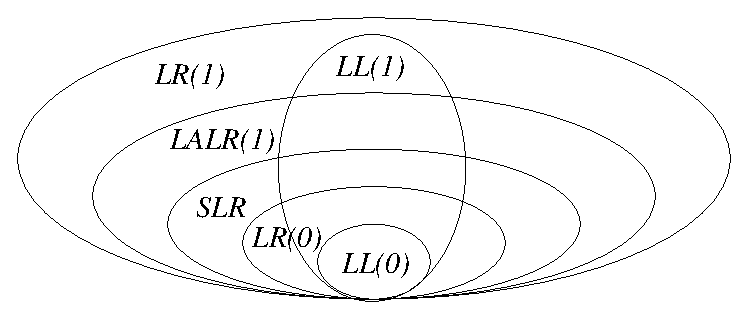
\epsfig{file = grammar_hierarchy.eps, width = 12cm}
\end{center}
\caption{La relazione fra le tecniche di parsing e le classi di grammatica
         considerate.}
  \label{fig:all_classes}
\end{figure}

Le tecniche di parsing $\mathit{LR}(0)$, $\mathit{LR}(1)$ ed
$\mathit{LALR}(1)$ si possono generalizzare a tecniche di parsing che
guardano fino a $k$ caratteri davanti alla testina di lettura dell'automa
a pila, con $k\ge 0$. Ne segue che esiste una \emph{gerarchia} di
tecniche di parsing (e conseguentemente di grammatiche da esse riconosciute).
\`E dimostrabile che ogni grammatica $\mathit{LL}(k)$ \`e anche
$\mathit{LR}(k)$, per ogni $k\ge 0$, e che il viceversa non \`e vero.
La Figura~\ref{fig:all_classes} mostra la relazione fra le classi
di parsing con $0\le k\le 1$. Si noti che $\mathit{LALR(0)}=\mathit{LR}(0)$.
Va osservato inoltre che tutte le classi di grammatica fin qui considerate
sono fatte da grammatiche non ambigue. Conseguentemente, nessuna tecnica di
parsing fra quelle viste sar\`a applicabile a una grammatica ambigua.
L'ambiguit\`a si traduce infatti in conflitti nella tabella
e solo una discesa ricorsiva non deterministica oppure
un automa a pila non deterministico potrebbero seguire al contempo
le annotazioni contrastanti della tabella. Ma tali tecniche sarebbero
troppo costose in termini computazionali.

Il parsing $\mathit{LALR}(1)$ \`e considerato come il metodo \emph{ideale} di
parsing, \nec troppo costoso \nec troppo impreciso. Per questo motivo esso
\`e implementato da JavaCup. Va detto che JavaCup costruisce
\emph{direttamente}
l'automa $\mathit{LALR}(1)$, senza passare per la semplificazione dell'automa
$\mathit{LR}(1)$, evitando quindi l'esplosione combinatoria degli stati per la
costruzione dell'automa intermedio $\mathit{LR}(1)$.
Non ci occupiamo comunque qui di questa ottimizzazione.

\`E importante invece discutere come si comporta JavaCup se nella
costruzione della tabella $\mathit{LALR}(1)$ vengono incontrari dei
conflitti, situazione non desiderabile ma che purtroppo si verifica
spesso in pratica. JavaCup usa in tal caso un sistema di \emph{risoluzione}
dei conflitti che consiste nello scegliere una delle annotazioni contrastanti
della tabella. Va subito osservato che una simile tecnica
in genere restringe l'insieme
degli alberi di parsing riconosciuti dall'automa e quindi pu\`o potenzialmente
cambiare il linguaggio da esso riconosciuto o forzare un'interpretazione
piuttosto che un'altra nel caso di grammatiche ambigue. Comunque sia,
JavaCup risolve i conflitti sposta/riduci in favore dello spostamento e i
conflitti riduci/riduci in favore della riduzione per la produzione che
appare prima nella grammatica.

Le scelte di risoluzione dei conflitti incontrati durante la generazione
di un parser vengono enumerate da JavaCup
nel file di log \texttt{syntactical/Kitten.err}, insieme agli stati dell'automa
$\mathit{LALR}(1)$ e alle relative transizioni. Tale file andrebbe quindi
sempre controllato dopo la generazione di un parser. \`E possibile specificare
un numero massimo di risoluzioni accettabili da JavaCup, superato il quale
la creazione del parser non \`e effettuata.
%
\subsection{Il parsing $\mathit{LR}$ con grammatiche ambigue}
  \label{subsec:ambiguity}
%
Abbiamo osservato che nessuna grammatica ambigua pu\`o essere
processata con uno dei metodi di parsing gi\`a visti. Abbiamo anche
detto che \`e spesso possibile trovare grammatiche non ambigue
equivalenti, ma che esse sono tipicamente complesse e innaturali
(Sezione~\ref{subsec:priorities}). In questa sezione riconsideriamo il
problema partendo dalla grammatica in Figura~\ref{fig:expressions_ambiguity}
che esprime in piccolo i problemi di ambiguit\`a della grammatica per le
espressioni Kitten vista nella Sezione~\ref{subsec:expressions_specification}.
La Figura~\ref{fig:ambiguity_automaton} mostra l'automa
$\mathit{LR}(1)$ per la grammatica in Figura~\ref{fig:expressions_ambiguity}.
Conseguentemente la sua tabella $\mathit{LR}(1)$ \`e la seguente, in cui
sono evidenti molti conflitti:
%
\begin{figure}[t]
\begin{align*}
  0)\ \ \ \ \ \,I &\to \mathit{exp}\ \mathtt{\$}\\
  1)\ \ \mathit{exp} &\to\mathit{exp}\ \mathtt{PLUS}\ \mathit{exp}\\
  2)\ \ \mathit{exp} &\to \mathit{exp}\ \mathtt{TIMES}\ \mathit{exp}\\
  3)\ \ \mathit{exp} &\to \mathtt{INTEGER}
\end{align*}
\caption{Una grammatica ambigua per le espressioni aritmetiche.}
  \label{fig:expressions_ambiguity}
\end{figure}
%
\begin{figure}[t]
\[
{\scriptsize
\xymatrix{
  \fbox{$\begin{array}{rlr}
    \mathit{exp}&\to\mathit{exp}\ \mathtt{TIMES}\ \mathit{exp}\idot &
      \{\mathtt{\$},\mathtt{PLUS},\mathtt{TIMES}\}\\
    \mathit{exp}&\to\mathit{exp}\idot\ \mathtt{PLUS}\ \mathit{exp} &
      \{\mathtt{\$},\mathtt{PLUS},\mathtt{TIMES}\}\\
    \mathit{exp}&\to\mathit{exp}\idot\ \mathtt{TIMES}\ \mathit{exp} &
      \{\mathtt{\$},\mathtt{PLUS},\mathtt{TIMES}\}
  \end{array}$}^{\ 1}\ar@/_35ex/[ddd]_(.8){\mathtt{TIMES}}
    \ar@/^/[rd]^{\mathtt{PLUS}}
  \\
  \fbox{$\begin{array}{rlr}
    \mathit{exp}&\to\mathit{exp}\ \mathtt{PLUS}\ \mathit{exp}\idot &
      \{\mathtt{\$},\mathtt{PLUS},\mathtt{TIMES}\}\\
    \mathit{exp}&\to\mathit{exp}\idot\ \mathtt{PLUS}\ \mathit{exp} &
      \{\mathtt{\$},\mathtt{PLUS},\mathtt{TIMES}\}\\
    \mathit{exp}&\to\mathit{exp}\idot\ \mathtt{TIMES}\ \mathit{exp} &
      \{\mathtt{\$},\mathtt{PLUS},\mathtt{TIMES}\}
  \end{array}$}^{\ 2}\ar@/_22ex/[dd]^(.3){\mathtt{TIMES}}
    \ar@/^3ex/[r]^{\mathtt{PLUS}}
  &
  \fbox{$\begin{array}{rlr}
    \mathit{exp}&\to\mathit{exp}\ \mathtt{PLUS}\idot\ \mathit{exp} &
      \{\mathtt{\$},\mathtt{PLUS},\mathtt{TIMES}\}\\
    \mathit{exp}&\to\idot\mathit{exp}\ \mathtt{PLUS}\ \mathit{exp} &
      \{\mathtt{\$},\mathtt{PLUS},\mathtt{TIMES}\}\\
    \mathit{exp}&\to\idot\mathit{exp}\ \mathtt{TIMES}\ \mathit{exp} &
      \{\mathtt{\$},\mathtt{PLUS},\mathtt{TIMES}\}\\
    \mathit{exp}&\to\idot\mathtt{INTEGER} &
      \{\mathtt{\$},\mathtt{PLUS},\mathtt{TIMES}\}
  \end{array}$}^{\ 3}\ar@/^3ex/[l]^{\mathit{exp}}\ar@/^/[ld]_{\mathtt{INTEGER}}
  \\
  \fbox{$\begin{array}{rlr}
    \mathit{exp}&\to\mathtt{INTEGER}\idot &
      \{\mathtt{\$},\mathtt{PLUS},\mathtt{TIMES}\}
  \end{array}$}^{\ 4}
  &
  \fbox{$\begin{array}{rlr}
    I&\to\idot\mathit{exp}\ \mathtt{\$}\\
    \mathit{exp}&\to\idot\mathit{exp}\ \mathtt{PLUS}\ \mathit{exp} &
      \{\mathtt{\$},\mathtt{PLUS},\mathtt{TIMES}\}\\
    \mathit{exp}&\to\idot\mathit{exp}\ \mathtt{TIMES}\ \mathit{exp} &
      \{\mathtt{\$},\mathtt{PLUS},\mathtt{TIMES}\}\\
    \mathit{exp}&\to\idot\mathtt{INTEGER} &
      \{\mathtt{\$},\mathtt{PLUS},\mathtt{TIMES}\}
  \end{array}$}^{\ 0}\ar[l]^{\mathtt{INTEGER}}\ar[d]^{\mathit{exp}}
  \\
  \fbox{$\begin{array}{rlr}
    \mathit{exp}&\to\mathit{exp}\ \mathtt{TIMES}\idot\ \mathit{exp} &
      \{\mathtt{\$},\mathtt{PLUS},\mathtt{TIMES}\}\\
    \mathit{exp}&\to\idot\mathit{exp}\ \mathtt{PLUS}\ \mathit{exp} &
      \{\mathtt{\$},\mathtt{PLUS},\mathtt{TIMES}\}\\
    \mathit{exp}&\to\idot\mathit{exp}\ \mathtt{TIMES}\ \mathit{exp} &
      \{\mathtt{\$},\mathtt{PLUS},\mathtt{TIMES}\}\\
    \mathit{exp}&\to\idot\mathtt{INTEGER} &
      \{\mathtt{\$},\mathtt{PLUS},\mathtt{TIMES}\}
  \end{array}$}^{\ 5}\ar@/^31ex/[uuu]_(.5){\mathit{exp}}
    \ar[u]^{\mathtt{INTEGER}}
  &
  \fbox{$\begin{array}{rlr}
    I&\to\mathit{exp}\idot\ \mathtt{\$}\\
    \mathit{exp}&\to\mathit{exp}\idot\ \mathtt{PLUS}\ \mathit{exp} &
      \{\mathtt{\$},\mathtt{PLUS},\mathtt{TIMES}\}\\
    \mathit{exp}&\to\mathit{exp}\idot\ \mathtt{TIMES}\ \mathit{exp} &
      \{\mathtt{\$},\mathtt{PLUS},\mathtt{TIMES}\}
  \end{array}$}^{\ 6}\ar@/_26ex/[uu]_(.7){\mathtt{PLUS}}
    \ar[l]^{\mathtt{TIMES}}
}}
\]
\caption{L'automa $\mathit{LR}(1)$ per la grammatica in Figura~\ref{fig:expressions_ambiguity}.}\label{fig:ambiguity_automaton}
\end{figure}
%
\begin{equation}\label{tab:expressions_conflicts}
\begin{array}{c||c|c|c|c||c|c|}
  & \mathtt{\$} & \mathtt{PLUS} & \mathtt{TIMES} & \mathtt{INTEGER} & I  & \mathit{exp}\\\hline\hline
0 &             &     &     & s4   &    & g6 \\\hline
1 & r2          & s3/r2 & s5/r2 &      &    &    \\\hline
2 & r1          & s3/r1 & s5/r1 &      &    &    \\\hline
3 &             &     &     & s4   &    & g2 \\\hline
4 & r3          & r3  & r3  &      &    &    \\\hline
5 &             &     &     & s4   &    & g1 \\\hline
6 & a           & s3  & s5  &      &    &    \\\hline
\end{array}
\end{equation}

C'\`e un conflitto sposta/riduci
nello stato $1$, di fronte al token \texttt{PLUS}, poich\'e
possiamo sia spostarci nello stato $3$ che ridurre secondo la produzione
$\mathit{exp}\to\mathit{exp}\ \mathtt{TIMES}\ \mathit{exp}$. L'item
$\mathit{exp}\to\mathit{exp}\ \mathtt{TIMES}\ \mathit{exp}\idot$ nello
stato $1$ ci dice che in tale stato abbiamo finito di leggere dal file
sorgente qualcosa che \`e il prodotto di due espressioni $\mathit{exp}_1$
ed $\mathit{exp}_2$. Ridurre secondo
la produzione $\mathit{exp}\to\mathit{exp}\ \mathtt{TIMES}\ \mathit{exp}$
significherebbe quindi vedere tale prodotto come un'unica espressione il cui
risultato \`e sommato con quel che segue.
Spostare il token $\mathtt{PLUS}$ significherebbe considerare
$\mathit{exp}_2$ come l'inizio di una addizione, il cui risultato deve
essere poi moltiplicato per $\mathit{exp}_1$. \`E qui evidente che
ci scontriamo contro l'ambiguit\`a della grammatica. Ridurre secondo la
produzione $\mathit{exp}\to\mathit{exp}\ \mathtt{TIMES}\ \mathit{exp}$
significa dare priorit\`a alla moltiplicazione, mentre spostare
$\mathtt{PLUS}$ significa dare priorit\`a all'addizione. La scelta ragionevole
\`e quindi quella di risolvere l'ambiguit\`a riducendo secondo la produzione
$\mathit{exp}\to\mathit{exp}\ \mathtt{TIMES}\ \mathit{exp}$. In termini della
tabella $\mathit{LR}(1)$, questo significa che nello sttao $1$, di fronte
a $\mathtt{PLUS}$, risolviamo il conflitto
lasciando l'azione di riduzione ed eliminado l'azione di spostamento del token.
Un ragionamento simile ci fa concludere che nello stato $2$,
di fronte al token $\mathtt{TIMES}$, preferiamo spostare il token
piuttosto che ridurre secondo la produzione
$\mathit{exp}\to\mathit{exp}\ \mathtt{PLUS}\ \mathit{exp}$.

Un altro conflitto sorge ancora nello stato $1$ di fronte al token
$\mathtt{TIMES}$. In tale stato abbiamo gi\`a letto dei token che formano
la moltiplicazione di due espressioni $\mathit{exp}_1$ ed $\mathit{exp}_2$.
Abbiamo sia la possibilit\`a di ridurre secondo la produzione
$\mathit{exp}\to\mathit{exp}\ \mathtt{TIMES}\ \mathit{exp}$ che
di spostare il token $\mathtt{TIMES}$
e andare nello stato $5$. La prima scelta significa
legare il prodotto di $\mathit{exp}_1$ ed $\mathit{exp}_2$
riducendolo a un'espressione moltiplicata per
quel che segue il $\mathtt{TIMES}$, mentre la seconda scelta considera
$\mathit{exp}_2$ come l'inizio di un prodotto il cui risultato
viene moltiplicato per $\mathit{exp}_1$. Dal momento che preferiamo una
associativit\`a a sinistra per la moltiplicazione, facciamo la scelta di
ridurre secondo la produzione
$\mathit{exp}\to\mathit{exp}\ \mathtt{TIMES}\ \mathit{exp}$.
Similmente nello stato $2$ di fronte al token $\mathtt{PLUS}$ preferiamo
ridurre secondo la produzione
$\mathit{exp}\to\mathit{exp}\ \mathtt{PLUS}\ \mathit{exp}$ piuttosto
che spostare e andare nello stato $3$. Ecco quindi che la
tabella~\eqref{tab:expressions_conflicts}
viene semplificata in una tabella senza conflitti:
%
\[
\begin{array}{c||c|c|c|c||c|c|}
  & \mathtt{\$} & \mathtt{PLUS} & \mathtt{TIMES} & \mathtt{INTEGER} & I  & \mathit{exp}\\\hline\hline
0 &             &     &     & s4   &    & g6 \\\hline
1 & r2          & r2 & r2 &      &    &    \\\hline
2 & r1          & r1 & s5 &      &    &    \\\hline
3 &             &     &     & s4   &    & g2 \\\hline
4 & r3          & r3  & r3  &      &    &    \\\hline
5 &             &     &     & s4   &    & g1 \\\hline
6 & a           & s3  & s5  &      &    &    \\\hline
\end{array}
\]
che implementa il parsing delle espressioni aritmetiche con le
usuali regole di precedenza e associativit\`a.

La specifica della precedenza e dell'associativit\`a degli operatori
aritmetici viene fatta in JavaCup con le direttive che abbiamo visto nella
Sezione~\ref{subsec:priorities}, le quali modificano il comportamento
di JavaCup nella risoluzione dei conflitti (Sezione~\ref{subsec:lalr1}).
Una direttiva \texttt{precedence xxx $t$} d\`a infatti al token $t$ una
priorit\`a maggiore di quella di tutti gli altri token enumerati dalle
direttive precedenti. Inoltre essa d\`a alle produzioni il cui ultimo
token a destra \`e $t$ una priorit\`a pari a quella di $t$. Un conflitto
sposta/riduci viene a questo punto risolto preferendo lo spostamento se il
token spostato ha priorit\`a maggiore della produzione per cui si dovrebbe
ridurre; la riduzione nel caso opposto. Conseguentemente, con le direttive
della Sezione~\ref{subsec:priorities} fra una riduzione per
$\mathit{exp}\to\mathit{exp}\ \mathtt{TIMES}\ \mathit{exp}$ e lo spostamento
di un $\mathtt{PLUS}$ si preferisce la riduzione. A parit\`a di
priorit\`a si seguono le direttive di associativit\`a preferendo la
riduzione se l'associativit\`a \`e \texttt{left}, lo spostamento
se l'associativit\`a \`e \texttt{right} e lasciando la casella vuota
se l'associativit\`a \`e \texttt{nonassoc}, in modo da segnalare un errore
in tale situazione.

Un altro problema di ambiguit\`a della grammatica Kitten (e in genere di
tutti i linguaggi imperativi) \`e relativo
all'\texttt{if/then/else}, in cui il ramo \texttt{else} \`e normalmente
facoltativo. Ne consegue che nel caso di \texttt{if} annidati risulta ambigua
l'associazione degli \texttt{else} all'\texttt{if} da cui dipendono.
Questo problema \`e tipicamente risolto associando
ogni \texttt{else} all'ultimo \texttt{then} incontrato. Per esempio,
vogliamo che
\texttt{if (a > 5) then if (b < 4) then a := 3 else b := 6}
venga interpretato come
\texttt{if (a > 5) then \{if (b < 4) then a := 3 else b := 6\}}
piuttosto che come
\texttt{if (a > 5) then \{if (b < 4) then a := 3\} else b := 6}.
A tal fine il parser, di fronte all'ultimo token \texttt{ELSE},
deve spostare tale token piuttosto che ridurre secondo la produzione
%
\begin{verbatim}
  exp ::= IF LPAREN exp RPAREN THEN command
\end{verbatim}
%
della Sezione~\ref{subsec:commands_specification}.
Abbiamo detto nella Sezione~\ref{subsec:lalr1} che
JavaCup risolve un conflitto sposta/riduci in favore dello spostamento,
che \`e quello che volevamo, e annotando nel
file \texttt{syntactical/Kitten.err} che il conflitto \`e stato risolto in
tal senso. Per evitare tale annotazione (essenzialmente un \emph{warning})
e non contare questa risoluzione nel novero di quelle ammesse al massimo
da JavaCup, basta dichiarare esplicitamente che l'\texttt{ELSE} ha priorit\`a
rispetto al \texttt{THEN}. Otteniamo questo effetto aggiungendo al file
\texttt{syntactical/Kitten.cup} le dichiarazioni:
%
\begin{verbatim}
  precedence nonassoc THEN;
  precedence nonassoc ELSE;
\end{verbatim}
%
la cui annotazione di associativit\`a \`e irrilevante.
Un simile problema si presenta fra gli operatori di confronto e i token
\texttt{DOT} e \texttt{LBRACK}, risolto in modo simile (si veda la
Sezione~\ref{subsec:priorities}).

Un altro problema di ambiguit\`a della grammatica Kitten della
Sezione~\ref{sec:java_cup} \`e legato al meno unario. L'espressione
$\mathtt{MINUS}\ \mathit{exp}\ \mathtt{PLUS}\ \mathit{exp}$ pu\`o
essere interpretata sia come
$\mathtt{MINUS}\ (\mathit{exp}\ \mathtt{PLUS}\ \mathit{exp})$ che come
$(\mathtt{MINUS}\ \mathit{exp})\ \mathtt{PLUS}\ \mathit{exp}$ e quest'ultima
\`e l'interpretazione preferita. Conseguentemente la riduzione
secondo la produzione \texttt{exp ::= MINUS exp} deve essere preferita
a qualsiasi spostamento dei token che seguono la prima espressione.
Otteniamo questo effetto dando esplicitamente una priorit\`a massima a tale
produzione:
%
\begin{verbatim}
  exp ::= MINUS exp %prec UMINUS
\end{verbatim}
%
dove il token \texttt{UMINUS} ha ricevuto una priorit\`a maggiore di qualsiasi
suo seguito (Sezione~\ref{subsec:priorities}).

Risolti questi aspetti di ambiguit\`a della grammatica Kitten, il
programma JavaCup \`e capace di generare il parser per Kitten senza
segnalare alcuna risoluzione di conflitto.

Concludiamo questa sezione ricordando che la risoluzione dei conflitti
tramite annotazioni di precedenza e associativit\`a \`e generalmente
pericolosa perch\'e si rischia di cambiare il linguaggio riconosciuto dal
parser. Essa \`e usata in letteratura limitatamente ai soli esempi visti in
questa sezione.
%
\section{Le azioni semantiche e la costruzione induttiva della sintassi astratta}\label{sec:abstract_syntax}
%
La grammatica Kitten della Sezione~\ref{sec:java_cup} specifica
quali stringhe (\emph{file sorgenti}) appartengono al linguaggio Kitten.
Il parser generato da JavaCup si limita quindi a riconoscere le stringhe
del linguaggio. JavaCup ammette per\`o la possibilit\`a di \emph{decorare}
la grammatica con delle \emph{azioni semantiche} che vengono eseguite
in corrispondenza alle azioni di riduzione della tabella $\mathit{LALR}(1)$.
Tali azioni semantiche possono essere usate per molti scopi. In questa
sezione vediamo alcuni esempi.

Riconsideriamo la grammatica in Figura~\ref{fig:grammar_lists}, che in
JavaCup \`e scritta come
%
\begin{verbatim}
  terminal a b;
  non terminal L A B;

  start with L;

  L ::= A B ;
  A ::=
   | a A ;
  B ::=
   | b B ;
\end{verbatim}
%
Supponiamo di voler sapere, per ogni file sorgente, non solo se esso
soddisfa la grammatica, cio\`e se esso \`e formato da una lista di
\texttt{a} seguita da una lista di \texttt{b}, ma anche la lunghezza delle
due liste. A tal fine decidiamo che il non terminale $A$ deve conoscere
quante \texttt{a} sono state derivate da esso e il non terminale $B$
quante \texttt{b} sono state derivate da esso. Diciamo che il
\emph{valore semantico} del non terminale $A$ \`e il numero di \texttt{a}
da esso derivate e il valore semantico del non terminale $B$ \`e il numero
di \texttt{b} da esso derivate. I valori semantici vanno dichiarati nella
enumerazione dei non terminali. Dal momento che nel nostro caso si tratta
di valori interi, scriveremo\footnote{Il valore semantico in JavaCup deve
in effetti essere un oggetto, per cui non \`e possibile utilizzare il tipo
primitivo \texttt{int} ma occorrerebbe far ricorso alla classe involucro
\texttt{java.lang.Integer}. \`E solo per semplicit\`a espositiva che preferiamo
utilizzare nei nostri esempi il tipo \texttt{int}.}
%
\begin{verbatim}
  non terminal int A;
  non terminal int B;
\end{verbatim}
%
A questo punto dobbiamo specificare come si calcolano tali valori semantici.
Il calcolo avviene
\emph{decorando} ciascuna produzione per $A$ con delle \emph{azioni semantiche}
che specificano il valore semantico di $A$ per ciascuna delle sue due
produzioni. Similmente per $B$:
%
\begin{verbatim}
  A ::=
     {: RESULT = 0; :}
   | a A:l
     {: RESULT = 1 + l; :} ;

  B ::=
     {: RESULT = 0; :}
   | b B:l
     {: RESULT = 1 + l; :} ;
\end{verbatim}
%
Le azioni semantiche sono codice Java che si aggiunge dopo ciascuna produzione,
racchiuso fra i delimitatori \verb!{:! e \verb!:}!. Tale codice calcola
il valore semantico \texttt{RESULT} usando i valori semantici dei componenti
dei lati destri delle produzioni. Nell'esempio sopra diciamo che se una
lista di \texttt{a} \`e vuota allora il numero di \texttt{a}
incontrate \`e $0$. Se una lista di \texttt{a} \`e invece fatta da una
\texttt{a} seguita da $l$ \texttt{a}, il numero complessivo di \texttt{a}
incontrate \`e $1 + l$. Un ragionamento simile si applica per $B$.
Si noti che abbiamo \emph{decorato} dei non terminali alla destra delle
produzioni facendoli seguire da un carattere due punti e da una variabile
che contiene il loro valore semantico. \`E possibile decorare anche i terminali
che stanno alla destra di una produzione. Il valore semantico dei terminali
\`e per definizione il loro valore lessicale (Capitolo~\ref{chap:lexical})
che normalmente \`e \texttt{null} tranne se l'analizzatore lessicale
ha sintettizato per essi un apposito valore lessicale, come avviene in Kitten
per gli identificatori, le stringhe e le costanti numeriche.

Continuando il nostro esempio, il numero di \texttt{a} e il numero di
\texttt{b} incontrate nel file sorgente vanno fatti risalire fino al
non terminale iniziale. Dal momento che si tratta di \emph{due} interi,
siamo costretti a definire una struttura dati composta da due campi
di tipo \texttt{int}:
%
\begin{verbatim}
  public class Pair {
    private int a;
    private int b;

    public Pair(int a, int b) {
      this.a = a;
      this.b = b;
    }
  }
\end{verbatim}
%
Dichiariamo il tipo del valore lessicale per la $L$:
%
\begin{verbatim}
  non terminal Pair L;
\end{verbatim}
%
quindi specifichiamo come si costruisce tale valore lessicale:
%
\begin{verbatim}
  L ::= A:a B:b
      {: RESULT = new Pair(a,b); :} ;
\end{verbatim}
%
La grammatica decorata \`e in Figura~\ref{fig:grammar_lists_decoration}.
Il valore semantico del non terminale iniziale \`e poi ritornato
come valore di ritorno del metodo \texttt{parse()} della classe
\texttt{Parser} che viene generata da JavaCup
(Sezione~\ref{subsec:jlex_and_java_cup}).
%
\begin{figure}[t]
\begin{verbatim}
                       terminal a b;
                       non terminal int A;
                       non terminal int B;
                       non terminal Pair L;
                       start with L;

                       L ::= A:a B:b
                            {: RESULT = new Pair(a,b); :} ;

                       A ::=
                            {: RESULT = 0; :}
                         | a A:l
                            {: RESULT = 1 + l; :} ;

                       B ::=
                            {: RESULT = 0; :}
                         | b B:l
                            {: RESULT = 1 + l; :} ;
\end{verbatim}
\caption{La grammatica di Figura~\ref{fig:grammar_lists} decorata con delle
         azioni semantiche che calcolano il numero di \texttt{a} e il numero
         di \texttt{b} incontrate nel file sorgente.}
  \label{fig:grammar_lists_decoration}
\end{figure}

L'implementaziome delle azioni semantiche \`e basata su una semplice
modifica dell'automa a pila della Sezione~\ref{sec:lr}. Oltre a utilizzare
uno stack di stati, l'automa a pila utilizza adesso anche uno stack di
valori semantici, corrispondenti ai terminali o non terminali che sono
stati spostati o a cui si \`e ridotto per ottenere lo stato
nella posizione corrispondente dello stack di stati.
Tale stack di valori semantici \`e in effetti implementato da JavaCup come
uno stack di \texttt{java\_cup.runtime.Symbol}
(Figura~\ref{fig:java_cup.runtime.Symbol}). Il campo \texttt{value} \`e
utilizzato proprio per contenere il valore semantico ed \`e accessibile
tramite la variabile $v$ che si dichiara nella notazione
$\mathit{terminale}:v$ o $\mathit{non\ terminale}:v$.

Simuliamo per esempio
il comportamento dell'automa a pila di fronte alla stringa
$\mathtt{aab\$}$, utilizzando la tabella~\eqref{tab:slr_grammar_lists} e le
azioni semantiche in Figura~\ref{fig:grammar_lists_decoration}.
Indicando con $/$ il valore semantico $\mathtt{null}$, la
configurazione iniziale dell'automa \`e:
%
\begin{align*}
  0 & & \mathtt{aab\$}\\
  / & &
\end{align*}
%
dove il valore semantico $/$ per lo stato $0$ \`e irrilevante. A questo
punto, di fronte al lookahead \texttt{a}, la
tabella~\eqref{tab:slr_grammar_lists} ci dice di andare nello stato $2$.
Dal momento che il valore semantico dei token \`e per default
$\mathtt{null}$, otteniamo la configurazione
%
\begin{align*}
  0,2 & & \mathtt{ab\$}\\
  /,/ & &
\end{align*}
%
Nello stato $2$ di fronte al lookahead \texttt{a} restiamo in $2$:
%
\begin{align*}
  0,2,2 & & \mathtt{b\$}\\
  /,/,/ & &
\end{align*}
%
mentre di fronte al lookahead \texttt{b} riduciamo secondo la
produzione $A\to\varepsilon$ e poi andiamo nello stato $5$.
La produzione \`e stata decorata in modo tale che il
valore semantico della $A$ \`e $0$. La configurazione risultante \`e quindi:
%
\begin{align*}
  0,2,2,5 & & \mathtt{b\$}\\
  /,/,/,0 & &
\end{align*}
%
Nello stato $5$ di fronte al lookahead \texttt{b} riduciamo secondo
la produzione $A\to\mathtt{a}A$ per cui dobbiamo levare due stati dallo
stack e sostituirli con lo stato $5$. Gli ultimi due elementi dello stack
dei valori semantici sono $/$ e $0$ per cui nella
Figura~\ref{fig:grammar_lists_decoration} il valore di $l$ \`e $0$.
Conseguentemente il valore semantico $1+l$ \`e pari ad $1$ e otteniamo la
configurazione:
%
\begin{align*}
  0,2,5 & & \mathtt{b\$}\\
  /,/,1 & &
\end{align*}
%
Dobbiamo nuovamente ridurre secondo la produzione $A\to\mathtt{a}A$ ottenendo
questa volta:
%
\begin{align*}
  0,3 & & \mathtt{b\$}\\
  /,2 & &
\end{align*}
%
Nello stato $3$ di fronte al lookahead \texttt{b} finiamo nello stato $6$:
%
\begin{align*}
  0,3,6 & & \mathtt{\$}\\
  /,2,/ & &
\end{align*}
%
e nello stato $6$ di fronte al lookahead $\mathtt{\$}$ riduciamo secondo la
produzione $B\to\varepsilon$ per cui otteniamo la configurazione
%
\begin{align*}
  0,3,6,7 & & \mathtt{\$}\\
  /,2,/,0 & &
\end{align*}
%
Nello stato $7$ di fronte al lookahead $\mathtt{\$}$ riduciamo secondo la
produzione $B\to\mathtt{b}B$ per cui dobbiamo eliminare due stati dallo stack
e sostituirli con lo stato $4$. Inoltre avremo $l=0$ in
Figura~\ref{fig:grammar_lists_decoration} e conseguentemente otteniamo la
configurazione:
%
\begin{align*}
  0,3,4 & & \mathtt{\$}\\
  /,2,1 & &
\end{align*}
%
Nello stato $4$ di fronte al lookahead $\mathtt{\$}$ dobbiamo ridurre
secondo la produzione $L\to AB$ per cui dobbiamo eliminare due
stati dallo stack e sostituirli con lo stato $1$. In
Figura~\ref{fig:grammar_lists_decoration} avremo $a=2$ e $b=1$ per cui
otteniamo la configurazione
%
\begin{align*}
  0,1 & & \mathtt{\$}\\
  /,p & &
\end{align*}
%
dove $p$ \`e un puntatore in memoria a un oggetto \texttt{Pair} i cui campi
\texttt{a} e \texttt{b} contengono rispettivamente $2$ e $1$.
A questo punto l'automa si ferma accettando la stringa $\mathtt{aab\$}$
poich\'e nello stato $1$ di fronte al lookahead $\mathtt{\$}$ la
tabella~\ref{tab:slr_grammar_lists} richiede di accettare il file sorgente.

Consideriamo un altro esempio di decorazione di una grammatica
con azioni semantiche. La grammatica in
Figura~\ref{fig:expressions_ambiguity} specifica delle espressioni aritmetiche
su interi. Supponiamo che l'analizzatore lessicale associ al token
\texttt{INTEGER} il valore numerico concreto presente nel file
sorgente (Capitolo~\ref{chap:lexical}). Le azioni semantiche in
Figura~\ref{fig:expressions_decoration} calcolano il valore dell'espressione
contenuta nel file sorgente. Si noti che se l'espressione \`e formata
semplicemente da un numero intero allora la produzione decorata
%
\begin{verbatim}
  exp ::= INTEGER:i
       {: RESULT = i; :} ;
\end{verbatim}
%
usa il valore lessicale del token \texttt{INTEGER} per sintetizzare il
valore semantico di \texttt{exp}. In tal caso occorre dichiarare
qual \`e il valore lessicale di \texttt{INTEGER}, con la dichiarazione
%
\begin{verbatim}
  terminal int INTEGER;
\end{verbatim}
%
Tale dichiarazione deve essere compatibile con il tipo del valore
lessicale effettivamente calcolato dall'analizzatore lessicale per il token
\texttt{INTEGER}.

\begin{figure}[t]
\begin{verbatim}
                       terminal PLUS, TIMES;
                       terminal int INTEGER;
                       non terminal int exp;
                       start with exp;

                       exp ::=
                           exp:e1 PLUS exp:e2
                             {: RESULT = e1 + e2; :}
                         | exp:e1 TIMES exp:e2
                             {: RESULT = e1 * e2; :}
                         | INTEGER:i
                             {: RESULT = i; :} ;
\end{verbatim}
\caption{La grammatica di Figura~\ref{fig:expressions_ambiguity}
         decorata con delle
         azioni semantiche che calcolano il valore dell'espressione di cui
         il file sorgente \`e composto.}
  \label{fig:expressions_decoration}
\end{figure}

\begin{exercise}\label{ex:decoration1}
Si scriva una grammatica non ambigua che genera il linguaggio delle
stringhe di \texttt{a} e \texttt{b}. Quindi la si decori con delle
azioni semantiche che calcolano la differenza fra il numero delle \texttt{a}
e il numero delle \texttt{b}.
\end{exercise}
%
\begin{exercise}\label{ex:decoration2}
Supponendo che il token \texttt{INTEGER} rappresenti solo numeri interi
maggiori o uguali a $0$, si decori la grammatica della
Figura~\ref{fig:expressions_ambiguity} con delle azioni semantiche che
calcolano un valore booleano. Tale valore deve essere \textit{true}
se e solo se il valore dell'espressione non \`e $0$.
\end{exercise}

Un'applicazione delle azioni semantiche \`e la creazione, durante il
parsing, della \emph{sintassi astratta}
del codice sorgente, cio\`e di un albero,
come quello della Figura~\ref{fig:led_albero}, che descrive la \emph{struttura
logica} del codice. L'idea \`e quella di fare
sintetizzare a ciascun non terminale, come valore semantico, la sintassi
astratta della parte di codice da esso derivata.

\begin{figure}[t]
\begin{verbatim}
                       terminal a b;
                       non terminal AbstractA A;
                       non terminal AbstractB B;
                       non terminal AB L;
                       start with L;

                       L ::= A:a B:b
                            {: RESULT = new AB(a,b); :} ;

                       A ::=
                            {: RESULT = new EmptyA(); :}
                         | a A:l
                            {: RESULT = new OneA(l); :} ;

                       B ::=
                            {: RESULT = new EmptyB(); :}
                         | b B:l
                            {: RESULT = new OneB(l); :} ;
\end{verbatim}
\caption{La grammatica di Figura~\ref{fig:grammar_lists} decorata con delle
         azioni semantiche che sintetizzano la sua sintassi astratta.}
  \label{fig:grammar_lists_abstract_syntax}
\end{figure}

Supponiamo per esempio di volere generare la sintassi astratta per la
grammatica in Figura~\ref{fig:grammar_lists}, modificando le azioni semantiche
della Figura~\ref{fig:grammar_lists_decoration}. Otteniamo la grammatica
decorata in Figura~\ref{fig:grammar_lists_abstract_syntax}.
La classe \texttt{EmptyB} rappresenta una sequenza vuota di \texttt{b}.
La classe \texttt{OneB} rappresenta invece una \texttt{b} seguita da una
sequenza di \texttt{b}. Dal momento che dobbiamo assegnare \emph{un} tipo
al valore semantico sintetizzato per \texttt{B}, tali due classi devono
essere sottoclassi di una classe \texttt{AbstractB} che denota
genericamente delle sequenze di \texttt{b}. Tale classe \`e bene che
sia lasciata astratta, nel senso di Java:
%
\begin{verbatim}
  public abstract class AbstractB {}

  public class EmptyB extends AbstractB {}

  public class OneB extends AbstractB {
    private AbstractB l;
    public OneB(AbstractB l) { this.l = l; }
  }
\end{verbatim}
%
Identica \`e l'impostazione delle classi \texttt{EmptyA},
\texttt{OneA} e \texttt{AbstractA}. La classe \texttt{AB} \`e invece definita
come:
%
\begin{verbatim}
  public class AB {
    private AbstractA a;
    private AbstractB b;
    public AB(AbstractA a, AbstractB b) { this.a = a; this.b = b; }
  }
\end{verbatim}
%
dal momento che c'\`e solo una produzione per \texttt{L}.

Si noti l'estrema \emph{arbitrariet\`a} della rappresentazione
della sintassi astratta. Per esempio, un'altra possibile organizzazione
della sintassi astratta per la grammatica in Figura~\ref{fig:grammar_lists}
\`e mostrata in Figura~\ref{fig:grammar_lists_abstract_syntax2}.
Questa volta le classi di sintassi astratta sono implementate come
%
\begin{verbatim}
  public class ListA {
    private ListA tail;
    public ListA(ListA tail) { this.tail = tail; }
  }

  public class ListB {
    private ListB tail;
    public ListB(ListB tail) { this.tail = tail; }
  }

  public class AB {
    private ListA a;
    private ListB b;
    public AB(ListA a, ListB b) { this.a = a; this.b = b; }
  }
\end{verbatim}

Altre scelte sarebbero possibili e legittime. In genere \`e importante
che la sintassi astratta semplifichi la comprensione e l'elaborazione
del codice che essa astrae (Capitolo~\ref{chap:recursive_descent}).
Una buona euristica \`e quella di definire una classe di sintassi astratta
per ogni produzione, i cui oggetti hanno un campo per ogni non terminale
nel lato destro della produzione. Quindi si definisce una classe astratta
(nel senso di Java) che fa da superclasse a tutte le classi di sintassi
astratta per le produzioni che hanno a sinistra lo stesso non terminale. Da
questo punto di vista \`e quindi
pi\`u \emph{standard} una sintassi astratta generata come in
Figura~\ref{fig:grammar_lists_abstract_syntax} che non una generata come in
Figura~\ref{fig:grammar_lists_abstract_syntax2}.
%
\begin{figure}[t]
\begin{verbatim}
                       terminal a b;
                       non terminal ListA A;
                       non terminal ListB B;
                       non terminal AB L;
                       start with L;

                       L ::= A:a B:b
                            {: RESULT = new AB(a,b); :} ;

                       A ::=
                            {: RESULT = null; :}
                         | a A:l
                            {: RESULT = new ListA(l); :} ;

                       B ::=
                            {: RESULT = null; :}
                         | b B:l
                            {: RESULT = new ListB(l); :} ;
\end{verbatim}
\caption{La grammatica di Figura~\ref{fig:grammar_lists} decorata con delle
         azioni semantiche che sintetizzano la sua sintassi astratta
         come liste di \texttt{a} e di \texttt{b}.}
  \label{fig:grammar_lists_abstract_syntax2}
\end{figure}

\greycomment{Le azioni semantiche possono essere utilizzate per svariati
scopi. L'unico uso per cui le utilizziamo nel compilatore Kitten \`e per la
generazione della sintassi astratta del codice sorgente. Su tale sintassi
astratta definiamo poi dei metodi virtuali a discesa ricorsiva
che permettono per esempio
di effettuare il type-checking e la generazione del codice intermedio
(Capitoli~\ref{chap:semantical} e~\ref{chap:translate}). \`E possibile
comunque utilizzare le stesse azioni semantiche per svolgere
tali compiti. Questo approccio \e sicuramente pi\`u
tradizionale~\cite{AhoSU86} ma finisce per sovraccaricare il file
\texttt{syntactical/Kitten.cup} con informazione non relativa all'aspetto
sintattico
del linguaggio. Inoltre l'uso di un linguaggio a oggetti per l'implementazione
del compilatore ben si accompagna alla definizione del type-checking e della
generazione del codice intermedio tramite metodi virtuali delle classi di
sintassi astratta, permettendo per esempio di definire in maniera molto
semplice un comportamento di default per tutta una classe di strutture
sintattiche (come per gli operatori binari).}
%
\section{La sintassi astratta di Kitten}\label{sec:abstract_syntax_classes}
%
La generazione della sintassi astratta di Kitten avviene come abbiamo
visto sopra in Figura~\ref{fig:grammar_lists_abstract_syntax}.
L'idea \`e di far sintetizzare a ciascun non terminale, tramite azioni
semantiche, l'albero di sintassi astratta della parte di codice
sorgente da esso derivato.

Vediamo per esempio come modifichiamo a tal fine una delle produzioni
della Sezione~\ref{subsec:expressions_specification}:
%
\begin{verbatim}
  exp ::= exp:left PLUS:p exp:right
     {: RESULT = new Addition(pleft,left,right); :}
\end{verbatim}
%
Per induzione, \texttt{left} e \texttt{right} contengono l'albero
di sintassi astratta per la parte di codice derivata dai due addendi
dell'addizione. Invece \texttt{p} contiene il valore lessicale del
token \texttt{PLUS}, che come abbiamo gi\`a detto \`e \texttt{null}
essendo \texttt{PLUS} un terminale. Questo non significa che
la notazione \texttt{PLUS:p} sia inutile: essa dichiara implicitamente
anche una variabile \texttt{pleft} che dice quanti caratteri sono
passati dall'inizio del file sorgente fino al token \texttt{PLUS}. In pratica,
\texttt{pleft} \`e un accesso al campo \texttt{left} della struttura
dati in Figura~\ref{fig:java_cup.runtime.Symbol}.
Conservare questa informazione nell'albero astratto \`e importante nel caso
in cui, in futuro, servisse segnalare un qualche errore su questa
addizione (Capitolo~\ref{chap:lexical}).
Si noti che esistono anche le variabili \texttt{leftleft} corrispondente
a \texttt{left} e \texttt{rightleft} corrispondente a \texttt{right}, ma
in questo caso esse non sono utilizzate. Quello che stiamo
dicendo con la precedente produzione \`e quindi
che il valore semantico per una addizione \`e un
albero astratto con una radice che \`e un nodo di tipo \texttt{Addition}
e i cui due figli sono gli alberi astratti per i due addendi dell'addizione.
Inoltre la posizione in cui deve essere segnalato un eventuale errore
semantico \`e quella del token \texttt{PLUS}.

Affich\'e la definizione induttiva dell'albero astratto per un pezzo di codice
sia ben fondata, occorre che ci siano anche dei casi base. Per esempio,
un caso base \`e il seguente:
%
\begin{verbatim}
  exp ::= TRUE:t
     {: RESULT = new True(tleft); :}
\end{verbatim}
%
il quale dice che il valore semantico per la costante \texttt{true}
\`e un nodo di tipo \texttt{True}, privo di figli. Eventuali
errori su questa parte di codice devono essere in futuro segnalati
alla posizione in cui inizia l'espressione \texttt{true}, cio\`e a
\texttt{tleft} caratteri dall'inizio del file sorgente.

Le classi di sintassi astratta utilizzate
per rappresentare il codice sorgente Kitten in maniera strutturata si trovano
all'interno della directory \texttt{absyn} di Kitten.
Esse sono tutte sottoclassi della classe astratta
(nel senso di Java) \texttt{absyn/Absyn.java} mostrata in
Figura~\ref{fig:absyn.Absyn}.
Una classe di sintassi astratta ha sempre un campo \texttt{pos} che
indica dove deve essere segnalato un errore verificatosi sulla parte di codice
da essa rappresentata. La posizione \texttt{pos} viene specificata
al momento della creazione del nodo di sintassi astratta tramite le azioni
semantiche e pu\`o essere letta in seguito con il metodo \texttt{getPos()}.
Si noti che ogni nodo di sintassi
astratta ha anche un identificatore numerico unico \texttt{identifier},
la cui utilit\`a sar\`a chiara in seguito quando descriveremo la
rappresentazione grafica dell'albero di sintassi astratta
(Sezione~\ref{sec:graphical_abstract_syntax}).
%
\begin{figure}[t]
\begin{verbatim}
                     public abstract class Absyn {
                       private int pos;
                       private int identifier;
                       private static int counter = 0;

                       protected Absyn(int pos) {
                         this.pos = pos;
                         this.identifier = counter++;
                       }

                       public int getPos() {
                         return pos;
                       }
                     }
\end{verbatim}
\caption{La superclasse di tutte le classi di sintassi astratta per Kitten.}
  \label{fig:absyn.Absyn}
\end{figure}

Le espressioni sono una sottoclasse di \texttt{absyn/Absyn.java}.
Le definiamo come
%
\begin{verbatim}
  public abstract class Expression extends Absyn {
    protected Expression(int pos) {
      super(pos);
    }
  }
\end{verbatim}
%
A questo punto possiamo dire che la classe di sintassi astratta
\texttt{absyn/True.java} \`e un caso particolare di espressione:
%
\begin{verbatim}
  public class True extends Expression {
    public True(int pos) {
      super(pos);
    }
  }
\end{verbatim}
%
Si noti che questa volta si tratta di una classe concreta, nel senso di Java.

Il caso della classe di sintassi astratta \texttt{absyn/Addition.java}, che
rappresenta un'operazione binaria di addizione, \`e
pi\`u complesso. In primo luogo, definiamo le operazioni binarie come un
caso particolare delle espressioni:
%
\begin{verbatim}
  public abstract class BinOp extends Expression {
    private Expression left;
    private Expression right;

    protected BinOp(int pos, Expression left, Expression right) {
      super(pos);
      this.left = left;
      this.right = right;
    }
  }
\end{verbatim}
%
Si noti che un'operazione binaria ha due campi \texttt{left} e \texttt{right}
che sono, ricorsivamente, la sintassi astratta dei suoi due operandi.
Si noti inoltre che il costruttore inizializza la parte di stato di sua
competenza e demanda alla superclasse l'inizializzazione del resto, cio\`e in
questo caso di \texttt{pos}.
A questo punto definiamo un caso particolare di operazione binaria,
cio\`e un'operazione binaria aritmetica:
%
\begin{verbatim}
  public abstract class ArithmeticBinOp extends BinOp {
    protected ArithmeticBinOp(int pos, Expression left, Expression right) {
      super(pos,left,right);
    }
  }
\end{verbatim}
%
Siamo finalmente nelle condizioni di definire \texttt{absyn/Addition.java}
come un caso particolare di operazione binaria aritmetica:
%
\begin{verbatim}
  public class Addition extends ArithmeticBinOp {
    public Addition(int pos, Expression left, Expression right) {
      super(pos,left,right);
    }
  }
\end{verbatim}
%
Questa volta si tratta di una classe concreta, nel senso di Java.
Si osservi che le classi
astratte, nel senso di Java, hanno costruttori \texttt{protected},
utilizzabili quindi solo dalle classi concrete che le estendono,
tramite la chiamata \texttt{super} a un costruttore della superclasse.

\javatip{
La strutturazione gerarchica delle classi di sintassi astratta e l'uso
intenso di classi astratte, nel senso di Java, pu\`o non essere immediatamente
apprezzabile. Quando, per\`o, definiremo algoritmi ricorsivi sulla sintassi
astratta, ci accorgeremo che una buona strutturazione gerachica aiuta
significativamente la definizione di tali algoritmi. \`E un tipico
caso in cui l'impostazione a oggetti del codice semplifica
nettamente lo sviluppo del software.}

Vediamo adesso in maniera pi\`u dettagliata quali sono le classi di
sintassi astratta di Kitten.
%
\subsection{Le classi di sintassi astratta per i tipi}
  \label{subsec:types_abstract}
%
\begin{figure}[t]
\begin{center}
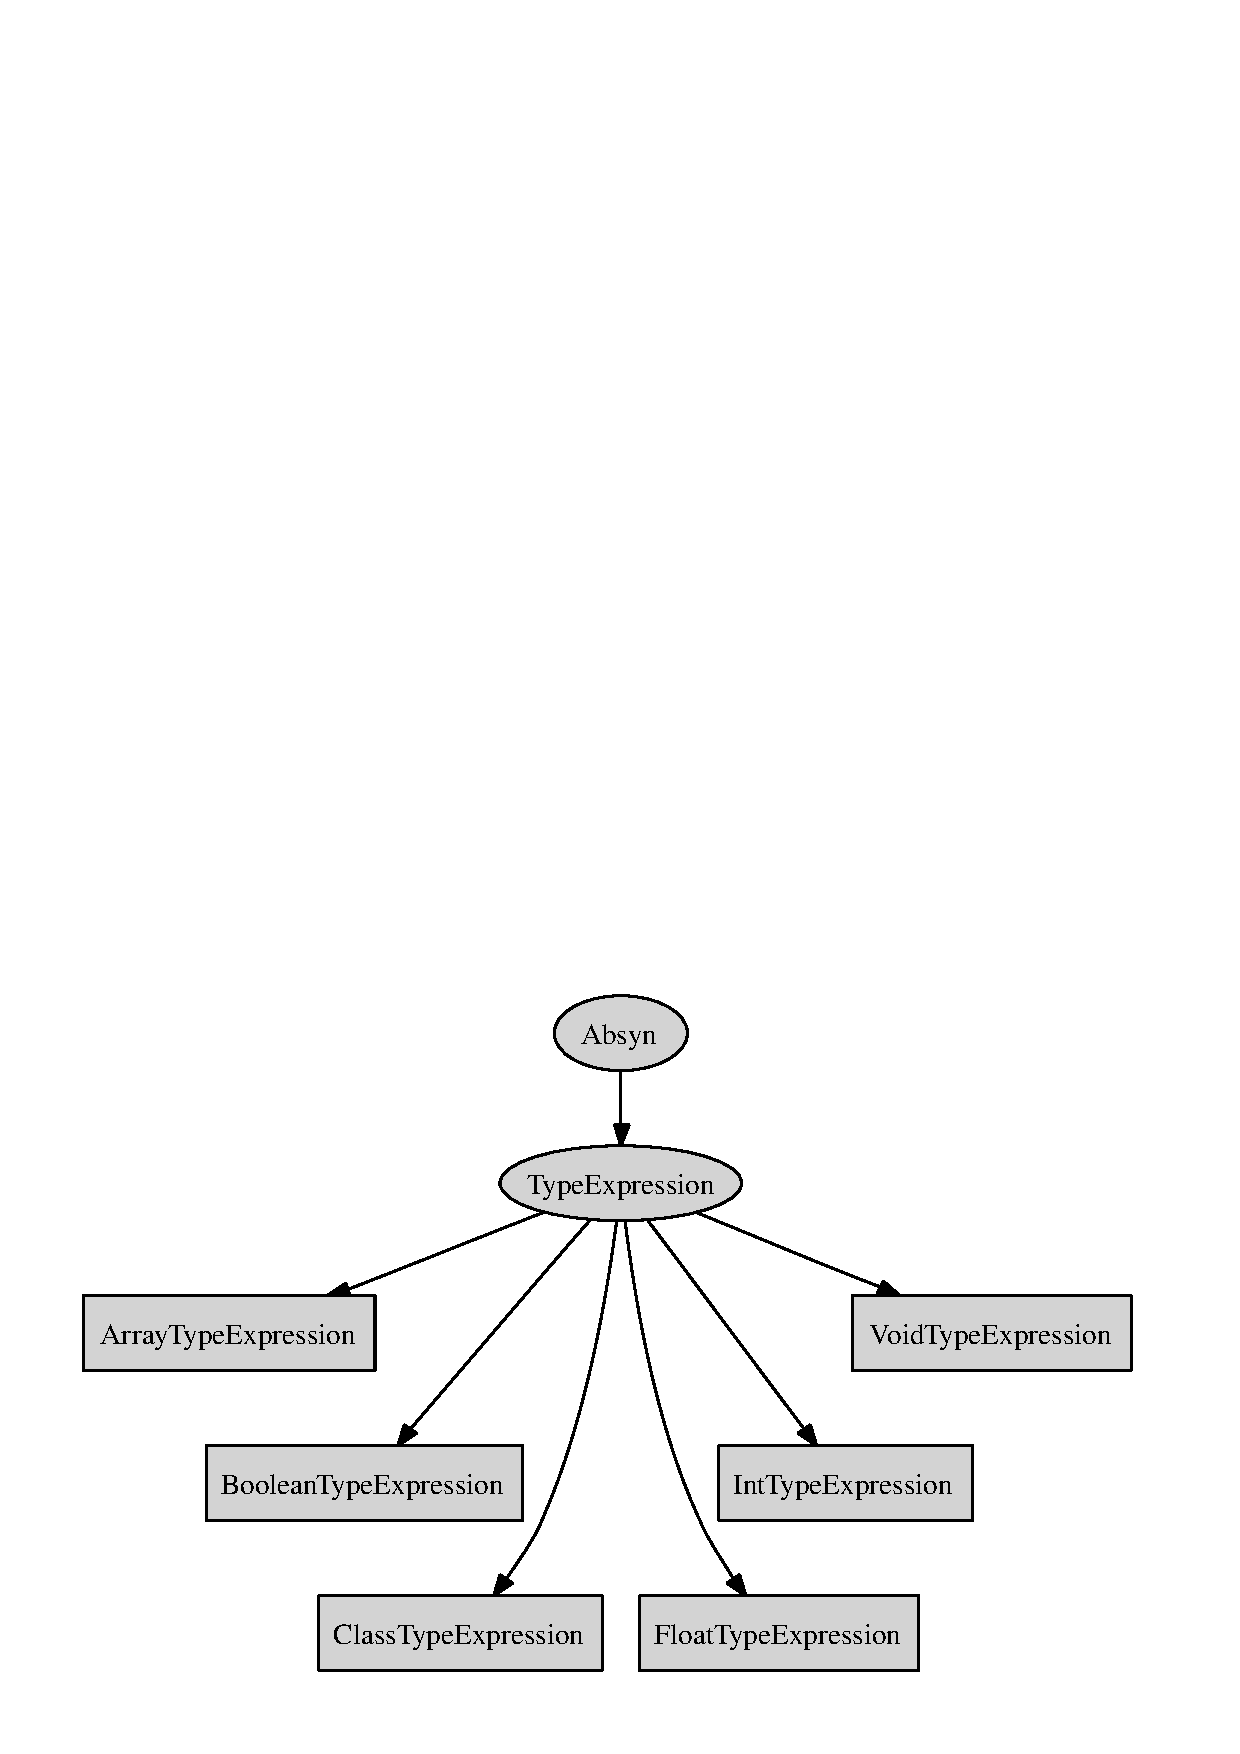
\epsfig{file = types_hierarchy.pdf, width = 14cm}
\end{center}
\caption{La struttura gerarchica delle classi di sintassi astratta per
         i tipi. Le classi astratte sono indicate con un
         ovale, quelle concrete con un rettangolo.}
  \label{fig:types_hierarchy}
\end{figure}

\begin{figure}[t]
\begin{verbatim}
  public class Symbol implements Comparable {
    // alcuni simboli usati di frequente
    public static final Symbol THIS = mk("this");
    public static final Symbol OBJECT = mk("Object");
    public static final Symbol STRING = mk("String");
    private String name;   // il nome del simbolo

    private Symbol(String name) { // si noti: e' private!
      this.name = name;
    }

    // possiamo creare simboli solo con questo metodo
    public static Symbol mk(String name) {
      // usa una tabella statica per determinare se il simbolo e' gia'
      // stato creato e in tal caso lo ritorna. Altrimenti lo crea,
      // lo aggiunge alla tabella e lo ritorna
    }

    public String toString() { return name; }

    public int compareTo(Object other) {
      if (!(other instanceof Symbol)) return 0;
      return name.compareTo(((Symbol)other).name);
    }
  }
\end{verbatim}
\caption{La classe \texttt{symbol/Symbol.java} che rappresenta gli identificatori Kitten.}
  \label{fig:symbol.Symbol}
\end{figure}

La Figura~\ref{fig:types_hierarchy} mostra la gerarchia delle classi di
sintassi astratta per le espressioni di tipo dei programmi Kitten.
Indichiamo con un ovale una classe astratta (nel senso di Java) e con
un rettangolo una classe concreta. Queste classi vengono istanziate
dalle produzioni che definiscono i tipi Kitten
(si confronti con la Sezione~\ref{subsec:types_specification}):
%
\begin{verbatim}
  type ::=
     ID:id
     {: RESULT = new ClassTypeExpression(idleft,Symbol.mk(id)); :}
   | BOOLEAN:b
     {: RESULT = new BooleanTypeExpression(bleft); :}
   | INT:i
     {: RESULT = new IntTypeExpression(ileft); :}
   | FLOAT:f
     {: RESULT = new FloatTypeExpression(fleft); :}
   | ARRAY:a OF type:t
     {: RESULT = new ArrayTypeExpression(aleft,t); :} ;

  typeplus ::=
     type:t
     {: RESULT = t; :}
   | VOID:v
     {: RESULT = new VoidTypeExpression(vleft); :} ;
\end{verbatim}
%
Il metodo statico \texttt{Symbol.mk()} trasforma il valore lessicale
\texttt{id} di un identificatore \texttt{ID} (\cioe il suo
nome, visto come stringa) in un oggetto della classe
\texttt{symbol/Symbol.java} mostrata in
Figura~\ref{fig:symbol.Symbol}. Tale classe \`e molto simile a
\texttt{java.lang.String}, con l'unica differenza che non
possono esistere due \texttt{symbol.Symbol} che rappresentano lo
stesso identificatore. Questo \`e ottenuto costringendo il programmatore
a creare oggetti tramite un metodo statico \texttt{mk} che tiene traccia
degli identificatori gi\`a creati ed evita di creare doppioni.
Avevamo gi\`a osservato infatti che l'albero di sintassi astratta
usa gli stessi nodi per diverse occorrenze dello stesso identificatore
(Figura~\ref{fig:led_albero}).
Il vantaggio di non avere due oggetti diversi per lo stesso identificatore
sar\`a evidente in fase di analisi semantica, quando dovremo associare
l'uso di un identificare con la sua dichiarazione. Avere lo stesso oggetto
in entrambi i punti di programma semplificher\`a il nostro lavoro
(Capitoli~\ref{chap:recursive_descent} e~\ref{chap:semantical}).

Avendo aggiunto delle azioni semantiche alla grammatica della
Sezione~\ref{sec:java_cup}, dobbiamo anche definire il tipo del valore
semantico dei terminali e dei non terminali della grammatica.
A tal fine modifichiamo come segue le
enumerazioni della Sezione~\ref{subsec:terminals}:
%
\begin{verbatim}
  terminal String ID, STRING;
  terminal Integer INTEGER;
  terminal Float FLOATING;

  non terminal TypeExpression type;
  non terminal TypeExpression typeplus;
\end{verbatim}
%
Le prime tre dichiarazioni dicono che il valore semantico dei token
\texttt{ID}, \texttt{STRING}, \texttt{INTEGER} e \texttt{FLOATING}
\`e lo stesso sintetizzato dall'analizzatore lessicale per Kitten
come valore lessicale per tali token (Capitolo~\ref{chap:lexical}).
Le ultime due dichiarazioni indicano che
il tipo del valore semantico delle espressioni di tipo \`e
la superclasse \texttt{TypeExpression} di tutte le classi astratte per
le espressioni di tipo (Figura~\ref{fig:types_hierarchy}).
%
\subsection{Le classi di sintassi astratta per le espressioni e per
            i leftvalue}
  \label{subsec:expressions_abstract}
%
La Figura~\ref{fig:expressions_hierarchy} mostra la gerarchia delle classi
di sintassi astratta per espressioni e leftvalue.
Vogliamo che il non terminale \texttt{exp} per le espressioni abbia
un valore lessicale che sia sottoclasse di \texttt{Expression}. Per
cui dichiariamo:
%
\begin{verbatim}
  non terminal Expression exp;
\end{verbatim}

Per \emph{letterale} si intende una rappresentazione sintattica di un
valore. Le classi astratte per i letterali sono create con le produzioni:
%
\begin{verbatim}
  exp ::=
     INTEGER:i
     {: RESULT = new IntLiteral(ileft,i.intValue()); :}
   | FLOATING:f
     {: RESULT = new FloatLiteral(fleft,f.floatValue()) ; :}
   | STRING:s
     {: RESULT = new StringLiteral(sleft,s); :}
\end{verbatim}
%
Ricordiamo che questi sono i soli tre token che abbiano un valore
lessicale associato, oltre ad \texttt{ID}.

Le classi di sintassi astratta per i leftvalue sono sottoclassi di
\texttt{Expression}, il che \`e sensato essendo i leftvalue dei casi
particolari di espressioni. Tali classi di sintassi astratta
sono create dalle produzioni:
%
\begin{figure}[t]
\begin{center}
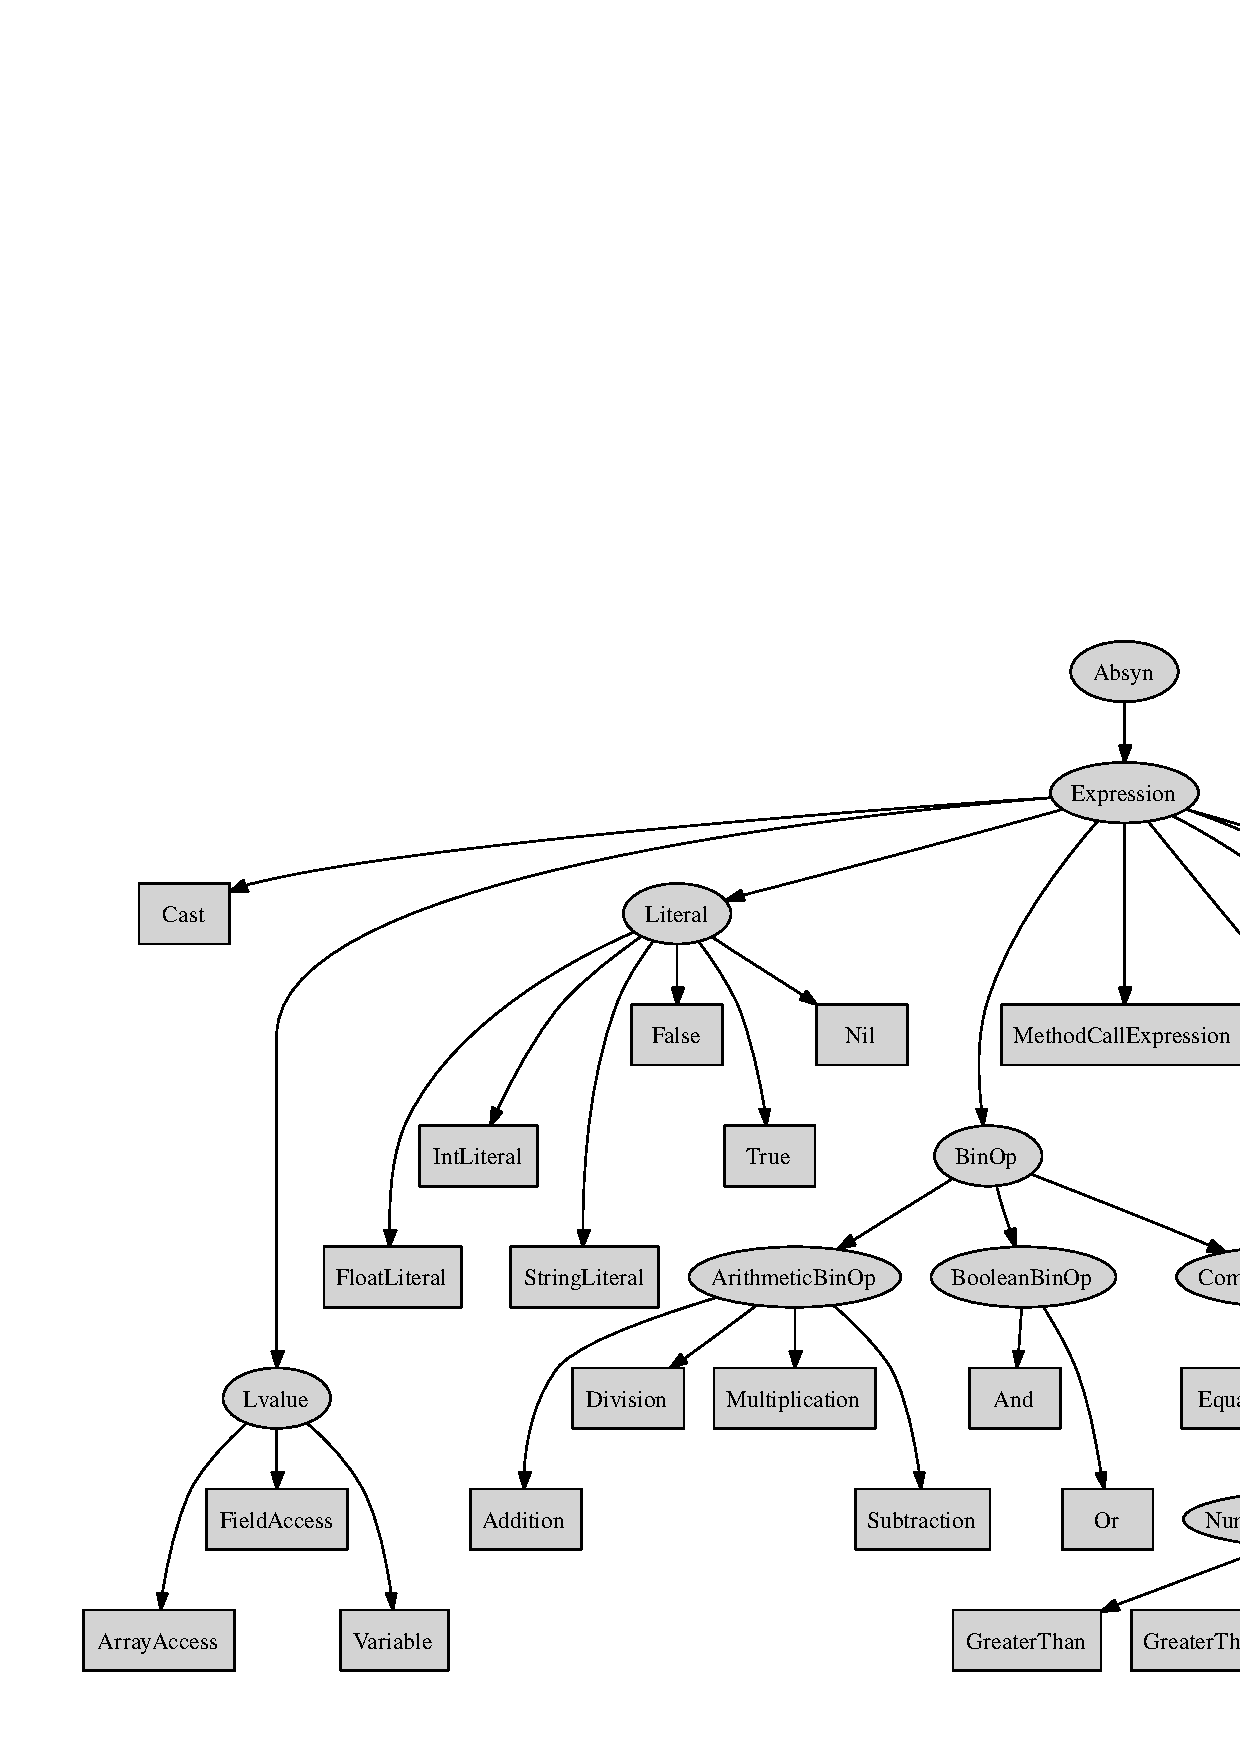
\epsfig{file = expressions_hierarchy.pdf, width = 15.5cm}
\end{center}
\caption{La struttura gerarchica delle classi di sintassi astratta per
         espressioni e leftvalue. Le classi astratte sono indicate con un
         ovale, quelle concrete con un rettangolo.}
  \label{fig:expressions_hierarchy}
\end{figure}
%
\begin{verbatim}
  lvalue ::=
     ID:id
     {: RESULT = new Variable(idleft,Symbol.mk(id)); :}
   | exp:receiver DOT:d ID:field
     {: RESULT = new FieldAccess(dleft,receiver,Symbol.mk(field)); :}
   | exp:array LBRACK:b exp:index RBRACK
     {: RESULT = new ArrayAccess(bleft,array,index); :} ;
\end{verbatim}

La Figura~\ref{fig:expressions_hierarchy} mostra la complessit\`a della
gerarchia delle classi di sintassi astratta per le
espressioni che sono operatori binari. Tali espressioni
sono in primo luogo divise
in \emph{aritmetiche} (\texttt{ArithmeticBinOp}),
\emph{booleane} (\texttt{BooleanBinOp}) e
\emph{di confronto} (\texttt{ComparisonBinOp}).
Queste ultime sono a loro volta divise in operazioni di confronto
che possono operare su qualsiasi tipo di valore, come
l'uguaglianza e la disuguaglianza, e in operazioni di confronto
che operano solo su numeri (interi o in virgola mobile),
incluse nella classe \texttt{NumericalComparisonBinOp}.
%
\subsection{Le classi di sintassi astratta per i comandi}
  \label{subsec:commands_abstract}
%
\begin{figure}[t]
\begin{center}
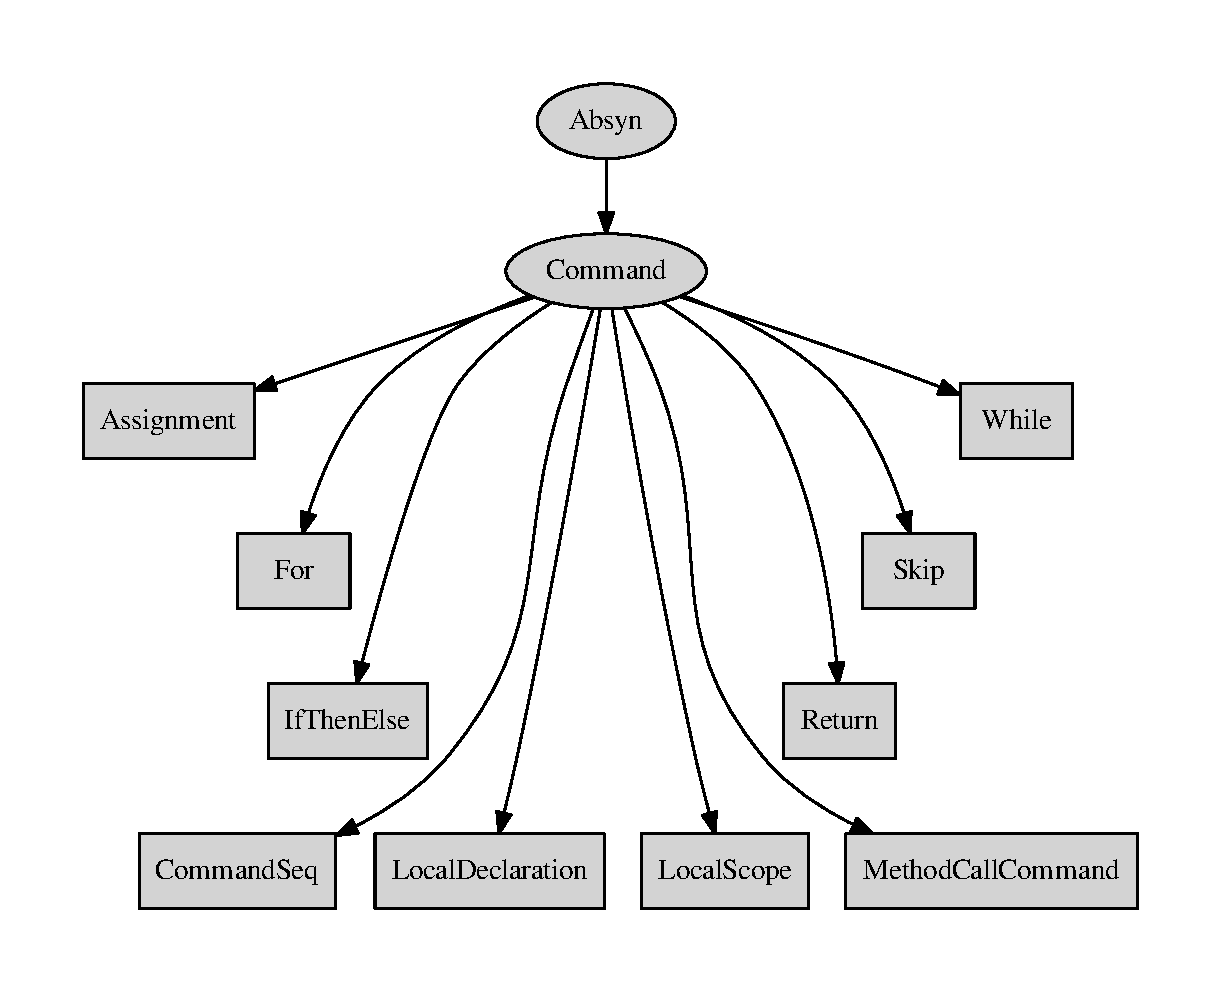
\epsfig{file = commands_hierarchy.pdf, width = 10cm}
\end{center}
\caption{La struttura gerarchica delle classi di sintassi astratta per
         i comandi. Le classi astratte sono indicate con un
         ovale, quelle concrete con un rettangolo.}
  \label{fig:commands_hierarchy}
\end{figure}
%
La Figura~\ref{fig:commands_hierarchy} mostra le classi di sintassi astratta
per i comandi. Si tratta di una gerarchia relativamente semplice.
La classe \texttt{LocalDeclaration} \`e
utilizzata per rappresentare la dichiarazione di una variabile.
La classe \texttt{Skip} \`e usata per rappresentare un comando vuoto,
come per esempio il corpo \verb!{}! del costruttore della classe in
Figura~\ref{fig:fibonacci}.
La classe \texttt{IfThenElse} \`e utilizzata per rappresentare sia il
condizionale semplice che quello composto, \cioe munito del ramo \texttt{else}.
Questo \`e evidente osservando le azioni semantiche per tale comando:
%
\begin{verbatim}
  command ::=
     IF:i LPAREN exp:condition RPAREN THEN command:then
      {: RESULT = new IfThenElse(ileft,condition,then); :}
   | IF:i LPAREN exp:condition RPAREN THEN command:then ELSE command:else
      {: RESULT = new IfThenElse(ileft,condition,then,else); :}
\end{verbatim}
%
Il costruttore a soli tre argomenti della classe
\texttt{absyn/IfThenElse.java} \`e definito in modo da chiamare
quello a quattro argomenti passando come quarto argomento un ramo
\texttt{else} vuoto, \cioe un'oggetto creato come
\texttt{new Skip(pos)}. In questo modo d'ora in poi possiamo sempre
assumere che i condizionali abbiano sempre un ramo \texttt{else}.

Le classi astratte per i comandi hanno un campo
\texttt{next} che lega in sequenza comandi contigui.
Il costruttore di \texttt{absyn/Command.java} annulla tale campo,
che deve essere settato in seguito quando si riconoscono due comandi
contigui. Questo \`e effettuato tramite il metodo \texttt{link()} della
classe \texttt{absyn/Command.java}, utilizzato nelle produzioni per gli
statements:
%
\begin{verbatim}
  statements ::=
     command:cmd
     {: RESULT = cmd; :}
   | command:cmd SEMICOLON statements:next
     {: cmd.link(next); RESULT = cmd; :} ;
\end{verbatim}

Anche per i comandi e gli statement
dobbiamo dichiarare il tipo del loro valore semantico, che \`e la
superclasse di tutte le classi di sintassi astratta per i comandi:
%
\begin{verbatim}
  non terminal Command statements;
  non terminal Command command;
\end{verbatim}
%
\subsection{Le classi di sintassi astratta per le classi Kitten}
  \label{subsec:classes_abstract}
%
\begin{figure}[t]
\begin{center}
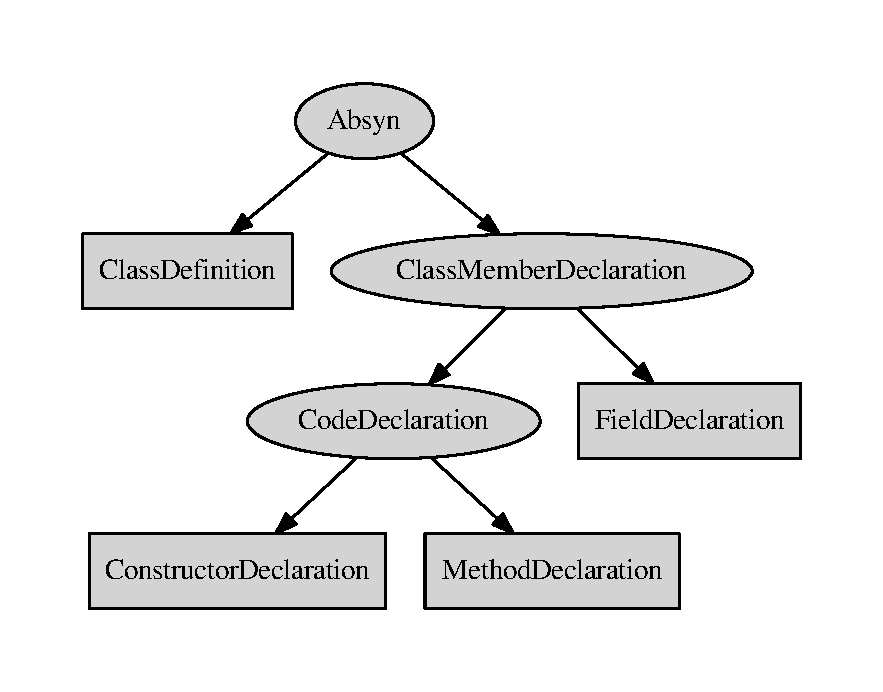
\epsfig{file = classes_hierarchy.pdf, width = 11cm}
\end{center}
\caption{La struttura gerarchica delle classi di sintassi astratta usate
         per rappresentare le classi Kitten.
         Le classi astratte sono indicate con un
         ovale, quelle concrete con un rettangolo.}
  \label{fig:classes_hierarchy}
\end{figure}
%
La Figura~\ref{fig:classes_hierarchy} mostra le classi di sintassi astratta
utilizzate per rappresentare la sintassi delle classi
Kitten. Una classe Kitten \`e rappresentata da un oggetto
di classe \texttt{ClassDefinition} al cui interno si trova una
lista di \texttt{ClassMemberDeclaration}. Ciascuna di tali dichiarazioni
dichiara un membro della classe, che pu\`o essere la dichiarazione di
un campo, di un costruttore o di un metodo.

Le produzioni che istanziano queste classi di sintassi astratta sono le
seguenti (si confronti con la Sezione~\ref{subsec:classes_specification}):
%
\begin{verbatim}
  class ::=
     CLASS:c ID:name LBRACE class_members:declarations RBRACE
      {: RESULT = new ClassDefinition
        (cleft,Symbol.mk(name),Symbol.OBJECT,declarations); :}
   | CLASS:c ID:name EXTENDS ID:superclass
       LBRACE class_members:declarations RBRACE
      {: RESULT = new ClassDefinition
        (cleft,Symbol.mk(name),Symbol.mk(superclass),declarations); :} ;

  class_members ::=
      {: RESULT = null; :}
   | FIELD:f type:t ID:name class_members:next
      {: RESULT = new FieldDeclaration(fleft,t,sym(name),next); :}
   | CONSTRUCTOR:c LPAREN formals:formals RPAREN command:body
       class_members:next
      {: RESULT = new ConstructorDeclaration(cleft,formals,body,next); :}
   | METHOD:m typeplus:returnType ID:name LPAREN formals:formals RPAREN
       command:body class_members:next
      {: RESULT = new MethodDeclaration
        (mleft,returnType,sym(name),formals,body,next); :} ;
\end{verbatim}
%
Si noti che nel caso in cui la superclasse di una classe Kitten non \`e
specificata si assume che essa sia \texttt{Object}, in modo che possiamo
sempre assumere che una classe Kitten abbia specificata la sua superclasse.

I tipi dei non terminali sono dichiarati come:
%
\begin{verbatim}
  non terminal ClassDefinition         class;
  non terminal ClassMemberDeclaration  class_members;
\end{verbatim}
%
\begin{figure}
\begin{center}
{\scriptsize
\begin{tabular}{l}
\textit{Absyn()} \\
\texttt{Addition(Expression left, Expression right)} \\
\texttt{And(Expression left, Expression right)} \\
\textit{ArithmeticBinOp(Expression left, Expression right)} \\
\texttt{ArrayAccess(Expression array, Expression index)} \\
\texttt{ArrayTypeExpression(TypeExpression elementsType)} \\
\texttt{Assignment(Lvalue lvalue, Expression rvalue)} \\
\textit{BinOp(Expression left, Expression right)} \\
\textit{BooleanBinOp(Expression left, Expression right)} \\
\texttt{BooleanTypeExpression()} \\
\texttt{Cast(TypeExpression type, Expression expression)} \\
\texttt{ClassDefinition(Symbol name, Symbol superclassName, ClassMemberDeclaration declaration)} \\
\textit{ClassMemberDeclaration(ClassMemberDeclaration next)} \\
\texttt{ClassTypeExpression(Symbol name)} \\
\textit{CodeDeclaration(FormalParameters formals, Command body, ClassMemberDeclaration next)} \\
\textit{Command()} \\
\textit{ComparisonBinOp(Expression left, Expression right)} \\
\texttt{ConstructorDeclaration(FormalParameters formals, Command body, ClassMemberDeclaration next)} \\
\texttt{Division(Expression left, Expression right)} \\
\texttt{Equal(Expression left, Expression right)} \\
\textit{Expression()} \\
\texttt{ExpressionSeq(Expression head, ExpressionSeq tail)} \\
\texttt{False()} \\
\texttt{FieldAccess(Expression receiver, Symbol name)} \\
\texttt{FieldDeclaration(TypeExpression type, Symbol name, ClassMemberDeclaration next)} \\
\texttt{FloatLiteral(float value)} \\
\texttt{FloatTypeExpression()} \\
\texttt{For(Command initialisation, Expression condition, Command update, Command body)} \\
\texttt{FormalParameters(TypeExpression type, Symbol name, FormalParameters next)} \\
\texttt{GreaterThan(Expression left, Expression right)} \\
\texttt{GreaterThanOrEqual(Expression left, Expression right)} \\
\texttt{IfThenElse(Expression condition, Command then, Command else)} \\
\texttt{IntLiteral(float value)} \\
\texttt{IntTypeExpression()} \\
\texttt{LessThan(Expression left, Expression right)} \\
\texttt{LessThanOrEqual(Expression left, Expression right)} \\
\textit{Literal()} \\
\texttt{LocalDeclaration(TypeExpression type, Symbol name, Expression initialiser)} \\
\texttt{LocalScope(Command body)} \\
\textit{Lvalue()} \\
\texttt{MethodCallCommand(Expression receiver, Symbol name, ExpressionSeq actuals)} \\
\texttt{MethodCallExpression(Expression receiver, Symbol name, ExpressionSeq actuals)} \\
\texttt{MethodDeclaration(TypeExpression returnType, Symbol name, FormalParameters formals,}\\
\hspace*{21ex}\texttt{Command body, ClassMemberDeclaration next)} \\
\texttt{Minus(Expression expression)} \\
\texttt{Multiplication(Expression left, Expression right)} \\
\texttt{NewArray(TypeExpression elementsType, Expression size)} \\
\texttt{NewObject(Symbol className, ExpressionSeq actuals)} \\
\texttt{Nil()} \\
\texttt{Not(Expression expression)} \\
\texttt{NotEqual(Expression left, Expression right)} \\
\textit{NumericalComparisonBinOp(Expression left, Expression right)} \\
\texttt{Or(Expression left, Expression right)} \\
\texttt{Return(Expression returned)} \\
\texttt{Skip()} \\
\texttt{StringLiteral(String value)} \\
\texttt{Subtraction(Expression left, Expression right)} \\
\texttt{True()} \\
\textit{TypeExpression()} \\
\texttt{Variable(Symbol name)} \\
\texttt{VoidTypeExpression()} \\
\texttt{While(Expression condition, Command body)}
\end{tabular}
}
\end{center}
\caption{Una visione d'insieme delle classi di sintassi astratta del linguaggio Kitten. Le classi in \emph{italico} sono classi astratte, nel senso di Java.}
  \label{fig:abstract_classes}
\end{figure}
%
\subsection{Un riassunto delle classi di sintassi astratta di Kitten}
  \label{subsec:abstract_classes}
%
In Figura~\ref{fig:abstract_classes} riportiamo un elenco riassuntivo delle
classi di sintassi astratta di Kitten. Per ogni classe riportiamo il
costruttore, che d\`a anche informazione sul contenuto degli oggetti di tale
classe. Per esempio, la notazione:
%
\begin{verbatim}
  Addition(Expression left, Expression right)
\end{verbatim}
%
indica che la classe di sintassi astratta \texttt{absyn/Addition.java}
ha due campi, \texttt{left} e \texttt{right}, di tipo
\texttt{Expression}. Il suo costruttore ha in effetti \emph{tre} parametri:
oltre ai due riportati, \`e sottointeso anche un primo parametro \texttt{pos}
di tipo \texttt{int} che indica la posizione del file sorgente in cui segnalare
un errore in fase di analisi semantica se qualcosa non torna su questa parte
di sintassi. Per semplicit\`a, in Figura~\ref{fig:abstract_classes}
non abbiamo riportato tale ulteriore parametro.

La Figura~\ref{fig:abstract_classes} \`e compatibile
con l'albero di sintassi astratta in Figura~\ref{fig:led_albero}.
Per esempio, il nodo etichettato con
\texttt{Not} in Figura~\ref{fig:led_albero}
rappresenta un oggetto di classe \texttt{Not} il cui
costruttore, in Figura~\ref{fig:abstract_classes}, ha intestazione
\texttt{Not(Expression expression)}. L'espressione negata \`e infatti
legata in Figura~\ref{fig:led_albero} tramite un arco etichettato con
\texttt{expression} a un nodo di tipo \texttt{FieldAccess}, che
\`e sottoclasse di \texttt{Expression}
(Figura~\ref{fig:expressions_hierarchy}).
Tale nodo di tipo \texttt{FieldAccess} \`e poi legato, in
Figura~\ref{fig:led_albero}, tramite due archi etichettati con
\texttt{receiver} e \texttt{name}, a due nodi di tipo, rispettivamente,
\texttt{Variable} e \texttt{Symbol} (rettangolare). Questo
rispetta il costruttore di \texttt{FieldAccess} in
Figura~\ref{fig:abstract_classes}, che \`e
\texttt{FieldAccess(Expression receiver, Symbol name)}.
Si noti che \texttt{Variable} \`e una sottoclasse di \texttt{Expression}
(Figura~\ref{fig:expressions_hierarchy}).

Ricordiamo che ulteriori informazioni sulle classi di sintassi astratta sono
disponibili con la distribuzione di Kitten, sotto forma di documentazione
JavaDoc.
